\begin{filecontents*}{\jobname.xmpdata}
\Title{EvalSMSI}
\Author{Michel Dubois}
\Subject{Evaluation du SMSI}
\Publisher{Michel Dubois}
\end{filecontents*}

\documentclass[a4paper,10pt]{article}

\usepackage[a-1b]{pdfx}

\usepackage[T1]{fontenc}
\usepackage[utf8]{inputenc}
\usepackage[french]{babel}
\usepackage{utopia}

\usepackage{titlesec}
\usepackage{xcolor}
\usepackage{hyperref}
\usepackage{graphicx}
\usepackage[protrusion=true,expansion=true]{microtype}
\usepackage{amsmath, amssymb}
\usepackage{fancyhdr, fancyvrb}
\usepackage{geometry}
\usepackage{lastpage}
\usepackage{mathtools, amsthm}
\usepackage{multirow}
\usepackage{textcomp} % pour la commande textcomp \textquotesingle
\usepackage{array, colortbl}
\usepackage{longtable,booktabs}
\usepackage{makecell}
\usepackage{tikz}
\usepackage{pgfplots}
\usetikzlibrary{positioning, backgrounds, fit}
\pgfplotsset{compat=newest}

\definecolor{myGrey}{RGB}{50,50,50}
\definecolor{myBlue}{RGB}{30,111,158}
\definecolor{myWaterGreen}{RGB}{30,158,111}
\definecolor{myBrown}{RGB}{158,111,30}
\definecolor{myPurple}{RGB}{158,30,111}
\definecolor{myViolet}{RGB}{111,30,158}
\definecolor{myRed}{RGB}{158,30,30}
\definecolor{myGreen}{RGB}{30,158,30}
\definecolor{myRose}{RGB}{240,30,128}
\definecolor{myGold}{RGB}{224,186,72}
\definecolor{myOrange}{RGB}{240,125,30}
\definecolor{myBackground}{RGB}{29,30,25}
\definecolor{myLightBackground}{RGB}{213,202,184}
\definecolor{myBeige}{RGB}{233,228,219}
\definecolor{myTitleColor}{RGB}{112,113,115}
\definecolor{mySectionColor}{RGB}{64,110,150}
\definecolor{mySubSectionColor}{RGB}{91,155,213}

\titlelabel{\thetitle.\enspace}
\titleformat*{\section}{\bfseries\Large\color{mySectionColor}}
\titleformat*{\subsection}{\bfseries\large\color{mySubSectionColor}}
\titleformat*{\subsubsection}{\bfseries\color{mySubSectionColor}}

\pdfadjustspacing=1
\widowpenalty = 300
\clubpenalty = 300
\hyphenpenalty = 0
\displaywidowpenalty = 10000

\geometry{left=2cm, right=2cm, top=2cm, bottom=2cm}
\setlength{\parindent}{0pt}
\setlength{\parskip}{6pt plus 2pt minus 1pt}
\setlength{\headheight}{20.0pt}
\renewcommand{\headrulewidth}{0.5pt}
\renewcommand{\footrulewidth}{0.5pt}
\setlength{\columnseprule}{0.5pt}
\setlength{\emergencystretch}{3em}  % prevent overfull lines
\setcounter{tocdepth}{3}
\setcounter{secnumdepth}{5}
\arrayrulecolor{myLightBackground}


\pagestyle{fancy}
\fancyhf{}
\fancyhead[L]{\scriptsize\rightmark}
\fancyfoot[C]{\scriptsize{page~\thepage~sur~\pageref{LastPage}}}

\frenchsetup{StandardItemLabels=false, ItemLabeli=$\bullet$}

\hypersetup{%
	pdfencoding=unicode,
	hypertexnames=false,
	pdfstartview=FitH,
	colorlinks=true,
	urlcolor=myBlue,
	linkcolor=myRed,
	citecolor=myGreen,
	bookmarksnumbered=true,
	bookmarksopen=true,
	bookmarksopenlevel=2,
	pdfborder={0 0 0}
}


\title{Rapport d'évaluation du\\Système de Management de la Sécurité de l'Information\\ \textcolor{myRed}{Etablissement de test2}}

\author{Bruce Banner -- \textcolor{myRed}{Auditeur}}

\date{\today}

\begin{document}

\renewcommand{\labelitemi}{\ensuremath{\bullet}}
\renewcommand{\labelitemii}{\ensuremath{\circ}}
\renewcommand{\labelitemiii}{\ensuremath{\triangleright}}

\maketitle

\bigskip\bigskip\bigskip

\abstract{Ce rapport décrit le résultat de l'évaluation du Système de Management de la Sécurité de l'Information (SMSI) réalisé à \textsl{Etablissement de test2} en 2018. L'évaluation initiale a été contrôlée le \today{} par Bruce Banner. Cette évaluation repose sur un questionnaire établit conformément aux normes ISO~27001 et ISO~27002.}

\bigskip\bigskip\bigskip

\begin{itemize}
\item Directeur de l'établissement: \textsl{ }
\item RSSI de l'établissement: \textsl{Hank Pym}
\end{itemize}

\bigskip\bigskip\bigskip

\begin{center}
\Large{\textcolor{myRed}{Rapport validé}}
\end{center}

\bigskip\bigskip\bigskip

\begin{flushright}
\textcolor{myRed}{Original signé}

\textcolor{myRed}{Bruce Banner}\end{flushright}

\clearpage

\textcolor{myRed}{\tableofcontents}

\clearpage



\begin{center}

{\Large{\textcolor{myRed}{Rapport imprimé par l'établissement le \today.}}}

\end{center}

\clearpage


\section{Analyse de l'évaluation du SMSI pour l'année 2018}

\subsection{Introduction}

\subsubsection{Le modèle PDCA et la roue de Deming}

La roue de Deming est une illustration de la méthode qualité PDCA (Plan-Do-Check-Act). Son nom vient du statisticien William Edwards Deming. Ce dernier n'a pas inventé le principe du PDCA, mais il l'a popularisé dans les années 50 en présentant cet outil au Nippon Keidanren.

La méthode comporte quatre étapes, chacune entraînant l'autre, et vise à établir un cercle vertueux. Sa mise en place doit permettre d'améliorer sans cesse la qualité d'un produit, d'une œuvre, d'un service...

\begin{description}
	\item[Plan] Préparer, Planifier (ce que l'on va réaliser);
	\item[Do] Développer, réaliser, mettre en œuvre;
	\item[Check] Contrôler, vérifier;
	\item[Act] Agir, réagir
\end{description}

\subsubsection{Le modèle PDCA appliqué au SMSI}

Appliqué au Système de Management de la Sécurité de l'Information, le PDCA se traduit selon le schéma suivant:

\begin{figure}[ht]
	\begin{center}
	\begin{tikzpicture}
		\def\dist{80pt}
		\def\s{50pt}
		\tikzstyle{nom} = [color=myBlue, text width=80pt, font=\bfseries, inner sep=0pt, text badly centered]
		\tikzstyle{comment} = [color=myRed, text width=60pt, font=\footnotesize, inner sep=0pt, text badly centered]
		\tikzstyle{myedge} = [-latex, color=myRed, line width=0.5pt, double, double distance=4pt, shorten <=24pt, shorten >=24pt]

		\node (p) {
\includegraphics[width=\s]{pict/plan.png}};
		\node (a) [below left=\dist of p] {
\includegraphics[width=\s]{pict/act.png}};
		\node (d) [below right=\dist of p] {
\includegraphics[width=\s]{pict/do.png}};
		\node (c) [below right=\dist of a] {
\includegraphics[width=\s]{pict/check.png}};

		\node (pimg) [nom, below=-6pt of p] {Planifier (Plan)};
		\node (dimg) [nom, below=-6pt of d] {Déployer (Do)};
		\node (cimg) [nom, below=-6pt of c] {Contrôler (Check)};
		\node (aimg) [nom, below=-6pt of a] {Agir (Act)};

		\node [comment, below=0pt of pimg] {Etablissement de la politique SSI};
		\node [comment, below=0pt of dimg] {Mise en oeuvre des mesures SSI};
		\node [comment, below=0pt of cimg] {Contrôle et audit};
		\node [comment, below=0pt of aimg] {Actions correctives};

		\draw (p) edge[myedge, out=0, in=90] (d);
		\draw (d) edge[myedge, out=270, in=0] (c);
		\draw (c) edge[myedge, out=180, in=270] (a);
		\draw (a) edge[myedge, out=90, in=180] (p);
	\end{tikzpicture}
	\end{center}
	\caption{Le PDCA appliqué au SMSI}
\end{figure}

\begin{description}
	\item[Planifier] \'Etablir la politique, les objectifs, les processus et les procédures du SMSI relatives à la gestion du risque et à l'amélioration de la sécurité de l'information de manière à fournir des résultats conformément aux politiques et aux objectifs globaux de l'organisme;
	\item[Déployer] Mettre en \oe{}uvre et exploiter la politique, les mesures, les processus et les procédures du SMSI;
	\item[Contrôler] \'Evaluer et, le cas échéant, mesurer les performances des processus par rapport à la politique, aux objectifs et à l'expérience pratique et rendre compte des résultats à la direction pour réexamen;
	\item[Agir] Entreprendre les actions correctives et préventives, sur la base des résultats de l'audit interne du SMSI et la revue de direction, ou d'autres informations pertinentes, pour une amélioration continue dudit système.
\end{description}

\subsection{Explications préliminaires}

\subsubsection{Mode de calcul des notes}

Chacune des questions possède une pondération permettant de les hiérarchiser. La note de chaque thème est calculée en réalisant une moyenne pondérée de ses questions. Les thèmes sont indépendants entre eux et possèdent tous une note représentative des problématiques qu'ils abordent.

Formule de calcul de la note de chaque thème:

$$ N=\frac{\sum_{i=1}^{n}{\left( P_Q \times E_Q \right)}}{\sum_{i=1}^{n}{P_{Q_i}}} $$

Avec, \textbf{$N$} désignant la note finale du thème, \textbf{$P_Q$} la pondération de la question \textbf{$Q$}, \textbf{$E_Q$} la valeur de l'évaluation pour la question \textbf{$Q$}.

\subsubsection{Détails des cotations}

Pour chaque question, une cotation est définie. Il existe sept choix possible de cotation:

\begin{description}
	\item[Non Applicable] La règle est non applicable ou à fait l'objet d'une dérogation (à préciser dans le commentaire);
	\item[Inexistant et investissement important] La disposition proposée n'est pas appliquée actuellement et ne le sera pas avant un délai important (mesure non planifiée, mesure nécessitant une étude préalable importante, mesure nécessitant un budget important, etc.);
	\item[Inexistant et investissement peu important] La disposition proposée n'est pas appliquée actuellement, mais le sera rapidement, car sa mise en oeuvre est facile et/ou rapide;
	\item[En cours et demande un ajustement] La disposition proposée est en cours de réalisation (état d'avancement à 30\% au minimum), mais des difficultés sont rencontrées et les plans prévus de réalisation doivent être modifiés;
	\item[En cours] La disposition proposée est en cours de réalisation (état d'avancement à 60\% au minimum) et se déroule sans encombre;
	\item[Existant et demande un ajustement] La disposition est mise en place et il reste quelques ajustements à réaliser pour la rendre totalement opérationnelle (état d'avancement à 90\% au minimum);
	\item[Opérationnel] La disposition est opérationnelle et remplit entièrement les besoins demandés.
 \end{description}


\subsection{Notes obtenues par l'établissement}

\begin{center}
\begin{tabular}{ | >{\centering}m{0.20\textwidth} | >{\raggedright}m{0.30\textwidth} @{$\quad\rightarrow\quad$} >{\raggedright}m{0.10\textwidth} | >{\centering}m{0.15\textwidth} | }
\hline
\multicolumn{4}{| c |}{Notes finales de l'établissement}\tabularnewline
\hline
\'Etablissement & \multicolumn{2}{ c |}{\centering{Détail des notes}} & Note finale \tabularnewline
\hline
\multirow{12}{*}{Etablissement de test2} & \multicolumn{2}{ c |}{} & \tabularnewline
& Sensibilisation & \textcolor{myRed}{$7,00 / 20$} & \tabularnewline
& Connaître le SI & $16,11 / 20$ & \tabularnewline
& Authentifier & \textcolor{myRed}{$7,09 / 20$} & \tabularnewline
& Sécuriser les postes & $16,23 / 20$ & \tabularnewline
& Sécuriser le réseau & $15,03 / 20$ & \tabularnewline
& Sécuriser l'administration & $19,43 / 20$ & \tabularnewline
& Nomadisme & \textcolor{myRed}{$6,74 / 20$} & \tabularnewline
& Update du SI & \textcolor{myRed}{$9,40 / 20$} & \tabularnewline
& Superviser & $14,83 / 20$ & \tabularnewline
& Risques & $20,00 / 20$ & \tabularnewline
 & \multicolumn{2}{ c |}{} & \multirow{-12}{*}{$13,19 / 20$} \tabularnewline
\hline
\end{tabular}
\end{center}

\subsection{Graphes de synthèses de l'établissement}

\begin{figure}[ht]
\begin{center}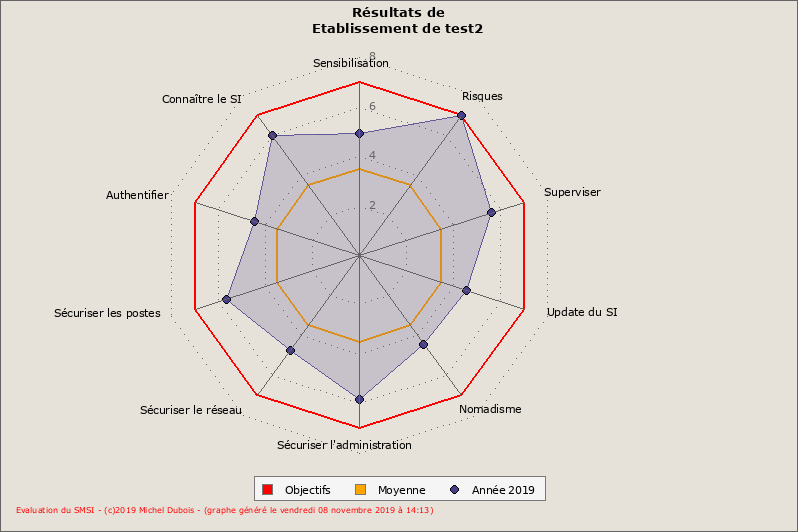
\includegraphics[width=0.90\textwidth]{/home/www/site/evalsmsi/pict/generated/result_par.png}\end{center}
\caption{Résultats par thèmes}
\end{figure}

\begin{figure}[ht]
\begin{center}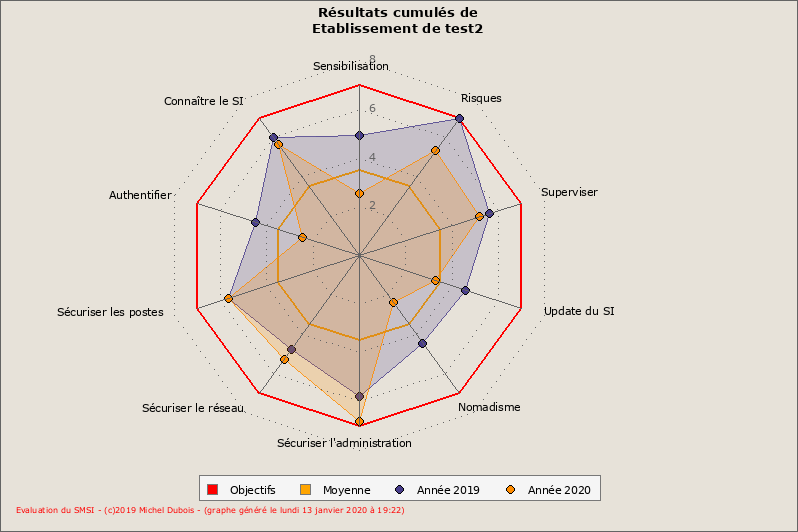
\includegraphics[width=0.90\textwidth]{/home/www/site/evalsmsi/pict/generated/result_par_cumul.png}\end{center}
\caption{Résultats cumulés par thèmes}
\end{figure}

\subsection{Commentaires et conclusion}

\subsubsection{Commentaires de l'établissement}

\par
RAS
\par\subsubsection{Conclusion des évaluateurs}

\par

\par\clearpage


\section{Résultats de l'évaluation du SMSI pour l'année 2018}

\subsection{Sensibiliser et former}

\subsubsection{Former les équipes opérationnelles à la cybersécurité}

\textbf{Question n\textdegree 1.1.1} Un plan de formation à la cybersécurité au profit des équipes opérationnelles  existe et est budgétisé.

\begin{center}
\begin{tabular}{ | >{\centering}m{0.05\textwidth} >{\centering}m{0.25\textwidth} | m{0.50\textwidth} | }
\hline
\multicolumn{2}{|c|}{\textbf{\'Evaluation de l'établissement}} & \centering\textbf{Commentaire} \tabularnewline
\tikz{\node [rectangle, fill=red, inner sep=10pt] {};} & \textcolor{myRed}{Inexistant et investissement important (2/7)} & Néant\tabularnewline
\hline
\multicolumn{3}{|>{\centering}p{0.80\textwidth}|}{\textbf{Commentaire évaluateurs}}\tabularnewline
\multicolumn{3}{|>{\raggedright}p{0.80\textwidth}|}{\textcolor{myBlue}{Avis conforme}}\tabularnewline
\hline
\multicolumn{3}{|c|}{\textbf{Recommandations}}\tabularnewline
\multicolumn{3}{|>{\raggedright}p{0.80\textwidth}|}{Le plan de formation est intégré au dossier de cybersécurité de l'entité.}\tabularnewline
\hline
\end{tabular}
\end{center}
\bigskip

\textbf{Question n\textdegree 1.1.2} Le plan de formation des équipes opérationnelles est spécifique à chaque métier (administrateur, chef de projet, développeur,...)

\begin{center}
\begin{tabular}{ | >{\centering}m{0.05\textwidth} >{\centering}m{0.25\textwidth} | m{0.50\textwidth} | }
\hline
\multicolumn{2}{|c|}{\textbf{\'Evaluation de l'établissement}} & \centering\textbf{Commentaire} \tabularnewline
\tikz{\node [rectangle, fill=red, inner sep=10pt] {};} & \textcolor{myRed}{Inexistant et investissement faible (3/7)} & Néant\tabularnewline
\hline
\multicolumn{3}{|>{\centering}p{0.80\textwidth}|}{\textbf{Commentaire évaluateurs}}\tabularnewline
\multicolumn{3}{|>{\raggedright}p{0.80\textwidth}|}{\textcolor{myBlue}{Avis conforme}}\tabularnewline
\hline
\multicolumn{3}{|c|}{\textbf{Recommandations}}\tabularnewline
\multicolumn{3}{|>{\raggedright}p{0.80\textwidth}|}{Chaque métier nécessite une approche spécifique de la cybersécurité. Par exemple, le développeur pourra être sensibilisé à la gestion sécurisé de la mémoire, tandis que l'administrateur apprendra les principes de la configuration sécurisée d'un système d'exploitation et que le chef de projet assimilera l'intégration de la cybersécurité dans la gestion de projet.}\tabularnewline
\hline
\end{tabular}
\end{center}
\bigskip

\textbf{Question n\textdegree 1.1.3} La formation à la cybersécurité des équipes opérationnelles couvre le volet juridique.

\begin{center}
\begin{tabular}{ | >{\centering}m{0.05\textwidth} >{\centering}m{0.25\textwidth} | m{0.50\textwidth} | }
\hline
\multicolumn{2}{|c|}{\textbf{\'Evaluation de l'établissement}} & \centering\textbf{Commentaire} \tabularnewline
\tikz{\node [rectangle, fill=red, inner sep=10pt] {};} & \textcolor{myRed}{Inexistant et investissement important (2/7)} & Néant\tabularnewline
\hline
\multicolumn{3}{|>{\centering}p{0.80\textwidth}|}{\textbf{Commentaire évaluateurs}}\tabularnewline
\multicolumn{3}{|>{\raggedright}p{0.80\textwidth}|}{\textcolor{myBlue}{Avis conforme}}\tabularnewline
\hline
\multicolumn{3}{|c|}{\textbf{Recommandations}}\tabularnewline
\multicolumn{3}{|>{\raggedright}p{0.80\textwidth}|}{Néant}\tabularnewline
\hline
\end{tabular}
\end{center}
\bigskip

\textbf{Question n\textdegree 1.1.4} La formation à la cybersécurité des équipes opérationnelles détaille les principaux risques et menaces.

\begin{center}
\begin{tabular}{ | >{\centering}m{0.05\textwidth} >{\centering}m{0.25\textwidth} | m{0.50\textwidth} | }
\hline
\multicolumn{2}{|c|}{\textbf{\'Evaluation de l'établissement}} & \centering\textbf{Commentaire} \tabularnewline
\tikz{\node [rectangle, fill=red, inner sep=10pt] {};} & \textcolor{myRed}{Inexistant et investissement important (2/7)} & Néant\tabularnewline
\hline
\multicolumn{3}{|>{\centering}p{0.80\textwidth}|}{\textbf{Commentaire évaluateurs}}\tabularnewline
\multicolumn{3}{|>{\raggedright}p{0.80\textwidth}|}{\textcolor{myBlue}{Avis conforme}}\tabularnewline
\hline
\multicolumn{3}{|c|}{\textbf{Recommandations}}\tabularnewline
\multicolumn{3}{|>{\raggedright}p{0.80\textwidth}|}{Néant}\tabularnewline
\hline
\end{tabular}
\end{center}
\bigskip

\textbf{Question n\textdegree 1.1.5} La formation à la cybersécurité des équipes opérationnelles couvre les notions de maintien en condition de sécurité.

\begin{center}
\begin{tabular}{ | >{\centering}m{0.05\textwidth} >{\centering}m{0.25\textwidth} | m{0.50\textwidth} | }
\hline
\multicolumn{2}{|c|}{\textbf{\'Evaluation de l'établissement}} & \centering\textbf{Commentaire} \tabularnewline
\tikz{\node [rectangle, fill=red, inner sep=10pt] {};} & \textcolor{myRed}{Inexistant et investissement important (2/7)} & Néant\tabularnewline
\hline
\multicolumn{3}{|>{\centering}p{0.80\textwidth}|}{\textbf{Commentaire évaluateurs}}\tabularnewline
\multicolumn{3}{|>{\raggedright}p{0.80\textwidth}|}{\textcolor{myBlue}{Avis conforme}}\tabularnewline
\hline
\multicolumn{3}{|c|}{\textbf{Recommandations}}\tabularnewline
\multicolumn{3}{|>{\raggedright}p{0.80\textwidth}|}{Néant}\tabularnewline
\hline
\end{tabular}
\end{center}
\bigskip

\textbf{Question n\textdegree 1.1.6} La formation à la cybersécurité des équipes opérationnelles détaille les principes et règles de l'authentification et du contrôle d'accès.

\begin{center}
\begin{tabular}{ | >{\centering}m{0.05\textwidth} >{\centering}m{0.25\textwidth} | m{0.50\textwidth} | }
\hline
\multicolumn{2}{|c|}{\textbf{\'Evaluation de l'établissement}} & \centering\textbf{Commentaire} \tabularnewline
\tikz{\node [rectangle, fill=red, inner sep=10pt] {};} & \textcolor{myRed}{Inexistant et investissement important (2/7)} & Néant\tabularnewline
\hline
\multicolumn{3}{|>{\centering}p{0.80\textwidth}|}{\textbf{Commentaire évaluateurs}}\tabularnewline
\multicolumn{3}{|>{\raggedright}p{0.80\textwidth}|}{\textcolor{myBlue}{Avis conforme}}\tabularnewline
\hline
\multicolumn{3}{|c|}{\textbf{Recommandations}}\tabularnewline
\multicolumn{3}{|>{\raggedright}p{0.80\textwidth}|}{Néant}\tabularnewline
\hline
\end{tabular}
\end{center}
\bigskip

\textbf{Question n\textdegree 1.1.7} La formation à la cybersécurité des équipes opérationnelle traite du paramétrage et du durcissement des systèmes d'information.

\begin{center}
\begin{tabular}{ | >{\centering}m{0.05\textwidth} >{\centering}m{0.25\textwidth} | m{0.50\textwidth} | }
\hline
\multicolumn{2}{|c|}{\textbf{\'Evaluation de l'établissement}} & \centering\textbf{Commentaire} \tabularnewline
\tikz{\node [rectangle, fill=red, inner sep=10pt] {};} & \textcolor{myRed}{Inexistant et investissement important (2/7)} & Néant\tabularnewline
\hline
\multicolumn{3}{|>{\centering}p{0.80\textwidth}|}{\textbf{Commentaire évaluateurs}}\tabularnewline
\multicolumn{3}{|>{\raggedright}p{0.80\textwidth}|}{\textcolor{myBlue}{Avis conforme}}\tabularnewline
\hline
\multicolumn{3}{|c|}{\textbf{Recommandations}}\tabularnewline
\multicolumn{3}{|>{\raggedright}p{0.80\textwidth}|}{Néant}\tabularnewline
\hline
\end{tabular}
\end{center}
\bigskip

\textbf{Question n\textdegree 1.1.8} La formation à la cybersécurité des équipes opérationnelle traite de l'architecture sécurisé des systèmes et des réseaux.

\begin{center}
\begin{tabular}{ | >{\centering}m{0.05\textwidth} >{\centering}m{0.25\textwidth} | m{0.50\textwidth} | }
\hline
\multicolumn{2}{|c|}{\textbf{\'Evaluation de l'établissement}} & \centering\textbf{Commentaire} \tabularnewline
\tikz{\node [rectangle, fill=red, inner sep=10pt] {};} & \textcolor{myRed}{Inexistant et investissement faible (3/7)} & Néant\tabularnewline
\hline
\multicolumn{3}{|>{\centering}p{0.80\textwidth}|}{\textbf{Commentaire évaluateurs}}\tabularnewline
\multicolumn{3}{|>{\raggedright}p{0.80\textwidth}|}{\textcolor{myBlue}{Avis conforme}}\tabularnewline
\hline
\multicolumn{3}{|c|}{\textbf{Recommandations}}\tabularnewline
\multicolumn{3}{|>{\raggedright}p{0.80\textwidth}|}{Néant}\tabularnewline
\hline
\end{tabular}
\end{center}
\bigskip

\textbf{Question n\textdegree 1.1.9} Les contrats d'externalisation et d'infogérance contiennent une clause garantissant la formation à la cybersécurité du personnel.

\begin{center}
\begin{tabular}{ | >{\centering}m{0.05\textwidth} >{\centering}m{0.25\textwidth} | m{0.50\textwidth} | }
\hline
\multicolumn{2}{|c|}{\textbf{\'Evaluation de l'établissement}} & \centering\textbf{Commentaire} \tabularnewline
\tikz{\node [rectangle, fill=red, inner sep=10pt] {};} & \textcolor{myRed}{Inexistant et investissement faible (3/7)} & Néant\tabularnewline
\hline
\multicolumn{3}{|>{\centering}p{0.80\textwidth}|}{\textbf{Commentaire évaluateurs}}\tabularnewline
\multicolumn{3}{|>{\raggedright}p{0.80\textwidth}|}{\textcolor{myBlue}{Avis conforme}}\tabularnewline
\hline
\multicolumn{3}{|c|}{\textbf{Recommandations}}\tabularnewline
\multicolumn{3}{|>{\raggedright}p{0.80\textwidth}|}{Néant}\tabularnewline
\hline
\end{tabular}
\end{center}
\bigskip

\subsubsection{Sensibiliser les utilisateurs aux bonnes pratiques élémentaires de sécurité informatique}

\textbf{Question n\textdegree 1.2.1} Un plan de sensibilisation à la cybersécurité au profit des utilisateurs existe et est budgétisé.

\begin{center}
\begin{tabular}{ | >{\centering}m{0.05\textwidth} >{\centering}m{0.25\textwidth} | m{0.50\textwidth} | }
\hline
\multicolumn{2}{|c|}{\textbf{\'Evaluation de l'établissement}} & \centering\textbf{Commentaire} \tabularnewline
\tikz{\node [rectangle, fill=red, inner sep=10pt] {};} & \textcolor{myRed}{Inexistant et investissement faible (3/7)} & Néant\tabularnewline
\hline
\multicolumn{3}{|>{\centering}p{0.80\textwidth}|}{\textbf{Commentaire évaluateurs}}\tabularnewline
\multicolumn{3}{|>{\raggedright}p{0.80\textwidth}|}{\textcolor{myBlue}{Avis conforme}}\tabularnewline
\hline
\multicolumn{3}{|c|}{\textbf{Recommandations}}\tabularnewline
\multicolumn{3}{|>{\raggedright}p{0.80\textwidth}|}{Le plan de sensibilisation des utilisateurs est intégré au dossier de cybersécurité de l'entité.}\tabularnewline
\hline
\end{tabular}
\end{center}
\bigskip

\textbf{Question n\textdegree 1.2.2} La sensibilisation à la cybersécurité des utilisateurs est systématique et renouvelée régulièrement.

\begin{center}
\begin{tabular}{ | >{\centering}m{0.05\textwidth} >{\centering}m{0.25\textwidth} | m{0.50\textwidth} | }
\hline
\multicolumn{2}{|c|}{\textbf{\'Evaluation de l'établissement}} & \centering\textbf{Commentaire} \tabularnewline
\tikz{\node [rectangle, fill=red, inner sep=10pt] {};} & \textcolor{myRed}{Inexistant et investissement faible (3/7)} & Néant\tabularnewline
\hline
\multicolumn{3}{|>{\centering}p{0.80\textwidth}|}{\textbf{Commentaire évaluateurs}}\tabularnewline
\multicolumn{3}{|>{\raggedright}p{0.80\textwidth}|}{\textcolor{myBlue}{Avis conforme}}\tabularnewline
\hline
\multicolumn{3}{|c|}{\textbf{Recommandations}}\tabularnewline
\multicolumn{3}{|>{\raggedright}p{0.80\textwidth}|}{Il est recommandé de sensibiliser les utilisateurs lors de leur arrivée dans l'entité et de renouveler cette sensibilisation tous les 3 ans. La liste des agents sensibilisés à la cybersécurité est conservée dans un registre dédié. Ce registre est intégré au dossier de cybersécurité de l'entité.}\tabularnewline
\hline
\end{tabular}
\end{center}
\bigskip

\textbf{Question n\textdegree 1.2.3} La sensibilisation à la cybersécurité des utilisateurs détaille les règles de la politique de sécurité des systèmes d'informations.

\begin{center}
\begin{tabular}{ | >{\centering}m{0.05\textwidth} >{\centering}m{0.25\textwidth} | m{0.50\textwidth} | }
\hline
\multicolumn{2}{|c|}{\textbf{\'Evaluation de l'établissement}} & \centering\textbf{Commentaire} \tabularnewline
\tikz{\node [rectangle, fill=red, inner sep=10pt] {};} & \textcolor{myRed}{Inexistant et investissement faible (3/7)} & Néant\tabularnewline
\hline
\multicolumn{3}{|>{\centering}p{0.80\textwidth}|}{\textbf{Commentaire évaluateurs}}\tabularnewline
\multicolumn{3}{|>{\raggedright}p{0.80\textwidth}|}{\textcolor{myBlue}{Avis conforme}}\tabularnewline
\hline
\multicolumn{3}{|c|}{\textbf{Recommandations}}\tabularnewline
\multicolumn{3}{|>{\raggedright}p{0.80\textwidth}|}{Néant}\tabularnewline
\hline
\end{tabular}
\end{center}
\bigskip

\textbf{Question n\textdegree 1.2.4} L'entité a élaboré une charte des moyens informatiques précisant les règles et consignes que doivent respecter les utilisateurs.

\begin{center}
\begin{tabular}{ | >{\centering}m{0.05\textwidth} >{\centering}m{0.25\textwidth} | m{0.50\textwidth} | }
\hline
\multicolumn{2}{|c|}{\textbf{\'Evaluation de l'établissement}} & \centering\textbf{Commentaire} \tabularnewline
\tikz{\node [rectangle, fill=red, inner sep=10pt] {};} & \textcolor{myRed}{Inexistant et investissement important (2/7)} & Néant\tabularnewline
\hline
\multicolumn{3}{|>{\centering}p{0.80\textwidth}|}{\textbf{Commentaire évaluateurs}}\tabularnewline
\multicolumn{3}{|>{\raggedright}p{0.80\textwidth}|}{\textcolor{myBlue}{Avis conforme}}\tabularnewline
\hline
\multicolumn{3}{|c|}{\textbf{Recommandations}}\tabularnewline
\multicolumn{3}{|>{\raggedright}p{0.80\textwidth}|}{L'entité peut s'inspirer du guide d'élaboration publié par l'ANSSI (https://bit.ly/2sy5N7e).  La charte des moyens informatiques doit être présentée au CHSCT et intégrée au règlement intérieur de l'entité.}\tabularnewline
\hline
\end{tabular}
\end{center}
\bigskip

\textbf{Question n\textdegree 1.2.5} Chaque utilisateur signe la charte des moyens informatiques.

\begin{center}
\begin{tabular}{ | >{\centering}m{0.05\textwidth} >{\centering}m{0.25\textwidth} | m{0.50\textwidth} | }
\hline
\multicolumn{2}{|c|}{\textbf{\'Evaluation de l'établissement}} & \centering\textbf{Commentaire} \tabularnewline
\tikz{\node [rectangle, fill=red, inner sep=10pt] {};} & \textcolor{myRed}{Inexistant et investissement faible (3/7)} & Néant\tabularnewline
\hline
\multicolumn{3}{|>{\centering}p{0.80\textwidth}|}{\textbf{Commentaire évaluateurs}}\tabularnewline
\multicolumn{3}{|>{\raggedright}p{0.80\textwidth}|}{\textcolor{myBlue}{Avis conforme}}\tabularnewline
\hline
\multicolumn{3}{|c|}{\textbf{Recommandations}}\tabularnewline
\multicolumn{3}{|>{\raggedright}p{0.80\textwidth}|}{La signature de la charte des moyens informatiques est conservées dans un registre dédié. Ce registre est intégré au dossier de cybersécurité de l'entité.}\tabularnewline
\hline
\end{tabular}
\end{center}
\bigskip

\subsubsection{Maîtriser les risques de l'infogérance}

\textbf{Question n\textdegree 1.3.1} Une liste d'exigences précises a été contractualisée avec le prestataires.

\begin{center}
\begin{tabular}{ | >{\centering}m{0.05\textwidth} >{\centering}m{0.25\textwidth} | m{0.50\textwidth} | }
\hline
\multicolumn{2}{|c|}{\textbf{\'Evaluation de l'établissement}} & \centering\textbf{Commentaire} \tabularnewline
\tikz{\node [rectangle, fill=red, inner sep=10pt] {};} & \textcolor{myRed}{Inexistant et investissement important (2/7)} & Néant\tabularnewline
\hline
\multicolumn{3}{|>{\centering}p{0.80\textwidth}|}{\textbf{Commentaire évaluateurs}}\tabularnewline
\multicolumn{3}{|>{\raggedright}p{0.80\textwidth}|}{\textcolor{myBlue}{Avis conforme}}\tabularnewline
\hline
\multicolumn{3}{|c|}{\textbf{Recommandations}}\tabularnewline
\multicolumn{3}{|>{\raggedright}p{0.80\textwidth}|}{L'entité peut s'inspirer du guide sur l'externalisation publié par l'ANSSI (https://bit.ly/2V8e4It)}\tabularnewline
\hline
\end{tabular}
\end{center}
\bigskip

\textbf{Question n\textdegree 1.3.2} La liste d'exigences fixe les modalités de réversibilités du contrat.

\begin{center}
\begin{tabular}{ | >{\centering}m{0.05\textwidth} >{\centering}m{0.25\textwidth} | m{0.50\textwidth} | }
\hline
\multicolumn{2}{|c|}{\textbf{\'Evaluation de l'établissement}} & \centering\textbf{Commentaire} \tabularnewline
\tikz{\node [rectangle, fill=red, inner sep=10pt] {};} & \textcolor{myRed}{Inexistant et investissement important (2/7)} & Néant\tabularnewline
\hline
\multicolumn{3}{|>{\centering}p{0.80\textwidth}|}{\textbf{Commentaire évaluateurs}}\tabularnewline
\multicolumn{3}{|>{\raggedright}p{0.80\textwidth}|}{\textcolor{myBlue}{Avis conforme}}\tabularnewline
\hline
\multicolumn{3}{|c|}{\textbf{Recommandations}}\tabularnewline
\multicolumn{3}{|>{\raggedright}p{0.80\textwidth}|}{Néant}\tabularnewline
\hline
\end{tabular}
\end{center}
\bigskip

\textbf{Question n\textdegree 1.3.3} La liste d'exigence détaille les modalités de réalisation d'audits.

\begin{center}
\begin{tabular}{ | >{\centering}m{0.05\textwidth} >{\centering}m{0.25\textwidth} | m{0.50\textwidth} | }
\hline
\multicolumn{2}{|c|}{\textbf{\'Evaluation de l'établissement}} & \centering\textbf{Commentaire} \tabularnewline
\tikz{\node [rectangle, fill=red, inner sep=10pt] {};} & \textcolor{myRed}{Inexistant et investissement faible (3/7)} & Néant\tabularnewline
\hline
\multicolumn{3}{|>{\centering}p{0.80\textwidth}|}{\textbf{Commentaire évaluateurs}}\tabularnewline
\multicolumn{3}{|>{\raggedright}p{0.80\textwidth}|}{\textcolor{myBlue}{Avis conforme}}\tabularnewline
\hline
\multicolumn{3}{|c|}{\textbf{Recommandations}}\tabularnewline
\multicolumn{3}{|>{\raggedright}p{0.80\textwidth}|}{Néant}\tabularnewline
\hline
\end{tabular}
\end{center}
\bigskip

\textbf{Question n\textdegree 1.3.4} La liste d'exigence détaille les modalités de sauvegarde et de restitution des données dans un format ouvert normalisé.

\begin{center}
\begin{tabular}{ | >{\centering}m{0.05\textwidth} >{\centering}m{0.25\textwidth} | m{0.50\textwidth} | }
\hline
\multicolumn{2}{|c|}{\textbf{\'Evaluation de l'établissement}} & \centering\textbf{Commentaire} \tabularnewline
\tikz{\node [rectangle, fill=red, inner sep=10pt] {};} & \textcolor{myRed}{Inexistant et investissement important (2/7)} & Néant\tabularnewline
\hline
\multicolumn{3}{|>{\centering}p{0.80\textwidth}|}{\textbf{Commentaire évaluateurs}}\tabularnewline
\multicolumn{3}{|>{\raggedright}p{0.80\textwidth}|}{\textcolor{myBlue}{Avis conforme}}\tabularnewline
\hline
\multicolumn{3}{|c|}{\textbf{Recommandations}}\tabularnewline
\multicolumn{3}{|>{\raggedright}p{0.80\textwidth}|}{Néant}\tabularnewline
\hline
\end{tabular}
\end{center}
\bigskip

\textbf{Question n\textdegree 1.3.5} La liste d'exigence détaille la mise en œuvre du maintien à niveau de la sécurité dans le temps.

\begin{center}
\begin{tabular}{ | >{\centering}m{0.05\textwidth} >{\centering}m{0.25\textwidth} | m{0.50\textwidth} | }
\hline
\multicolumn{2}{|c|}{\textbf{\'Evaluation de l'établissement}} & \centering\textbf{Commentaire} \tabularnewline
\tikz{\node [rectangle, fill=red, inner sep=10pt] {};} & \textcolor{myRed}{Inexistant et investissement important (2/7)} & Néant\tabularnewline
\hline
\multicolumn{3}{|>{\centering}p{0.80\textwidth}|}{\textbf{Commentaire évaluateurs}}\tabularnewline
\multicolumn{3}{|>{\raggedright}p{0.80\textwidth}|}{\textcolor{myBlue}{Avis conforme}}\tabularnewline
\hline
\multicolumn{3}{|c|}{\textbf{Recommandations}}\tabularnewline
\multicolumn{3}{|>{\raggedright}p{0.80\textwidth}|}{Néant}\tabularnewline
\hline
\end{tabular}
\end{center}
\bigskip

\textbf{Question n\textdegree 1.3.6} Pour chaque contrat d'externalisation, le prestataire a fourni un plan d'assurance sécurité (PAS).

\begin{center}
\begin{tabular}{ | >{\centering}m{0.05\textwidth} >{\centering}m{0.25\textwidth} | m{0.50\textwidth} | }
\hline
\multicolumn{2}{|c|}{\textbf{\'Evaluation de l'établissement}} & \centering\textbf{Commentaire} \tabularnewline
\tikz{\node [rectangle, fill=red, inner sep=10pt] {};} & \textcolor{myRed}{Inexistant et investissement faible (3/7)} & Néant\tabularnewline
\hline
\multicolumn{3}{|>{\centering}p{0.80\textwidth}|}{\textbf{Commentaire évaluateurs}}\tabularnewline
\multicolumn{3}{|>{\raggedright}p{0.80\textwidth}|}{\textcolor{myBlue}{Avis conforme}}\tabularnewline
\hline
\multicolumn{3}{|c|}{\textbf{Recommandations}}\tabularnewline
\multicolumn{3}{|>{\raggedright}p{0.80\textwidth}|}{L'entité peut s'inspirer du guide sur l'externalisation publié par l'ANSSI (https://bit.ly/2V8e4It)}\tabularnewline
\hline
\end{tabular}
\end{center}
\bigskip

\subsection{Connaître le système d'information}

\subsubsection{Identifier les informations et serveurs les plus sensibles et maintenir un schéma du réseau}

\textbf{Question n\textdegree 2.1.1} La liste des données sensibles existe et est à jour.

\begin{center}
\begin{tabular}{ | >{\centering}m{0.05\textwidth} >{\centering}m{0.25\textwidth} | m{0.50\textwidth} | }
\hline
\multicolumn{2}{|c|}{\textbf{\'Evaluation de l'établissement}} & \centering\textbf{Commentaire} \tabularnewline
\tikz{\node [rectangle, fill=orange, inner sep=10pt] {};} & \textcolor{myRed}{En cours (5/7)} & Néant\tabularnewline
\hline
\multicolumn{3}{|>{\centering}p{0.80\textwidth}|}{\textbf{Commentaire évaluateurs}}\tabularnewline
\multicolumn{3}{|>{\raggedright}p{0.80\textwidth}|}{\textcolor{myBlue}{Avis conforme}}\tabularnewline
\hline
\end{tabular}
\end{center}
\bigskip

\textbf{Question n\textdegree 2.1.2} La liste des données sensibles précise sur quels composants elles sont stockées ou traitées.

\begin{center}
\begin{tabular}{ | >{\centering}m{0.05\textwidth} >{\centering}m{0.25\textwidth} | m{0.50\textwidth} | }
\hline
\multicolumn{2}{|c|}{\textbf{\'Evaluation de l'établissement}} & \centering\textbf{Commentaire} \tabularnewline
\tikz{\node [rectangle, fill=green, inner sep=10pt] {};} & \textcolor{myRed}{Existant et demande un ajustement (6/7)} & Néant\tabularnewline
\hline
\multicolumn{3}{|>{\centering}p{0.80\textwidth}|}{\textbf{Commentaire évaluateurs}}\tabularnewline
\multicolumn{3}{|>{\raggedright}p{0.80\textwidth}|}{\textcolor{myBlue}{Avis conforme}}\tabularnewline
\hline
\end{tabular}
\end{center}
\bigskip

\textbf{Question n\textdegree 2.1.3} Les composants traitants ou hébergeant des données sensibles sont considérés comme critiques.

\begin{center}
\begin{tabular}{ | >{\centering}m{0.05\textwidth} >{\centering}m{0.25\textwidth} | m{0.50\textwidth} | }
\hline
\multicolumn{2}{|c|}{\textbf{\'Evaluation de l'établissement}} & \centering\textbf{Commentaire} \tabularnewline
\tikz{\node [rectangle, fill=orange, inner sep=10pt] {};} & \textcolor{myRed}{En cours (5/7)} & Néant\tabularnewline
\hline
\multicolumn{3}{|>{\centering}p{0.80\textwidth}|}{\textbf{Commentaire évaluateurs}}\tabularnewline
\multicolumn{3}{|>{\raggedright}p{0.80\textwidth}|}{\textcolor{myBlue}{Avis conforme}}\tabularnewline
\hline
\end{tabular}
\end{center}
\bigskip

\textbf{Question n\textdegree 2.1.4} Des mesures de sécurité spécifiques sont décrites pour les composants critiques (sauvegarde, mise à jour, contrôle d'accès)

\begin{center}
\begin{tabular}{ | >{\centering}m{0.05\textwidth} >{\centering}m{0.25\textwidth} | m{0.50\textwidth} | }
\hline
\multicolumn{2}{|c|}{\textbf{\'Evaluation de l'établissement}} & \centering\textbf{Commentaire} \tabularnewline
\tikz{\node [rectangle, fill=green, inner sep=10pt] {};} & \textcolor{myRed}{Existant et demande un ajustement (6/7)} & Néant\tabularnewline
\hline
\multicolumn{3}{|>{\centering}p{0.80\textwidth}|}{\textbf{Commentaire évaluateurs}}\tabularnewline
\multicolumn{3}{|>{\raggedright}p{0.80\textwidth}|}{\textcolor{myBlue}{Avis conforme}}\tabularnewline
\hline
\end{tabular}
\end{center}
\bigskip

\textbf{Question n\textdegree 2.1.5} Un schéma du réseau existe et est à jour.

\begin{center}
\begin{tabular}{ | >{\centering}m{0.05\textwidth} >{\centering}m{0.25\textwidth} | m{0.50\textwidth} | }
\hline
\multicolumn{2}{|c|}{\textbf{\'Evaluation de l'établissement}} & \centering\textbf{Commentaire} \tabularnewline
\tikz{\node [rectangle, fill=green, inner sep=10pt] {};} & \textcolor{myRed}{Existant et demande un ajustement (6/7)} & Néant\tabularnewline
\hline
\multicolumn{3}{|>{\centering}p{0.80\textwidth}|}{\textbf{Commentaire évaluateurs}}\tabularnewline
\multicolumn{3}{|>{\raggedright}p{0.80\textwidth}|}{\textcolor{myBlue}{Avis conforme}}\tabularnewline
\hline
\end{tabular}
\end{center}
\bigskip

\textbf{Question n\textdegree 2.1.6} Le schéma du réseau précise le positionnement des équipements réseaux et de sécurité.

\begin{center}
\begin{tabular}{ | >{\centering}m{0.05\textwidth} >{\centering}m{0.25\textwidth} | m{0.50\textwidth} | }
\hline
\multicolumn{2}{|c|}{\textbf{\'Evaluation de l'établissement}} & \centering\textbf{Commentaire} \tabularnewline
\tikz{\node [rectangle, fill=orange, inner sep=10pt] {};} & \textcolor{myRed}{En cours (5/7)} & Néant\tabularnewline
\hline
\multicolumn{3}{|>{\centering}p{0.80\textwidth}|}{\textbf{Commentaire évaluateurs}}\tabularnewline
\multicolumn{3}{|>{\raggedright}p{0.80\textwidth}|}{\textcolor{myBlue}{Avis conforme}}\tabularnewline
\hline
\end{tabular}
\end{center}
\bigskip

\textbf{Question n\textdegree 2.1.7} Le schéma du réseau identifie les points d'interconnexion avec Internet et avec les partenaires.

\begin{center}
\begin{tabular}{ | >{\centering}m{0.05\textwidth} >{\centering}m{0.25\textwidth} | m{0.50\textwidth} | }
\hline
\multicolumn{2}{|c|}{\textbf{\'Evaluation de l'établissement}} & \centering\textbf{Commentaire} \tabularnewline
\tikz{\node [rectangle, fill=green, inner sep=10pt] {};} & \textcolor{myRed}{Existant et demande un ajustement (6/7)} & Néant\tabularnewline
\hline
\multicolumn{3}{|>{\centering}p{0.80\textwidth}|}{\textbf{Commentaire évaluateurs}}\tabularnewline
\multicolumn{3}{|>{\raggedright}p{0.80\textwidth}|}{\textcolor{myBlue}{Avis conforme}}\tabularnewline
\hline
\end{tabular}
\end{center}
\bigskip

\textbf{Question n\textdegree 2.1.8} Le schéma du réseau détaille l'emplacement des compsants critiques.

\begin{center}
\begin{tabular}{ | >{\centering}m{0.05\textwidth} >{\centering}m{0.25\textwidth} | m{0.50\textwidth} | }
\hline
\multicolumn{2}{|c|}{\textbf{\'Evaluation de l'établissement}} & \centering\textbf{Commentaire} \tabularnewline
\tikz{\node [rectangle, fill=green, inner sep=10pt] {};} & \textcolor{myRed}{Existant et demande un ajustement (6/7)} & Néant\tabularnewline
\hline
\multicolumn{3}{|>{\centering}p{0.80\textwidth}|}{\textbf{Commentaire évaluateurs}}\tabularnewline
\multicolumn{3}{|>{\raggedright}p{0.80\textwidth}|}{\textcolor{myBlue}{Avis conforme}}\tabularnewline
\hline
\end{tabular}
\end{center}
\bigskip

\textbf{Question n\textdegree 2.1.9} Le schéma du réseau détaille le plan d'adressage IP.

\begin{center}
\begin{tabular}{ | >{\centering}m{0.05\textwidth} >{\centering}m{0.25\textwidth} | m{0.50\textwidth} | }
\hline
\multicolumn{2}{|c|}{\textbf{\'Evaluation de l'établissement}} & \centering\textbf{Commentaire} \tabularnewline
\tikz{\node [rectangle, fill=green, inner sep=10pt] {};} & \textcolor{myRed}{Existant et demande un ajustement (6/7)} & Néant\tabularnewline
\hline
\multicolumn{3}{|>{\centering}p{0.80\textwidth}|}{\textbf{Commentaire évaluateurs}}\tabularnewline
\multicolumn{3}{|>{\raggedright}p{0.80\textwidth}|}{\textcolor{myBlue}{Avis conforme}}\tabularnewline
\hline
\end{tabular}
\end{center}
\bigskip

\textbf{Question n\textdegree 2.1.10} Le schéma du réseau est considéré comme une donnée sensible.

\begin{center}
\begin{tabular}{ | >{\centering}m{0.05\textwidth} >{\centering}m{0.25\textwidth} | m{0.50\textwidth} | }
\hline
\multicolumn{2}{|c|}{\textbf{\'Evaluation de l'établissement}} & \centering\textbf{Commentaire} \tabularnewline
\tikz{\node [rectangle, fill=green, inner sep=10pt] {};} & \textcolor{myRed}{Existant et demande un ajustement (6/7)} & Néant\tabularnewline
\hline
\multicolumn{3}{|>{\centering}p{0.80\textwidth}|}{\textbf{Commentaire évaluateurs}}\tabularnewline
\multicolumn{3}{|>{\raggedright}p{0.80\textwidth}|}{\textcolor{myBlue}{Avis conforme}}\tabularnewline
\hline
\end{tabular}
\end{center}
\bigskip

\subsubsection{Disposer d'un inventaire exhaustif des comptes privilégiés et le maintenir à jour}

\textbf{Question n\textdegree 2.2.1} La liste des comptes à privilèges existe et est à jour.

\begin{center}
\begin{tabular}{ | >{\centering}m{0.05\textwidth} >{\centering}m{0.25\textwidth} | m{0.50\textwidth} | }
\hline
\multicolumn{2}{|c|}{\textbf{\'Evaluation de l'établissement}} & \centering\textbf{Commentaire} \tabularnewline
\tikz{\node [rectangle, fill=green, inner sep=10pt] {};} & \textcolor{myRed}{Existant et demande un ajustement (6/7)} & Néant\tabularnewline
\hline
\multicolumn{3}{|>{\centering}p{0.80\textwidth}|}{\textbf{Commentaire évaluateurs}}\tabularnewline
\multicolumn{3}{|>{\raggedright}p{0.80\textwidth}|}{\textcolor{myBlue}{Avis conforme}}\tabularnewline
\hline
\end{tabular}
\end{center}
\bigskip

\textbf{Question n\textdegree 2.2.2} La liste des comptes à privilèges référence les utilisateurs ayant un compte administrateur sur le système d'information.

\begin{center}
\begin{tabular}{ | >{\centering}m{0.05\textwidth} >{\centering}m{0.25\textwidth} | m{0.50\textwidth} | }
\hline
\multicolumn{2}{|c|}{\textbf{\'Evaluation de l'établissement}} & \centering\textbf{Commentaire} \tabularnewline
\tikz{\node [rectangle, fill=orange, inner sep=10pt] {};} & \textcolor{myRed}{En cours (5/7)} & Néant\tabularnewline
\hline
\multicolumn{3}{|>{\centering}p{0.80\textwidth}|}{\textbf{Commentaire évaluateurs}}\tabularnewline
\multicolumn{3}{|>{\raggedright}p{0.80\textwidth}|}{\textcolor{myBlue}{Avis conforme}}\tabularnewline
\hline
\end{tabular}
\end{center}
\bigskip

\textbf{Question n\textdegree 2.2.3} La liste des comptes à privilèges référence les utilisateurs ayant suffisament de droits pour accéder aux données des responsables.

\begin{center}
\begin{tabular}{ | >{\centering}m{0.05\textwidth} >{\centering}m{0.25\textwidth} | m{0.50\textwidth} | }
\hline
\multicolumn{2}{|c|}{\textbf{\'Evaluation de l'établissement}} & \centering\textbf{Commentaire} \tabularnewline
\tikz{\node [rectangle, fill=green, inner sep=10pt] {};} & \textcolor{myRed}{Existant et demande un ajustement (6/7)} & Néant\tabularnewline
\hline
\multicolumn{3}{|>{\centering}p{0.80\textwidth}|}{\textbf{Commentaire évaluateurs}}\tabularnewline
\multicolumn{3}{|>{\raggedright}p{0.80\textwidth}|}{\textcolor{myBlue}{Avis conforme}}\tabularnewline
\hline
\end{tabular}
\end{center}
\bigskip

\textbf{Question n\textdegree 2.2.4} La liste des comptes à privilèges référence les utilisateurs utilisant un poste non administré par le service informatique.

\begin{center}
\begin{tabular}{ | >{\centering}m{0.05\textwidth} >{\centering}m{0.25\textwidth} | m{0.50\textwidth} | }
\hline
\multicolumn{2}{|c|}{\textbf{\'Evaluation de l'établissement}} & \centering\textbf{Commentaire} \tabularnewline
\tikz{\node [rectangle, fill=green, inner sep=10pt] {};} & \textcolor{myRed}{Existant et demande un ajustement (6/7)} & Néant\tabularnewline
\hline
\multicolumn{3}{|>{\centering}p{0.80\textwidth}|}{\textbf{Commentaire évaluateurs}}\tabularnewline
\multicolumn{3}{|>{\raggedright}p{0.80\textwidth}|}{\textcolor{myBlue}{Avis conforme}}\tabularnewline
\hline
\end{tabular}
\end{center}
\bigskip

\textbf{Question n\textdegree 2.2.5} La revue périodique des droits d'accès au système d'information est effectuée régulièrement.

\begin{center}
\begin{tabular}{ | >{\centering}m{0.05\textwidth} >{\centering}m{0.25\textwidth} | m{0.50\textwidth} | }
\hline
\multicolumn{2}{|c|}{\textbf{\'Evaluation de l'établissement}} & \centering\textbf{Commentaire} \tabularnewline
\tikz{\node [rectangle, fill=orange, inner sep=10pt] {};} & \textcolor{myRed}{En cours (5/7)} & Néant\tabularnewline
\hline
\multicolumn{3}{|>{\centering}p{0.80\textwidth}|}{\textbf{Commentaire évaluateurs}}\tabularnewline
\multicolumn{3}{|>{\raggedright}p{0.80\textwidth}|}{\textcolor{myBlue}{Avis conforme}}\tabularnewline
\hline
\end{tabular}
\end{center}
\bigskip

\textbf{Question n\textdegree 2.2.6} La revue périodique des droits d'accès au système d'information permet de supprimer les comptes obsolètes.

\begin{center}
\begin{tabular}{ | >{\centering}m{0.05\textwidth} >{\centering}m{0.25\textwidth} | m{0.50\textwidth} | }
\hline
\multicolumn{2}{|c|}{\textbf{\'Evaluation de l'établissement}} & \centering\textbf{Commentaire} \tabularnewline
\tikz{\node [rectangle, fill=green, inner sep=10pt] {};} & \textcolor{myRed}{Existant et demande un ajustement (6/7)} & Néant\tabularnewline
\hline
\multicolumn{3}{|>{\centering}p{0.80\textwidth}|}{\textbf{Commentaire évaluateurs}}\tabularnewline
\multicolumn{3}{|>{\raggedright}p{0.80\textwidth}|}{\textcolor{myBlue}{Avis conforme}}\tabularnewline
\hline
\end{tabular}
\end{center}
\bigskip

\subsubsection{Organiser les procédures d'arrivée, de départ et de changement de fonction des utilisateurs}

\textbf{Question n\textdegree 2.3.1} Une procédure d'arrivée des utilisateurs existe et est à jour.

\begin{center}
\begin{tabular}{ | >{\centering}m{0.05\textwidth} >{\centering}m{0.25\textwidth} | m{0.50\textwidth} | }
\hline
\multicolumn{2}{|c|}{\textbf{\'Evaluation de l'établissement}} & \centering\textbf{Commentaire} \tabularnewline
\tikz{\node [rectangle, fill=green, inner sep=10pt] {};} & \textcolor{myRed}{Existant et demande un ajustement (6/7)} & Néant\tabularnewline
\hline
\multicolumn{3}{|>{\centering}p{0.80\textwidth}|}{\textbf{Commentaire évaluateurs}}\tabularnewline
\multicolumn{3}{|>{\raggedright}p{0.80\textwidth}|}{\textcolor{myBlue}{Avis conforme}}\tabularnewline
\hline
\end{tabular}
\end{center}
\bigskip

\textbf{Question n\textdegree 2.3.2} La procédure d'arrivée précise les modalités de création des comptes et des boîtes de messagerie.

\begin{center}
\begin{tabular}{ | >{\centering}m{0.05\textwidth} >{\centering}m{0.25\textwidth} | m{0.50\textwidth} | }
\hline
\multicolumn{2}{|c|}{\textbf{\'Evaluation de l'établissement}} & \centering\textbf{Commentaire} \tabularnewline
\tikz{\node [rectangle, fill=green, inner sep=10pt] {};} & \textcolor{myRed}{Existant et demande un ajustement (6/7)} & Néant\tabularnewline
\hline
\multicolumn{3}{|>{\centering}p{0.80\textwidth}|}{\textbf{Commentaire évaluateurs}}\tabularnewline
\multicolumn{3}{|>{\raggedright}p{0.80\textwidth}|}{\textcolor{myBlue}{Avis conforme}}\tabularnewline
\hline
\end{tabular}
\end{center}
\bigskip

\textbf{Question n\textdegree 2.3.3} La procédure d'arrivée précise les modalités d'affectation  des équipements informatiques (ordinateur, smartphone, tablette,...).

\begin{center}
\begin{tabular}{ | >{\centering}m{0.05\textwidth} >{\centering}m{0.25\textwidth} | m{0.50\textwidth} | }
\hline
\multicolumn{2}{|c|}{\textbf{\'Evaluation de l'établissement}} & \centering\textbf{Commentaire} \tabularnewline
\tikz{\node [rectangle, fill=orange, inner sep=10pt] {};} & \textcolor{myRed}{En cours (5/7)} & Néant\tabularnewline
\hline
\multicolumn{3}{|>{\centering}p{0.80\textwidth}|}{\textbf{Commentaire évaluateurs}}\tabularnewline
\multicolumn{3}{|>{\raggedright}p{0.80\textwidth}|}{\textcolor{myBlue}{Avis conforme}}\tabularnewline
\hline
\end{tabular}
\end{center}
\bigskip

\textbf{Question n\textdegree 2.3.4} La procédure de d'arrivée est régulièrement mise à jour.

\begin{center}
\begin{tabular}{ | >{\centering}m{0.05\textwidth} >{\centering}m{0.25\textwidth} | m{0.50\textwidth} | }
\hline
\multicolumn{2}{|c|}{\textbf{\'Evaluation de l'établissement}} & \centering\textbf{Commentaire} \tabularnewline
\tikz{\node [rectangle, fill=orange, inner sep=10pt] {};} & \textcolor{myRed}{En cours (5/7)} & Néant\tabularnewline
\hline
\multicolumn{3}{|>{\centering}p{0.80\textwidth}|}{\textbf{Commentaire évaluateurs}}\tabularnewline
\multicolumn{3}{|>{\raggedright}p{0.80\textwidth}|}{\textcolor{myBlue}{Avis conforme}}\tabularnewline
\hline
\end{tabular}
\end{center}
\bigskip

\textbf{Question n\textdegree 2.3.5} Une procédure de départ des utilisateurs existe et est à jour.

\begin{center}
\begin{tabular}{ | >{\centering}m{0.05\textwidth} >{\centering}m{0.25\textwidth} | m{0.50\textwidth} | }
\hline
\multicolumn{2}{|c|}{\textbf{\'Evaluation de l'établissement}} & \centering\textbf{Commentaire} \tabularnewline
\tikz{\node [rectangle, fill=green, inner sep=10pt] {};} & \textcolor{myRed}{Existant et demande un ajustement (6/7)} & Néant\tabularnewline
\hline
\multicolumn{3}{|>{\centering}p{0.80\textwidth}|}{\textbf{Commentaire évaluateurs}}\tabularnewline
\multicolumn{3}{|>{\raggedright}p{0.80\textwidth}|}{\textcolor{myBlue}{Avis conforme}}\tabularnewline
\hline
\end{tabular}
\end{center}
\bigskip

\textbf{Question n\textdegree 2.3.6} La procédure de départ précise les modalités de fermeture des comptes et des boîtes de messagerie.

\begin{center}
\begin{tabular}{ | >{\centering}m{0.05\textwidth} >{\centering}m{0.25\textwidth} | m{0.50\textwidth} | }
\hline
\multicolumn{2}{|c|}{\textbf{\'Evaluation de l'établissement}} & \centering\textbf{Commentaire} \tabularnewline
\tikz{\node [rectangle, fill=green, inner sep=10pt] {};} & \textcolor{myRed}{Existant et demande un ajustement (6/7)} & Néant\tabularnewline
\hline
\multicolumn{3}{|>{\centering}p{0.80\textwidth}|}{\textbf{Commentaire évaluateurs}}\tabularnewline
\multicolumn{3}{|>{\raggedright}p{0.80\textwidth}|}{\textcolor{myBlue}{Avis conforme}}\tabularnewline
\hline
\end{tabular}
\end{center}
\bigskip

\textbf{Question n\textdegree 2.3.7} La procédure de départ précise les modalités de restitution des équipements informatiques (ordinateur, smartphone, tablette,...).

\begin{center}
\begin{tabular}{ | >{\centering}m{0.05\textwidth} >{\centering}m{0.25\textwidth} | m{0.50\textwidth} | }
\hline
\multicolumn{2}{|c|}{\textbf{\'Evaluation de l'établissement}} & \centering\textbf{Commentaire} \tabularnewline
\tikz{\node [rectangle, fill=orange, inner sep=10pt] {};} & \textcolor{myRed}{En cours (5/7)} & Néant\tabularnewline
\hline
\multicolumn{3}{|>{\centering}p{0.80\textwidth}|}{\textbf{Commentaire évaluateurs}}\tabularnewline
\multicolumn{3}{|>{\raggedright}p{0.80\textwidth}|}{\textcolor{myBlue}{Avis conforme}}\tabularnewline
\hline
\end{tabular}
\end{center}
\bigskip

\textbf{Question n\textdegree 2.3.8} La procédure de départ est régulièrement mise à jour.

\begin{center}
\begin{tabular}{ | >{\centering}m{0.05\textwidth} >{\centering}m{0.25\textwidth} | m{0.50\textwidth} | }
\hline
\multicolumn{2}{|c|}{\textbf{\'Evaluation de l'établissement}} & \centering\textbf{Commentaire} \tabularnewline
\tikz{\node [rectangle, fill=green, inner sep=10pt] {};} & \textcolor{myRed}{Existant et demande un ajustement (6/7)} & Néant\tabularnewline
\hline
\multicolumn{3}{|>{\centering}p{0.80\textwidth}|}{\textbf{Commentaire évaluateurs}}\tabularnewline
\multicolumn{3}{|>{\raggedright}p{0.80\textwidth}|}{\textcolor{myBlue}{Avis conforme}}\tabularnewline
\hline
\end{tabular}
\end{center}
\bigskip

\subsubsection{Autoriser la connexion au réseau de l'entité aux seuls équipements maîtrisés}

\textbf{Question n\textdegree 2.4.1} Une politique fixant les règles d'usage des équipements personnels existe et est à jour.

\begin{center}
\begin{tabular}{ | >{\centering}m{0.05\textwidth} >{\centering}m{0.25\textwidth} | m{0.50\textwidth} | }
\hline
\multicolumn{2}{|c|}{\textbf{\'Evaluation de l'établissement}} & \centering\textbf{Commentaire} \tabularnewline
\tikz{\node [rectangle, fill=green, inner sep=10pt] {};} & \textcolor{myRed}{Existant et demande un ajustement (6/7)} & Néant\tabularnewline
\hline
\multicolumn{3}{|>{\centering}p{0.80\textwidth}|}{\textbf{Commentaire évaluateurs}}\tabularnewline
\multicolumn{3}{|>{\raggedright}p{0.80\textwidth}|}{\textcolor{myBlue}{Avis conforme}}\tabularnewline
\hline
\end{tabular}
\end{center}
\bigskip

\textbf{Question n\textdegree 2.4.2} Une politique fixant les règles d'usage des équipements prestataires et visiteurs externes existe et est à jour.

\begin{center}
\begin{tabular}{ | >{\centering}m{0.05\textwidth} >{\centering}m{0.25\textwidth} | m{0.50\textwidth} | }
\hline
\multicolumn{2}{|c|}{\textbf{\'Evaluation de l'établissement}} & \centering\textbf{Commentaire} \tabularnewline
\tikz{\node [rectangle, fill=orange, inner sep=10pt] {};} & \textcolor{myRed}{En cours (5/7)} & Néant\tabularnewline
\hline
\multicolumn{3}{|>{\centering}p{0.80\textwidth}|}{\textbf{Commentaire évaluateurs}}\tabularnewline
\multicolumn{3}{|>{\raggedright}p{0.80\textwidth}|}{\textcolor{myBlue}{Avis conforme}}\tabularnewline
\hline
\end{tabular}
\end{center}
\bigskip

\textbf{Question n\textdegree 2.4.3} Un réseau WiFi dédié aux visiteurs existe.

\begin{center}
\begin{tabular}{ | >{\centering}m{0.05\textwidth} >{\centering}m{0.25\textwidth} | m{0.50\textwidth} | }
\hline
\multicolumn{2}{|c|}{\textbf{\'Evaluation de l'établissement}} & \centering\textbf{Commentaire} \tabularnewline
\tikz{\node [rectangle, fill=orange, inner sep=10pt] {};} & \textcolor{myRed}{En cours (5/7)} & Néant\tabularnewline
\hline
\multicolumn{3}{|>{\centering}p{0.80\textwidth}|}{\textbf{Commentaire évaluateurs}}\tabularnewline
\multicolumn{3}{|>{\raggedright}p{0.80\textwidth}|}{\textcolor{myBlue}{Avis conforme}}\tabularnewline
\hline
\end{tabular}
\end{center}
\bigskip

\textbf{Question n\textdegree 2.4.4} Des mesures techniques (802.1x) sont en place pour authentifier les postes de travail.

\begin{center}
\begin{tabular}{ | >{\centering}m{0.05\textwidth} >{\centering}m{0.25\textwidth} | m{0.50\textwidth} | }
\hline
\multicolumn{2}{|c|}{\textbf{\'Evaluation de l'établissement}} & \centering\textbf{Commentaire} \tabularnewline
\tikz{\node [rectangle, fill=green, inner sep=10pt] {};} & \textcolor{myRed}{Existant et demande un ajustement (6/7)} & Néant\tabularnewline
\hline
\multicolumn{3}{|>{\centering}p{0.80\textwidth}|}{\textbf{Commentaire évaluateurs}}\tabularnewline
\multicolumn{3}{|>{\raggedright}p{0.80\textwidth}|}{\textcolor{myBlue}{Avis conforme}}\tabularnewline
\hline
\end{tabular}
\end{center}
\bigskip

\subsection{Authentifier et contrôler les accès}

\subsubsection{Identifier nommément chaque personne accédant au système et distinguer les rôles utilisateur/administrateur}

\textbf{Question n\textdegree 3.1.1} Une politique des gestion des comptes existe et est à jour.

\begin{center}
\begin{tabular}{ | >{\centering}m{0.05\textwidth} >{\centering}m{0.25\textwidth} | m{0.50\textwidth} | }
\hline
\multicolumn{2}{|c|}{\textbf{\'Evaluation de l'établissement}} & \centering\textbf{Commentaire} \tabularnewline
\tikz{\node [rectangle, fill=red, inner sep=10pt] {};} & \textcolor{myRed}{Inexistant et investissement important (2/7)} & Néant\tabularnewline
\hline
\multicolumn{3}{|>{\centering}p{0.80\textwidth}|}{\textbf{Commentaire évaluateurs}}\tabularnewline
\multicolumn{3}{|>{\raggedright}p{0.80\textwidth}|}{\textcolor{myBlue}{Avis conforme}}\tabularnewline
\hline
\multicolumn{3}{|c|}{\textbf{Recommandations}}\tabularnewline
\multicolumn{3}{|>{\raggedright}p{0.80\textwidth}|}{Cette politique est intégrée au dossier de cybersécurité de l'entité.}\tabularnewline
\hline
\end{tabular}
\end{center}
\bigskip

\textbf{Question n\textdegree 3.1.2} Chaque utilisateur dispose d'un compte d'accès au système d'information personnel et nominatif.

\begin{center}
\begin{tabular}{ | >{\centering}m{0.05\textwidth} >{\centering}m{0.25\textwidth} | m{0.50\textwidth} | }
\hline
\multicolumn{2}{|c|}{\textbf{\'Evaluation de l'établissement}} & \centering\textbf{Commentaire} \tabularnewline
\tikz{\node [rectangle, fill=red, inner sep=10pt] {};} & \textcolor{myRed}{Inexistant et investissement important (2/7)} & Néant\tabularnewline
\hline
\multicolumn{3}{|>{\centering}p{0.80\textwidth}|}{\textbf{Commentaire évaluateurs}}\tabularnewline
\multicolumn{3}{|>{\raggedright}p{0.80\textwidth}|}{\textcolor{myBlue}{Avis conforme}}\tabularnewline
\hline
\multicolumn{3}{|c|}{\textbf{Recommandations}}\tabularnewline
\multicolumn{3}{|>{\raggedright}p{0.80\textwidth}|}{Néant}\tabularnewline
\hline
\end{tabular}
\end{center}
\bigskip

\textbf{Question n\textdegree 3.1.3} Chaque administrateur du système d'information dispose d'un compte d'administration nominatif différent de son compte d'utilisateur.

\begin{center}
\begin{tabular}{ | >{\centering}m{0.05\textwidth} >{\centering}m{0.25\textwidth} | m{0.50\textwidth} | }
\hline
\multicolumn{2}{|c|}{\textbf{\'Evaluation de l'établissement}} & \centering\textbf{Commentaire} \tabularnewline
\tikz{\node [rectangle, fill=red, inner sep=10pt] {};} & \textcolor{myRed}{Inexistant et investissement faible (3/7)} & Néant\tabularnewline
\hline
\multicolumn{3}{|>{\centering}p{0.80\textwidth}|}{\textbf{Commentaire évaluateurs}}\tabularnewline
\multicolumn{3}{|>{\raggedright}p{0.80\textwidth}|}{\textcolor{myBlue}{Avis conforme}}\tabularnewline
\hline
\multicolumn{3}{|c|}{\textbf{Recommandations}}\tabularnewline
\multicolumn{3}{|>{\raggedright}p{0.80\textwidth}|}{Néant}\tabularnewline
\hline
\end{tabular}
\end{center}
\bigskip

\textbf{Question n\textdegree 3.1.4} Les comptes d'administration sont exclusivement dédié aux opérations d'administration du système d'information.

\begin{center}
\begin{tabular}{ | >{\centering}m{0.05\textwidth} >{\centering}m{0.25\textwidth} | m{0.50\textwidth} | }
\hline
\multicolumn{2}{|c|}{\textbf{\'Evaluation de l'établissement}} & \centering\textbf{Commentaire} \tabularnewline
\tikz{\node [rectangle, fill=red, inner sep=10pt] {};} & \textcolor{myRed}{Inexistant et investissement faible (3/7)} & Néant\tabularnewline
\hline
\multicolumn{3}{|>{\centering}p{0.80\textwidth}|}{\textbf{Commentaire évaluateurs}}\tabularnewline
\multicolumn{3}{|>{\raggedright}p{0.80\textwidth}|}{\textcolor{myBlue}{Avis conforme}}\tabularnewline
\hline
\multicolumn{3}{|c|}{\textbf{Recommandations}}\tabularnewline
\multicolumn{3}{|>{\raggedright}p{0.80\textwidth}|}{Néant}\tabularnewline
\hline
\end{tabular}
\end{center}
\bigskip

\textbf{Question n\textdegree 3.1.5} Les comptes d'administration sont utilisée sur des environnements dédiés à l'administration.

\begin{center}
\begin{tabular}{ | >{\centering}m{0.05\textwidth} >{\centering}m{0.25\textwidth} | m{0.50\textwidth} | }
\hline
\multicolumn{2}{|c|}{\textbf{\'Evaluation de l'établissement}} & \centering\textbf{Commentaire} \tabularnewline
\tikz{\node [rectangle, fill=red, inner sep=10pt] {};} & \textcolor{myRed}{Inexistant et investissement important (2/7)} & Néant\tabularnewline
\hline
\multicolumn{3}{|>{\centering}p{0.80\textwidth}|}{\textbf{Commentaire évaluateurs}}\tabularnewline
\multicolumn{3}{|>{\raggedright}p{0.80\textwidth}|}{\textcolor{myBlue}{Avis conforme}}\tabularnewline
\hline
\multicolumn{3}{|c|}{\textbf{Recommandations}}\tabularnewline
\multicolumn{3}{|>{\raggedright}p{0.80\textwidth}|}{Néant}\tabularnewline
\hline
\end{tabular}
\end{center}
\bigskip

\textbf{Question n\textdegree 3.1.6} Les actions d'administrations sont journalisées.

\begin{center}
\begin{tabular}{ | >{\centering}m{0.05\textwidth} >{\centering}m{0.25\textwidth} | m{0.50\textwidth} | }
\hline
\multicolumn{2}{|c|}{\textbf{\'Evaluation de l'établissement}} & \centering\textbf{Commentaire} \tabularnewline
\tikz{\node [rectangle, fill=red, inner sep=10pt] {};} & \textcolor{myRed}{Inexistant et investissement faible (3/7)} & Néant\tabularnewline
\hline
\multicolumn{3}{|>{\centering}p{0.80\textwidth}|}{\textbf{Commentaire évaluateurs}}\tabularnewline
\multicolumn{3}{|>{\raggedright}p{0.80\textwidth}|}{\textcolor{myBlue}{Avis conforme}}\tabularnewline
\hline
\multicolumn{3}{|c|}{\textbf{Recommandations}}\tabularnewline
\multicolumn{3}{|>{\raggedright}p{0.80\textwidth}|}{Néant}\tabularnewline
\hline
\end{tabular}
\end{center}
\bigskip

\subsubsection{Attribuer les bons droits sur les ressources sensibles du système d'information}

\textbf{Question n\textdegree 3.2.1} Une liste des ressources sensibles existe et est à jour.

\begin{center}
\begin{tabular}{ | >{\centering}m{0.05\textwidth} >{\centering}m{0.25\textwidth} | m{0.50\textwidth} | }
\hline
\multicolumn{2}{|c|}{\textbf{\'Evaluation de l'établissement}} & \centering\textbf{Commentaire} \tabularnewline
\tikz{\node [rectangle, fill=red, inner sep=10pt] {};} & \textcolor{myRed}{Inexistant et investissement important (2/7)} & Néant\tabularnewline
\hline
\multicolumn{3}{|>{\centering}p{0.80\textwidth}|}{\textbf{Commentaire évaluateurs}}\tabularnewline
\multicolumn{3}{|>{\raggedright}p{0.80\textwidth}|}{\textcolor{myBlue}{Avis conforme}}\tabularnewline
\hline
\multicolumn{3}{|c|}{\textbf{Recommandations}}\tabularnewline
\multicolumn{3}{|>{\raggedright}p{0.80\textwidth}|}{Cette liste est intégrée au dossier de cybersécurité de l'entité.}\tabularnewline
\hline
\end{tabular}
\end{center}
\bigskip

\textbf{Question n\textdegree 3.2.2} Pour chaque ressource, la liste des ressources sensibles précise quelle population peut y avoir accès.

\begin{center}
\begin{tabular}{ | >{\centering}m{0.05\textwidth} >{\centering}m{0.25\textwidth} | m{0.50\textwidth} | }
\hline
\multicolumn{2}{|c|}{\textbf{\'Evaluation de l'établissement}} & \centering\textbf{Commentaire} \tabularnewline
\tikz{\node [rectangle, fill=red, inner sep=10pt] {};} & \textcolor{myRed}{Inexistant et investissement important (2/7)} & Néant\tabularnewline
\hline
\multicolumn{3}{|>{\centering}p{0.80\textwidth}|}{\textbf{Commentaire évaluateurs}}\tabularnewline
\multicolumn{3}{|>{\raggedright}p{0.80\textwidth}|}{\textcolor{myBlue}{Avis conforme}}\tabularnewline
\hline
\multicolumn{3}{|c|}{\textbf{Recommandations}}\tabularnewline
\multicolumn{3}{|>{\raggedright}p{0.80\textwidth}|}{Néant}\tabularnewline
\hline
\end{tabular}
\end{center}
\bigskip

\textbf{Question n\textdegree 3.2.3} Les accès aux ressources sensibles sont journalisées.

\begin{center}
\begin{tabular}{ | >{\centering}m{0.05\textwidth} >{\centering}m{0.25\textwidth} | m{0.50\textwidth} | }
\hline
\multicolumn{2}{|c|}{\textbf{\'Evaluation de l'établissement}} & \centering\textbf{Commentaire} \tabularnewline
\tikz{\node [rectangle, fill=red, inner sep=10pt] {};} & \textcolor{myRed}{Inexistant et investissement faible (3/7)} & Néant\tabularnewline
\hline
\multicolumn{3}{|>{\centering}p{0.80\textwidth}|}{\textbf{Commentaire évaluateurs}}\tabularnewline
\multicolumn{3}{|>{\raggedright}p{0.80\textwidth}|}{\textcolor{myBlue}{Avis conforme}}\tabularnewline
\hline
\multicolumn{3}{|c|}{\textbf{Recommandations}}\tabularnewline
\multicolumn{3}{|>{\raggedright}p{0.80\textwidth}|}{Néant}\tabularnewline
\hline
\end{tabular}
\end{center}
\bigskip

\textbf{Question n\textdegree 3.2.4} Une revue régulière des droits d'accès aux ressources sensibles est effectuée.

\begin{center}
\begin{tabular}{ | >{\centering}m{0.05\textwidth} >{\centering}m{0.25\textwidth} | m{0.50\textwidth} | }
\hline
\multicolumn{2}{|c|}{\textbf{\'Evaluation de l'établissement}} & \centering\textbf{Commentaire} \tabularnewline
\tikz{\node [rectangle, fill=red, inner sep=10pt] {};} & \textcolor{myRed}{Inexistant et investissement important (2/7)} & Néant\tabularnewline
\hline
\multicolumn{3}{|>{\centering}p{0.80\textwidth}|}{\textbf{Commentaire évaluateurs}}\tabularnewline
\multicolumn{3}{|>{\raggedright}p{0.80\textwidth}|}{\textcolor{myBlue}{Avis conforme}}\tabularnewline
\hline
\multicolumn{3}{|c|}{\textbf{Recommandations}}\tabularnewline
\multicolumn{3}{|>{\raggedright}p{0.80\textwidth}|}{Néant}\tabularnewline
\hline
\end{tabular}
\end{center}
\bigskip

\subsubsection{Définir et vérifier des règles de choix et de dimensionnement des mots de passe}

\textbf{Question n\textdegree 3.3.1} Une politique des mots de passe existe et est à jour.

\begin{center}
\begin{tabular}{ | >{\centering}m{0.05\textwidth} >{\centering}m{0.25\textwidth} | m{0.50\textwidth} | }
\hline
\multicolumn{2}{|c|}{\textbf{\'Evaluation de l'établissement}} & \centering\textbf{Commentaire} \tabularnewline
\tikz{\node [rectangle, fill=red, inner sep=10pt] {};} & \textcolor{myRed}{Inexistant et investissement faible (3/7)} & Néant\tabularnewline
\hline
\multicolumn{3}{|>{\centering}p{0.80\textwidth}|}{\textbf{Commentaire évaluateurs}}\tabularnewline
\multicolumn{3}{|>{\raggedright}p{0.80\textwidth}|}{\textcolor{myBlue}{Avis conforme}}\tabularnewline
\hline
\multicolumn{3}{|c|}{\textbf{Recommandations}}\tabularnewline
\multicolumn{3}{|>{\raggedright}p{0.80\textwidth}|}{Cette politique est intégrée au dossier de cybersécurité de l'entité.}\tabularnewline
\hline
\end{tabular}
\end{center}
\bigskip

\textbf{Question n\textdegree 3.3.2} La longueur minimale des mots de passe est définie.

\begin{center}
\begin{tabular}{ | >{\centering}m{0.05\textwidth} >{\centering}m{0.25\textwidth} | m{0.50\textwidth} | }
\hline
\multicolumn{2}{|c|}{\textbf{\'Evaluation de l'établissement}} & \centering\textbf{Commentaire} \tabularnewline
\tikz{\node [rectangle, fill=red, inner sep=10pt] {};} & \textcolor{myRed}{Inexistant et investissement important (2/7)} & Néant\tabularnewline
\hline
\multicolumn{3}{|>{\centering}p{0.80\textwidth}|}{\textbf{Commentaire évaluateurs}}\tabularnewline
\multicolumn{3}{|>{\raggedright}p{0.80\textwidth}|}{\textcolor{myBlue}{Avis conforme}}\tabularnewline
\hline
\multicolumn{3}{|c|}{\textbf{Recommandations}}\tabularnewline
\multicolumn{3}{|>{\raggedright}p{0.80\textwidth}|}{Il est recommander de fixer la longueur des mots de passe à 8 caractères.}\tabularnewline
\hline
\end{tabular}
\end{center}
\bigskip

\textbf{Question n\textdegree 3.3.3} Le niveau de complexité des mots de passe est défini.

\begin{center}
\begin{tabular}{ | >{\centering}m{0.05\textwidth} >{\centering}m{0.25\textwidth} | m{0.50\textwidth} | }
\hline
\multicolumn{2}{|c|}{\textbf{\'Evaluation de l'établissement}} & \centering\textbf{Commentaire} \tabularnewline
\tikz{\node [rectangle, fill=red, inner sep=10pt] {};} & \textcolor{myRed}{Inexistant et investissement faible (3/7)} & Néant\tabularnewline
\hline
\multicolumn{3}{|>{\centering}p{0.80\textwidth}|}{\textbf{Commentaire évaluateurs}}\tabularnewline
\multicolumn{3}{|>{\raggedright}p{0.80\textwidth}|}{\textcolor{myBlue}{Avis conforme}}\tabularnewline
\hline
\multicolumn{3}{|c|}{\textbf{Recommandations}}\tabularnewline
\multicolumn{3}{|>{\raggedright}p{0.80\textwidth}|}{Les mots de passe doivent contenir, au minimum, un mélange de lettres minuscules, majuscules et chiffres.}\tabularnewline
\hline
\end{tabular}
\end{center}
\bigskip

\textbf{Question n\textdegree 3.3.4} La durée de validité des mots de passe est définie.

\begin{center}
\begin{tabular}{ | >{\centering}m{0.05\textwidth} >{\centering}m{0.25\textwidth} | m{0.50\textwidth} | }
\hline
\multicolumn{2}{|c|}{\textbf{\'Evaluation de l'établissement}} & \centering\textbf{Commentaire} \tabularnewline
\tikz{\node [rectangle, fill=red, inner sep=10pt] {};} & \textcolor{myRed}{Inexistant et investissement faible (3/7)} & Néant\tabularnewline
\hline
\multicolumn{3}{|>{\centering}p{0.80\textwidth}|}{\textbf{Commentaire évaluateurs}}\tabularnewline
\multicolumn{3}{|>{\raggedright}p{0.80\textwidth}|}{\textcolor{myBlue}{Avis conforme}}\tabularnewline
\hline
\multicolumn{3}{|c|}{\textbf{Recommandations}}\tabularnewline
\multicolumn{3}{|>{\raggedright}p{0.80\textwidth}|}{Il est recommandé d'imposer le renouvelement des mots de passe utilisateurs au moins une fois par trimestre.}\tabularnewline
\hline
\end{tabular}
\end{center}
\bigskip

\textbf{Question n\textdegree 3.3.5} Les modalités de blocage des comptes à l'issue de plusieurs échecs de connexion sont définies.

\begin{center}
\begin{tabular}{ | >{\centering}m{0.05\textwidth} >{\centering}m{0.25\textwidth} | m{0.50\textwidth} | }
\hline
\multicolumn{2}{|c|}{\textbf{\'Evaluation de l'établissement}} & \centering\textbf{Commentaire} \tabularnewline
\tikz{\node [rectangle, fill=red, inner sep=10pt] {};} & \textcolor{myRed}{Inexistant et investissement important (2/7)} & Néant\tabularnewline
\hline
\multicolumn{3}{|>{\centering}p{0.80\textwidth}|}{\textbf{Commentaire évaluateurs}}\tabularnewline
\multicolumn{3}{|>{\raggedright}p{0.80\textwidth}|}{\textcolor{myBlue}{Avis conforme}}\tabularnewline
\hline
\multicolumn{3}{|c|}{\textbf{Recommandations}}\tabularnewline
\multicolumn{3}{|>{\raggedright}p{0.80\textwidth}|}{Il est recommandé de fixer ce blocage à 5 échecs de connexion.}\tabularnewline
\hline
\end{tabular}
\end{center}
\bigskip

\textbf{Question n\textdegree 3.3.6} Les connexions anonymes sont désactivées.

\begin{center}
\begin{tabular}{ | >{\centering}m{0.05\textwidth} >{\centering}m{0.25\textwidth} | m{0.50\textwidth} | }
\hline
\multicolumn{2}{|c|}{\textbf{\'Evaluation de l'établissement}} & \centering\textbf{Commentaire} \tabularnewline
\tikz{\node [rectangle, fill=red, inner sep=10pt] {};} & \textcolor{myRed}{Inexistant et investissement faible (3/7)} & Néant\tabularnewline
\hline
\multicolumn{3}{|>{\centering}p{0.80\textwidth}|}{\textbf{Commentaire évaluateurs}}\tabularnewline
\multicolumn{3}{|>{\raggedright}p{0.80\textwidth}|}{\textcolor{myBlue}{Avis conforme}}\tabularnewline
\hline
\multicolumn{3}{|c|}{\textbf{Recommandations}}\tabularnewline
\multicolumn{3}{|>{\raggedright}p{0.80\textwidth}|}{Néant}\tabularnewline
\hline
\end{tabular}
\end{center}
\bigskip

\textbf{Question n\textdegree 3.3.7} La robustesse des mots de passe est audité.

\begin{center}
\begin{tabular}{ | >{\centering}m{0.05\textwidth} >{\centering}m{0.25\textwidth} | m{0.50\textwidth} | }
\hline
\multicolumn{2}{|c|}{\textbf{\'Evaluation de l'établissement}} & \centering\textbf{Commentaire} \tabularnewline
\tikz{\node [rectangle, fill=red, inner sep=10pt] {};} & \textcolor{myRed}{Inexistant et investissement important (2/7)} & Néant\tabularnewline
\hline
\multicolumn{3}{|>{\centering}p{0.80\textwidth}|}{\textbf{Commentaire évaluateurs}}\tabularnewline
\multicolumn{3}{|>{\raggedright}p{0.80\textwidth}|}{\textcolor{myBlue}{Avis conforme}}\tabularnewline
\hline
\multicolumn{3}{|c|}{\textbf{Recommandations}}\tabularnewline
\multicolumn{3}{|>{\raggedright}p{0.80\textwidth}|}{Pour cela l'entité peut faire appel à un prestataire spécialisé dans la cadre d'un test technique.}\tabularnewline
\hline
\end{tabular}
\end{center}
\bigskip

\subsubsection{Protéger les mots de passe stockés sur les systèmes}

\textbf{Question n\textdegree 3.4.1} L'entité met à disposition de ses utilisateurs un mécanisme de coffre-fort numérique pour protéger leurs mots de passe.

\begin{center}
\begin{tabular}{ | >{\centering}m{0.05\textwidth} >{\centering}m{0.25\textwidth} | m{0.50\textwidth} | }
\hline
\multicolumn{2}{|c|}{\textbf{\'Evaluation de l'établissement}} & \centering\textbf{Commentaire} \tabularnewline
\tikz{\node [rectangle, fill=red, inner sep=10pt] {};} & \textcolor{myRed}{Inexistant et investissement important (2/7)} & Néant\tabularnewline
\hline
\multicolumn{3}{|>{\centering}p{0.80\textwidth}|}{\textbf{Commentaire évaluateurs}}\tabularnewline
\multicolumn{3}{|>{\raggedright}p{0.80\textwidth}|}{\textcolor{myBlue}{Avis conforme}}\tabularnewline
\hline
\multicolumn{3}{|c|}{\textbf{Recommandations}}\tabularnewline
\multicolumn{3}{|>{\raggedright}p{0.80\textwidth}|}{Le logiciel opensource et gratuit KeePass (https://bit.ly/2CmCyVY) est une solution recommandée pour cet usage.}\tabularnewline
\hline
\end{tabular}
\end{center}
\bigskip

\textbf{Question n\textdegree 3.4.2} Les mots de passe des comptes génériques sont obligatoirement stockés dans un coffre-fort numérique.

\begin{center}
\begin{tabular}{ | >{\centering}m{0.05\textwidth} >{\centering}m{0.25\textwidth} | m{0.50\textwidth} | }
\hline
\multicolumn{2}{|c|}{\textbf{\'Evaluation de l'établissement}} & \centering\textbf{Commentaire} \tabularnewline
\tikz{\node [rectangle, fill=red, inner sep=10pt] {};} & \textcolor{myRed}{Inexistant et investissement faible (3/7)} & Néant\tabularnewline
\hline
\multicolumn{3}{|>{\centering}p{0.80\textwidth}|}{\textbf{Commentaire évaluateurs}}\tabularnewline
\multicolumn{3}{|>{\raggedright}p{0.80\textwidth}|}{\textcolor{myBlue}{Avis conforme}}\tabularnewline
\hline
\multicolumn{3}{|c|}{\textbf{Recommandations}}\tabularnewline
\multicolumn{3}{|>{\raggedright}p{0.80\textwidth}|}{Néant}\tabularnewline
\hline
\end{tabular}
\end{center}
\bigskip

\subsubsection{Changer les éléments d'authentification par défaut sur les équipements et services}

\textbf{Question n\textdegree 3.5.1} Les éléments d'authentification par défaut des composants du système d'information sont modifiés dès leur installation.

\begin{center}
\begin{tabular}{ | >{\centering}m{0.05\textwidth} >{\centering}m{0.25\textwidth} | m{0.50\textwidth} | }
\hline
\multicolumn{2}{|c|}{\textbf{\'Evaluation de l'établissement}} & \centering\textbf{Commentaire} \tabularnewline
\tikz{\node [rectangle, fill=red, inner sep=10pt] {};} & \textcolor{myRed}{Inexistant et investissement important (2/7)} & Néant\tabularnewline
\hline
\multicolumn{3}{|>{\centering}p{0.80\textwidth}|}{\textbf{Commentaire évaluateurs}}\tabularnewline
\multicolumn{3}{|>{\raggedright}p{0.80\textwidth}|}{\textcolor{myBlue}{Avis conforme}}\tabularnewline
\hline
\multicolumn{3}{|c|}{\textbf{Recommandations}}\tabularnewline
\multicolumn{3}{|>{\raggedright}p{0.80\textwidth}|}{Néant}\tabularnewline
\hline
\end{tabular}
\end{center}
\bigskip

\textbf{Question n\textdegree 3.5.2} Les éléments d'authentification des composants du système d'information sont stockés dans un coffre-fort numérique.

\begin{center}
\begin{tabular}{ | >{\centering}m{0.05\textwidth} >{\centering}m{0.25\textwidth} | m{0.50\textwidth} | }
\hline
\multicolumn{2}{|c|}{\textbf{\'Evaluation de l'établissement}} & \centering\textbf{Commentaire} \tabularnewline
\tikz{\node [rectangle, fill=red, inner sep=10pt] {};} & \textcolor{myRed}{Inexistant et investissement important (2/7)} & Néant\tabularnewline
\hline
\multicolumn{3}{|>{\centering}p{0.80\textwidth}|}{\textbf{Commentaire évaluateurs}}\tabularnewline
\multicolumn{3}{|>{\raggedright}p{0.80\textwidth}|}{\textcolor{myBlue}{Avis conforme}}\tabularnewline
\hline
\multicolumn{3}{|c|}{\textbf{Recommandations}}\tabularnewline
\multicolumn{3}{|>{\raggedright}p{0.80\textwidth}|}{Néant}\tabularnewline
\hline
\end{tabular}
\end{center}
\bigskip

\textbf{Question n\textdegree 3.5.3} Lorsque les éléments d'authentification par défaut des composants du système d'information ne peuvent pas être modifiés, ces composants font l'objet de mesures de sécurité renforcées.

\begin{center}
\begin{tabular}{ | >{\centering}m{0.05\textwidth} >{\centering}m{0.25\textwidth} | m{0.50\textwidth} | }
\hline
\multicolumn{2}{|c|}{\textbf{\'Evaluation de l'établissement}} & \centering\textbf{Commentaire} \tabularnewline
\tikz{\node [rectangle, fill=red, inner sep=10pt] {};} & \textcolor{myRed}{Inexistant et investissement important (2/7)} & Néant\tabularnewline
\hline
\multicolumn{3}{|>{\centering}p{0.80\textwidth}|}{\textbf{Commentaire évaluateurs}}\tabularnewline
\multicolumn{3}{|>{\raggedright}p{0.80\textwidth}|}{\textcolor{myBlue}{Avis conforme}}\tabularnewline
\hline
\multicolumn{3}{|c|}{\textbf{Recommandations}}\tabularnewline
\multicolumn{3}{|>{\raggedright}p{0.80\textwidth}|}{Néant}\tabularnewline
\hline
\end{tabular}
\end{center}
\bigskip

\subsubsection{Privilégier lorsque c'est possible une authentification forte}

\textbf{Question n\textdegree 3.6.1} L'entité met en œuvre une authentification forte pour ses systèmes sensibles.

\begin{center}
\begin{tabular}{ | >{\centering}m{0.05\textwidth} >{\centering}m{0.25\textwidth} | m{0.50\textwidth} | }
\hline
\multicolumn{2}{|c|}{\textbf{\'Evaluation de l'établissement}} & \centering\textbf{Commentaire} \tabularnewline
\tikz{\node [rectangle, fill=red, inner sep=10pt] {};} & \textcolor{myRed}{Inexistant et investissement faible (3/7)} & Néant\tabularnewline
\hline
\multicolumn{3}{|>{\centering}p{0.80\textwidth}|}{\textbf{Commentaire évaluateurs}}\tabularnewline
\multicolumn{3}{|>{\raggedright}p{0.80\textwidth}|}{\textcolor{myBlue}{Avis conforme}}\tabularnewline
\hline
\multicolumn{3}{|c|}{\textbf{Recommandations}}\tabularnewline
\multicolumn{3}{|>{\raggedright}p{0.80\textwidth}|}{Néant}\tabularnewline
\hline
\end{tabular}
\end{center}
\bigskip

\textbf{Question n\textdegree 3.6.2} L'entité met en œuvre une authentification forte pour ses comptes d'administration.

\begin{center}
\begin{tabular}{ | >{\centering}m{0.05\textwidth} >{\centering}m{0.25\textwidth} | m{0.50\textwidth} | }
\hline
\multicolumn{2}{|c|}{\textbf{\'Evaluation de l'établissement}} & \centering\textbf{Commentaire} \tabularnewline
\tikz{\node [rectangle, fill=red, inner sep=10pt] {};} & \textcolor{myRed}{Inexistant et investissement faible (3/7)} & Néant\tabularnewline
\hline
\multicolumn{3}{|>{\centering}p{0.80\textwidth}|}{\textbf{Commentaire évaluateurs}}\tabularnewline
\multicolumn{3}{|>{\raggedright}p{0.80\textwidth}|}{\textcolor{myBlue}{Avis conforme}}\tabularnewline
\hline
\multicolumn{3}{|c|}{\textbf{Recommandations}}\tabularnewline
\multicolumn{3}{|>{\raggedright}p{0.80\textwidth}|}{Néant}\tabularnewline
\hline
\end{tabular}
\end{center}
\bigskip

\textbf{Question n\textdegree 3.6.3} L'entité met en œuvre une authentification forte pour l'ensemble de ses utilisateurs.

\begin{center}
\begin{tabular}{ | >{\centering}m{0.05\textwidth} >{\centering}m{0.25\textwidth} | m{0.50\textwidth} | }
\hline
\multicolumn{2}{|c|}{\textbf{\'Evaluation de l'établissement}} & \centering\textbf{Commentaire} \tabularnewline
\tikz{\node [rectangle, fill=red, inner sep=10pt] {};} & \textcolor{myRed}{Inexistant et investissement faible (3/7)} & Néant\tabularnewline
\hline
\multicolumn{3}{|>{\centering}p{0.80\textwidth}|}{\textbf{Commentaire évaluateurs}}\tabularnewline
\multicolumn{3}{|>{\raggedright}p{0.80\textwidth}|}{\textcolor{myBlue}{Avis conforme}}\tabularnewline
\hline
\multicolumn{3}{|c|}{\textbf{Recommandations}}\tabularnewline
\multicolumn{3}{|>{\raggedright}p{0.80\textwidth}|}{Néant}\tabularnewline
\hline
\end{tabular}
\end{center}
\bigskip

\subsection{Sécuriser les postes}

\subsubsection{Mettre en place un niveau de sécurité minimal sur l'ensemble du parc informatique}

\textbf{Question n\textdegree 4.1.1} Une politique de sécurisation des postes existe et est à jour.

\begin{center}
\begin{tabular}{ | >{\centering}m{0.05\textwidth} >{\centering}m{0.25\textwidth} | m{0.50\textwidth} | }
\hline
\multicolumn{2}{|c|}{\textbf{\'Evaluation de l'établissement}} & \centering\textbf{Commentaire} \tabularnewline
\tikz{\node [rectangle, fill=green, inner sep=10pt] {};} & \textcolor{myRed}{Existant et demande un ajustement (6/7)} & Néant\tabularnewline
\hline
\multicolumn{3}{|>{\centering}p{0.80\textwidth}|}{\textbf{Commentaire évaluateurs}}\tabularnewline
\multicolumn{3}{|>{\raggedright}p{0.80\textwidth}|}{\textcolor{myBlue}{Avis conforme}}\tabularnewline
\hline
\end{tabular}
\end{center}
\bigskip

\textbf{Question n\textdegree 4.1.2} Une liste d'applications autorisées sur les postes de travail existe et est à jour.

\begin{center}
\begin{tabular}{ | >{\centering}m{0.05\textwidth} >{\centering}m{0.25\textwidth} | m{0.50\textwidth} | }
\hline
\multicolumn{2}{|c|}{\textbf{\'Evaluation de l'établissement}} & \centering\textbf{Commentaire} \tabularnewline
\tikz{\node [rectangle, fill=green, inner sep=10pt] {};} & \textcolor{myRed}{Existant et demande un ajustement (6/7)} & Néant\tabularnewline
\hline
\multicolumn{3}{|>{\centering}p{0.80\textwidth}|}{\textbf{Commentaire évaluateurs}}\tabularnewline
\multicolumn{3}{|>{\raggedright}p{0.80\textwidth}|}{\textcolor{myBlue}{Avis conforme}}\tabularnewline
\hline
\end{tabular}
\end{center}
\bigskip

\textbf{Question n\textdegree 4.1.3} Une liste d'applications autorisées sur les smartphones et tablettes existe et est à jour.

\begin{center}
\begin{tabular}{ | >{\centering}m{0.05\textwidth} >{\centering}m{0.25\textwidth} | m{0.50\textwidth} | }
\hline
\multicolumn{2}{|c|}{\textbf{\'Evaluation de l'établissement}} & \centering\textbf{Commentaire} \tabularnewline
\tikz{\node [rectangle, fill=green, inner sep=10pt] {};} & \textcolor{myRed}{Existant et demande un ajustement (6/7)} & Néant\tabularnewline
\hline
\multicolumn{3}{|>{\centering}p{0.80\textwidth}|}{\textbf{Commentaire évaluateurs}}\tabularnewline
\multicolumn{3}{|>{\raggedright}p{0.80\textwidth}|}{\textcolor{myBlue}{Avis conforme}}\tabularnewline
\hline
\end{tabular}
\end{center}
\bigskip

\textbf{Question n\textdegree 4.1.4} Une liste des modules autorisés sur les navigateurs web existe et est à jour.

\begin{center}
\begin{tabular}{ | >{\centering}m{0.05\textwidth} >{\centering}m{0.25\textwidth} | m{0.50\textwidth} | }
\hline
\multicolumn{2}{|c|}{\textbf{\'Evaluation de l'établissement}} & \centering\textbf{Commentaire} \tabularnewline
\tikz{\node [rectangle, fill=green, inner sep=10pt] {};} & \textcolor{myRed}{Existant et demande un ajustement (6/7)} & Néant\tabularnewline
\hline
\multicolumn{3}{|>{\centering}p{0.80\textwidth}|}{\textbf{Commentaire évaluateurs}}\tabularnewline
\multicolumn{3}{|>{\raggedright}p{0.80\textwidth}|}{\textcolor{myBlue}{Avis conforme}}\tabularnewline
\hline
\end{tabular}
\end{center}
\bigskip

\textbf{Question n\textdegree 4.1.5} Les postes utilisateurs sont dotés d'un pare-feu local.

\begin{center}
\begin{tabular}{ | >{\centering}m{0.05\textwidth} >{\centering}m{0.25\textwidth} | m{0.50\textwidth} | }
\hline
\multicolumn{2}{|c|}{\textbf{\'Evaluation de l'établissement}} & \centering\textbf{Commentaire} \tabularnewline
\tikz{\node [rectangle, fill=green, inner sep=10pt] {};} & \textcolor{myRed}{Existant et demande un ajustement (6/7)} & Néant\tabularnewline
\hline
\multicolumn{3}{|>{\centering}p{0.80\textwidth}|}{\textbf{Commentaire évaluateurs}}\tabularnewline
\multicolumn{3}{|>{\raggedright}p{0.80\textwidth}|}{\textcolor{myBlue}{Avis conforme}}\tabularnewline
\hline
\end{tabular}
\end{center}
\bigskip

\textbf{Question n\textdegree 4.1.6} Les postes des utilisateurs sont dotés d'un antivirus à jour.

\begin{center}
\begin{tabular}{ | >{\centering}m{0.05\textwidth} >{\centering}m{0.25\textwidth} | m{0.50\textwidth} | }
\hline
\multicolumn{2}{|c|}{\textbf{\'Evaluation de l'établissement}} & \centering\textbf{Commentaire} \tabularnewline
\tikz{\node [rectangle, fill=green, inner sep=10pt] {};} & \textcolor{myRed}{Existant et demande un ajustement (6/7)} & Néant\tabularnewline
\hline
\multicolumn{3}{|>{\centering}p{0.80\textwidth}|}{\textbf{Commentaire évaluateurs}}\tabularnewline
\multicolumn{3}{|>{\raggedright}p{0.80\textwidth}|}{\textcolor{myBlue}{Avis conforme}}\tabularnewline
\hline
\end{tabular}
\end{center}
\bigskip

\textbf{Question n\textdegree 4.1.7} Les disques durs des postes des utilisateurs sont chiffrés.

\begin{center}
\begin{tabular}{ | >{\centering}m{0.05\textwidth} >{\centering}m{0.25\textwidth} | m{0.50\textwidth} | }
\hline
\multicolumn{2}{|c|}{\textbf{\'Evaluation de l'établissement}} & \centering\textbf{Commentaire} \tabularnewline
\tikz{\node [rectangle, fill=green, inner sep=10pt] {};} & \textcolor{myRed}{Existant et demande un ajustement (6/7)} & Néant\tabularnewline
\hline
\multicolumn{3}{|>{\centering}p{0.80\textwidth}|}{\textbf{Commentaire évaluateurs}}\tabularnewline
\multicolumn{3}{|>{\raggedright}p{0.80\textwidth}|}{\textcolor{myBlue}{Avis conforme}}\tabularnewline
\hline
\end{tabular}
\end{center}
\bigskip

\textbf{Question n\textdegree 4.1.8} Les espaces de stockages des smartphones et tablettes sont chifrés.

\begin{center}
\begin{tabular}{ | >{\centering}m{0.05\textwidth} >{\centering}m{0.25\textwidth} | m{0.50\textwidth} | }
\hline
\multicolumn{2}{|c|}{\textbf{\'Evaluation de l'établissement}} & \centering\textbf{Commentaire} \tabularnewline
\tikz{\node [rectangle, fill=orange, inner sep=10pt] {};} & \textcolor{myRed}{En cours (5/7)} & Néant\tabularnewline
\hline
\multicolumn{3}{|>{\centering}p{0.80\textwidth}|}{\textbf{Commentaire évaluateurs}}\tabularnewline
\multicolumn{3}{|>{\raggedright}p{0.80\textwidth}|}{\textcolor{myBlue}{Avis conforme}}\tabularnewline
\hline
\end{tabular}
\end{center}
\bigskip

\textbf{Question n\textdegree 4.1.9} Les fonctions d'exécution automatique (autorun) sont désactivées.

\begin{center}
\begin{tabular}{ | >{\centering}m{0.05\textwidth} >{\centering}m{0.25\textwidth} | m{0.50\textwidth} | }
\hline
\multicolumn{2}{|c|}{\textbf{\'Evaluation de l'établissement}} & \centering\textbf{Commentaire} \tabularnewline
\tikz{\node [rectangle, fill=green, inner sep=10pt] {};} & \textcolor{myRed}{Existant et demande un ajustement (6/7)} & Néant\tabularnewline
\hline
\multicolumn{3}{|>{\centering}p{0.80\textwidth}|}{\textbf{Commentaire évaluateurs}}\tabularnewline
\multicolumn{3}{|>{\raggedright}p{0.80\textwidth}|}{\textcolor{myBlue}{Avis conforme}}\tabularnewline
\hline
\end{tabular}
\end{center}
\bigskip

\subsubsection{Se protéger des menaces relatives à l'utilisation de supports amovibles}

\textbf{Question n\textdegree 4.2.1} Le branchement de périphériques amovibles inconnus est interdit.

\begin{center}
\begin{tabular}{ | >{\centering}m{0.05\textwidth} >{\centering}m{0.25\textwidth} | m{0.50\textwidth} | }
\hline
\multicolumn{2}{|c|}{\textbf{\'Evaluation de l'établissement}} & \centering\textbf{Commentaire} \tabularnewline
\tikz{\node [rectangle, fill=green, inner sep=10pt] {};} & \textcolor{myRed}{Existant et demande un ajustement (6/7)} & Néant\tabularnewline
\hline
\multicolumn{3}{|>{\centering}p{0.80\textwidth}|}{\textbf{Commentaire évaluateurs}}\tabularnewline
\multicolumn{3}{|>{\raggedright}p{0.80\textwidth}|}{\textcolor{myBlue}{Avis conforme}}\tabularnewline
\hline
\end{tabular}
\end{center}
\bigskip

\textbf{Question n\textdegree 4.2.2} Une solution permettant d'interdire l'exécution de programme sur les périphériques amovibles est mises en oeuvre.

\begin{center}
\begin{tabular}{ | >{\centering}m{0.05\textwidth} >{\centering}m{0.25\textwidth} | m{0.50\textwidth} | }
\hline
\multicolumn{2}{|c|}{\textbf{\'Evaluation de l'établissement}} & \centering\textbf{Commentaire} \tabularnewline
\tikz{\node [rectangle, fill=orange, inner sep=10pt] {};} & \textcolor{myRed}{En cours (5/7)} & Néant\tabularnewline
\hline
\multicolumn{3}{|>{\centering}p{0.80\textwidth}|}{\textbf{Commentaire évaluateurs}}\tabularnewline
\multicolumn{3}{|>{\raggedright}p{0.80\textwidth}|}{\textcolor{myBlue}{Avis conforme}}\tabularnewline
\hline
\end{tabular}
\end{center}
\bigskip

\textbf{Question n\textdegree 4.2.3} Le rechargement électrique des smartphones et tabllettes est interdit sur les postes utilisateurs.

\begin{center}
\begin{tabular}{ | >{\centering}m{0.05\textwidth} >{\centering}m{0.25\textwidth} | m{0.50\textwidth} | }
\hline
\multicolumn{2}{|c|}{\textbf{\'Evaluation de l'établissement}} & \centering\textbf{Commentaire} \tabularnewline
\tikz{\node [rectangle, fill=green, inner sep=10pt] {};} & \textcolor{myRed}{Existant et demande un ajustement (6/7)} & Néant\tabularnewline
\hline
\multicolumn{3}{|>{\centering}p{0.80\textwidth}|}{\textbf{Commentaire évaluateurs}}\tabularnewline
\multicolumn{3}{|>{\raggedright}p{0.80\textwidth}|}{\textcolor{myBlue}{Avis conforme}}\tabularnewline
\hline
\end{tabular}
\end{center}
\bigskip

\textbf{Question n\textdegree 4.2.4} Les supports amovibles ayant contenus des informations sensibles sont détruit en fin de vie.

\begin{center}
\begin{tabular}{ | >{\centering}m{0.05\textwidth} >{\centering}m{0.25\textwidth} | m{0.50\textwidth} | }
\hline
\multicolumn{2}{|c|}{\textbf{\'Evaluation de l'établissement}} & \centering\textbf{Commentaire} \tabularnewline
\tikz{\node [rectangle, fill=orange, inner sep=10pt] {};} & \textcolor{myRed}{En cours (5/7)} & Néant\tabularnewline
\hline
\multicolumn{3}{|>{\centering}p{0.80\textwidth}|}{\textbf{Commentaire évaluateurs}}\tabularnewline
\multicolumn{3}{|>{\raggedright}p{0.80\textwidth}|}{\textcolor{myBlue}{Avis conforme}}\tabularnewline
\hline
\end{tabular}
\end{center}
\bigskip

\subsubsection{Utiliser un outil de gestion centralisée afin d'homogénéiser les politiques de sécurité}

\textbf{Question n\textdegree 4.3.1} L'entité met en œuvre un outil de gestion centralisée de type Active Directory.

\begin{center}
\begin{tabular}{ | >{\centering}m{0.05\textwidth} >{\centering}m{0.25\textwidth} | m{0.50\textwidth} | }
\hline
\multicolumn{2}{|c|}{\textbf{\'Evaluation de l'établissement}} & \centering\textbf{Commentaire} \tabularnewline
\tikz{\node [rectangle, fill=green, inner sep=10pt] {};} & \textcolor{myRed}{Existant et demande un ajustement (6/7)} & Néant\tabularnewline
\hline
\multicolumn{3}{|>{\centering}p{0.80\textwidth}|}{\textbf{Commentaire évaluateurs}}\tabularnewline
\multicolumn{3}{|>{\raggedright}p{0.80\textwidth}|}{\textcolor{myBlue}{Avis conforme}}\tabularnewline
\hline
\end{tabular}
\end{center}
\bigskip

\textbf{Question n\textdegree 4.3.2} L'ensemble des postes de travail est intégré dans l'outil de gestion centralisé.

\begin{center}
\begin{tabular}{ | >{\centering}m{0.05\textwidth} >{\centering}m{0.25\textwidth} | m{0.50\textwidth} | }
\hline
\multicolumn{2}{|c|}{\textbf{\'Evaluation de l'établissement}} & \centering\textbf{Commentaire} \tabularnewline
\tikz{\node [rectangle, fill=orange, inner sep=10pt] {};} & \textcolor{myRed}{En cours (5/7)} & Néant\tabularnewline
\hline
\multicolumn{3}{|>{\centering}p{0.80\textwidth}|}{\textbf{Commentaire évaluateurs}}\tabularnewline
\multicolumn{3}{|>{\raggedright}p{0.80\textwidth}|}{\textcolor{myBlue}{Avis conforme}}\tabularnewline
\hline
\end{tabular}
\end{center}
\bigskip

\textbf{Question n\textdegree 4.3.3} L'ensemble des serveur est intégré dans l'outil de gestion centralisé.

\begin{center}
\begin{tabular}{ | >{\centering}m{0.05\textwidth} >{\centering}m{0.25\textwidth} | m{0.50\textwidth} | }
\hline
\multicolumn{2}{|c|}{\textbf{\'Evaluation de l'établissement}} & \centering\textbf{Commentaire} \tabularnewline
\tikz{\node [rectangle, fill=green, inner sep=10pt] {};} & \textcolor{myRed}{Existant et demande un ajustement (6/7)} & Néant\tabularnewline
\hline
\multicolumn{3}{|>{\centering}p{0.80\textwidth}|}{\textbf{Commentaire évaluateurs}}\tabularnewline
\multicolumn{3}{|>{\raggedright}p{0.80\textwidth}|}{\textcolor{myBlue}{Avis conforme}}\tabularnewline
\hline
\end{tabular}
\end{center}
\bigskip

\textbf{Question n\textdegree 4.3.4} Une politique de durcissement des postes de travail est définie et appliquée via l'outils de gestion centralisé.

\begin{center}
\begin{tabular}{ | >{\centering}m{0.05\textwidth} >{\centering}m{0.25\textwidth} | m{0.50\textwidth} | }
\hline
\multicolumn{2}{|c|}{\textbf{\'Evaluation de l'établissement}} & \centering\textbf{Commentaire} \tabularnewline
\tikz{\node [rectangle, fill=green, inner sep=10pt] {};} & \textcolor{myRed}{Existant et demande un ajustement (6/7)} & Néant\tabularnewline
\hline
\multicolumn{3}{|>{\centering}p{0.80\textwidth}|}{\textbf{Commentaire évaluateurs}}\tabularnewline
\multicolumn{3}{|>{\raggedright}p{0.80\textwidth}|}{\textcolor{myBlue}{Avis conforme}}\tabularnewline
\hline
\end{tabular}
\end{center}
\bigskip

\textbf{Question n\textdegree 4.3.5} Une politique de durcissement des serveurs est définie et appliquée via l'outils de gestion centralisé.

\begin{center}
\begin{tabular}{ | >{\centering}m{0.05\textwidth} >{\centering}m{0.25\textwidth} | m{0.50\textwidth} | }
\hline
\multicolumn{2}{|c|}{\textbf{\'Evaluation de l'établissement}} & \centering\textbf{Commentaire} \tabularnewline
\tikz{\node [rectangle, fill=orange, inner sep=10pt] {};} & \textcolor{myRed}{En cours (5/7)} & Néant\tabularnewline
\hline
\multicolumn{3}{|>{\centering}p{0.80\textwidth}|}{\textbf{Commentaire évaluateurs}}\tabularnewline
\multicolumn{3}{|>{\raggedright}p{0.80\textwidth}|}{\textcolor{myBlue}{Avis conforme}}\tabularnewline
\hline
\end{tabular}
\end{center}
\bigskip

\subsubsection{Activer et configurer le parefeu local des postes de travail}

\textbf{Question n\textdegree 4.4.1} Un pare-feu est activé sur les postes de travail.

\begin{center}
\begin{tabular}{ | >{\centering}m{0.05\textwidth} >{\centering}m{0.25\textwidth} | m{0.50\textwidth} | }
\hline
\multicolumn{2}{|c|}{\textbf{\'Evaluation de l'établissement}} & \centering\textbf{Commentaire} \tabularnewline
\tikz{\node [rectangle, fill=green, inner sep=10pt] {};} & \textcolor{myRed}{Existant et demande un ajustement (6/7)} & Néant\tabularnewline
\hline
\multicolumn{3}{|>{\centering}p{0.80\textwidth}|}{\textbf{Commentaire évaluateurs}}\tabularnewline
\multicolumn{3}{|>{\raggedright}p{0.80\textwidth}|}{\textcolor{myBlue}{Avis conforme}}\tabularnewline
\hline
\end{tabular}
\end{center}
\bigskip

\textbf{Question n\textdegree 4.4.2} La liste des flux réseaux autorisés existe et est à jour.

\begin{center}
\begin{tabular}{ | >{\centering}m{0.05\textwidth} >{\centering}m{0.25\textwidth} | m{0.50\textwidth} | }
\hline
\multicolumn{2}{|c|}{\textbf{\'Evaluation de l'établissement}} & \centering\textbf{Commentaire} \tabularnewline
\tikz{\node [rectangle, fill=orange, inner sep=10pt] {};} & \textcolor{myRed}{En cours (5/7)} & Néant\tabularnewline
\hline
\multicolumn{3}{|>{\centering}p{0.80\textwidth}|}{\textbf{Commentaire évaluateurs}}\tabularnewline
\multicolumn{3}{|>{\raggedright}p{0.80\textwidth}|}{\textcolor{myBlue}{Avis conforme}}\tabularnewline
\hline
\end{tabular}
\end{center}
\bigskip

\textbf{Question n\textdegree 4.4.3} Seuls les ports correspondants aux flux autorisés sont ouverst sur les postes de travail.

\begin{center}
\begin{tabular}{ | >{\centering}m{0.05\textwidth} >{\centering}m{0.25\textwidth} | m{0.50\textwidth} | }
\hline
\multicolumn{2}{|c|}{\textbf{\'Evaluation de l'établissement}} & \centering\textbf{Commentaire} \tabularnewline
\tikz{\node [rectangle, fill=orange, inner sep=10pt] {};} & \textcolor{myRed}{En cours (5/7)} & Néant\tabularnewline
\hline
\multicolumn{3}{|>{\centering}p{0.80\textwidth}|}{\textbf{Commentaire évaluateurs}}\tabularnewline
\multicolumn{3}{|>{\raggedright}p{0.80\textwidth}|}{\textcolor{myBlue}{Avis conforme}}\tabularnewline
\hline
\end{tabular}
\end{center}
\bigskip

\textbf{Question n\textdegree 4.4.4} Les tentatives de connexion sur les ports bloqués par les pare-feu des postes de travail sont journalisées.

\begin{center}
\begin{tabular}{ | >{\centering}m{0.05\textwidth} >{\centering}m{0.25\textwidth} | m{0.50\textwidth} | }
\hline
\multicolumn{2}{|c|}{\textbf{\'Evaluation de l'établissement}} & \centering\textbf{Commentaire} \tabularnewline
\tikz{\node [rectangle, fill=green, inner sep=10pt] {};} & \textcolor{myRed}{Existant et demande un ajustement (6/7)} & Néant\tabularnewline
\hline
\multicolumn{3}{|>{\centering}p{0.80\textwidth}|}{\textbf{Commentaire évaluateurs}}\tabularnewline
\multicolumn{3}{|>{\raggedright}p{0.80\textwidth}|}{\textcolor{myBlue}{Avis conforme}}\tabularnewline
\hline
\end{tabular}
\end{center}
\bigskip

\subsubsection{Chiffrer les données sensibles transmises par voie Internet}

\textbf{Question n\textdegree 4.5.1} Les emails transitant via Internet sont transmis en utilisant des protocoles assurant le chiffrement (IMPAS, POPS, SMTPS).

\begin{center}
\begin{tabular}{ | >{\centering}m{0.05\textwidth} >{\centering}m{0.25\textwidth} | m{0.50\textwidth} | }
\hline
\multicolumn{2}{|c|}{\textbf{\'Evaluation de l'établissement}} & \centering\textbf{Commentaire} \tabularnewline
\tikz{\node [rectangle, fill=orange, inner sep=10pt] {};} & \textcolor{myRed}{En cours (5/7)} & Néant\tabularnewline
\hline
\multicolumn{3}{|>{\centering}p{0.80\textwidth}|}{\textbf{Commentaire évaluateurs}}\tabularnewline
\multicolumn{3}{|>{\raggedright}p{0.80\textwidth}|}{\textcolor{myBlue}{Avis conforme}}\tabularnewline
\hline
\end{tabular}
\end{center}
\bigskip

\textbf{Question n\textdegree 4.5.2} Les données transitant via Internet sont transmises en utilisant des protocoles assurant le chiffrement (HTTPS).

\begin{center}
\begin{tabular}{ | >{\centering}m{0.05\textwidth} >{\centering}m{0.25\textwidth} | m{0.50\textwidth} | }
\hline
\multicolumn{2}{|c|}{\textbf{\'Evaluation de l'établissement}} & \centering\textbf{Commentaire} \tabularnewline
\tikz{\node [rectangle, fill=green, inner sep=10pt] {};} & \textcolor{myRed}{Existant et demande un ajustement (6/7)} & Néant\tabularnewline
\hline
\multicolumn{3}{|>{\centering}p{0.80\textwidth}|}{\textbf{Commentaire évaluateurs}}\tabularnewline
\multicolumn{3}{|>{\raggedright}p{0.80\textwidth}|}{\textcolor{myBlue}{Avis conforme}}\tabularnewline
\hline
\end{tabular}
\end{center}
\bigskip

\textbf{Question n\textdegree 4.5.3} Les données sensibles sont chiffrées avant transmission via Internet.

\begin{center}
\begin{tabular}{ | >{\centering}m{0.05\textwidth} >{\centering}m{0.25\textwidth} | m{0.50\textwidth} | }
\hline
\multicolumn{2}{|c|}{\textbf{\'Evaluation de l'établissement}} & \centering\textbf{Commentaire} \tabularnewline
\tikz{\node [rectangle, fill=green, inner sep=10pt] {};} & \textcolor{myRed}{Existant et demande un ajustement (6/7)} & Néant\tabularnewline
\hline
\multicolumn{3}{|>{\centering}p{0.80\textwidth}|}{\textbf{Commentaire évaluateurs}}\tabularnewline
\multicolumn{3}{|>{\raggedright}p{0.80\textwidth}|}{\textcolor{myBlue}{Avis conforme}}\tabularnewline
\hline
\end{tabular}
\end{center}
\bigskip

\subsection{Sécuriser le réseau}

\subsubsection{Segmenter le réseau et mettre en place un cloisonnement entre ces zones}

\textbf{Question n\textdegree 5.1.1} Le réseau de l'entité est segmenté en plusieurs zones matérialisées par des VLAN spécifiques.

\begin{center}
\begin{tabular}{ | >{\centering}m{0.05\textwidth} >{\centering}m{0.25\textwidth} | m{0.50\textwidth} | }
\hline
\multicolumn{2}{|c|}{\textbf{\'Evaluation de l'établissement}} & \centering\textbf{Commentaire} \tabularnewline
\tikz{\node [rectangle, fill=red, inner sep=10pt] {};} & \textcolor{myRed}{Inexistant et investissement important (2/7)} & Néant\tabularnewline
\hline
\multicolumn{3}{|>{\centering}p{0.80\textwidth}|}{\textbf{Commentaire évaluateurs}}\tabularnewline
\multicolumn{3}{|>{\raggedright}p{0.80\textwidth}|}{\textcolor{myBlue}{Avis conforme}}\tabularnewline
\hline
\multicolumn{3}{|c|}{\textbf{Recommandations}}\tabularnewline
\multicolumn{3}{|>{\raggedright}p{0.80\textwidth}|}{L'entité peut s'inspirer des recommandations de l'ANSSI (https://bit.ly/2LzauaR).}\tabularnewline
\hline
\end{tabular}
\end{center}
\bigskip

\textbf{Question n\textdegree 5.1.2} Un pare-feu assure le filtrage des flux entre les différentes zones du réseau.

\begin{center}
\begin{tabular}{ | >{\centering}m{0.05\textwidth} >{\centering}m{0.25\textwidth} | m{0.50\textwidth} | }
\hline
\multicolumn{2}{|c|}{\textbf{\'Evaluation de l'établissement}} & \centering\textbf{Commentaire} \tabularnewline
\tikz{\node [rectangle, fill=red, inner sep=10pt] {};} & \textcolor{myRed}{Inexistant et investissement faible (3/7)} & Néant\tabularnewline
\hline
\multicolumn{3}{|>{\centering}p{0.80\textwidth}|}{\textbf{Commentaire évaluateurs}}\tabularnewline
\multicolumn{3}{|>{\raggedright}p{0.80\textwidth}|}{\textcolor{myBlue}{Avis conforme}}\tabularnewline
\hline
\multicolumn{3}{|c|}{\textbf{Recommandations}}\tabularnewline
\multicolumn{3}{|>{\raggedright}p{0.80\textwidth}|}{Néant}\tabularnewline
\hline
\end{tabular}
\end{center}
\bigskip

\textbf{Question n\textdegree 5.1.3} Un segment du réseau est spécifiquement dédié aux tâches d'administration.

\begin{center}
\begin{tabular}{ | >{\centering}m{0.05\textwidth} >{\centering}m{0.25\textwidth} | m{0.50\textwidth} | }
\hline
\multicolumn{2}{|c|}{\textbf{\'Evaluation de l'établissement}} & \centering\textbf{Commentaire} \tabularnewline
\tikz{\node [rectangle, fill=red, inner sep=10pt] {};} & \textcolor{myRed}{Inexistant et investissement important (2/7)} & Néant\tabularnewline
\hline
\multicolumn{3}{|>{\centering}p{0.80\textwidth}|}{\textbf{Commentaire évaluateurs}}\tabularnewline
\multicolumn{3}{|>{\raggedright}p{0.80\textwidth}|}{\textcolor{myBlue}{Avis conforme}}\tabularnewline
\hline
\multicolumn{3}{|c|}{\textbf{Recommandations}}\tabularnewline
\multicolumn{3}{|>{\raggedright}p{0.80\textwidth}|}{Néant}\tabularnewline
\hline
\end{tabular}
\end{center}
\bigskip

\subsubsection{S'assurer de la sécurité des réseaux d'accès Wi-Fi et de la séparation des usages}

\textbf{Question n\textdegree 5.2.1} Le réseau Wi-Fi met en œuvre un chiffrement des flux robuste (mode WPA2 avec AES CCMP).

\begin{center}
\begin{tabular}{ | >{\centering}m{0.05\textwidth} >{\centering}m{0.25\textwidth} | m{0.50\textwidth} | }
\hline
\multicolumn{2}{|c|}{\textbf{\'Evaluation de l'établissement}} & \centering\textbf{Commentaire} \tabularnewline
\tikz{\node [rectangle, fill=red, inner sep=10pt] {};} & \textcolor{myRed}{Inexistant et investissement important (2/7)} & Néant\tabularnewline
\hline
\multicolumn{3}{|>{\centering}p{0.80\textwidth}|}{\textbf{Commentaire évaluateurs}}\tabularnewline
\multicolumn{3}{|>{\raggedright}p{0.80\textwidth}|}{\textcolor{myBlue}{Avis conforme}}\tabularnewline
\hline
\multicolumn{3}{|c|}{\textbf{Recommandations}}\tabularnewline
\multicolumn{3}{|>{\raggedright}p{0.80\textwidth}|}{L'entité peut s'inspirer des recommandations de l'ANSSI (https://bit.ly/2VMkgKD).}\tabularnewline
\hline
\end{tabular}
\end{center}
\bigskip

\textbf{Question n\textdegree 5.2.2} Le mot de passe par défaut des points d'accès Wi-Fi est changé lors de l'installation.

\begin{center}
\begin{tabular}{ | >{\centering}m{0.05\textwidth} >{\centering}m{0.25\textwidth} | m{0.50\textwidth} | }
\hline
\multicolumn{2}{|c|}{\textbf{\'Evaluation de l'établissement}} & \centering\textbf{Commentaire} \tabularnewline
\tikz{\node [rectangle, fill=red, inner sep=10pt] {};} & \textcolor{myRed}{Inexistant et investissement faible (3/7)} & Néant\tabularnewline
\hline
\multicolumn{3}{|>{\centering}p{0.80\textwidth}|}{\textbf{Commentaire évaluateurs}}\tabularnewline
\multicolumn{3}{|>{\raggedright}p{0.80\textwidth}|}{\textcolor{myBlue}{Avis conforme}}\tabularnewline
\hline
\multicolumn{3}{|c|}{\textbf{Recommandations}}\tabularnewline
\multicolumn{3}{|>{\raggedright}p{0.80\textwidth}|}{Néant}\tabularnewline
\hline
\end{tabular}
\end{center}
\bigskip

\textbf{Question n\textdegree 5.2.3} L'authentification des équipements au réseau Wi-Fi se fait par certificat délivré par une infrastructure de gestion des clefs centralisée.

\begin{center}
\begin{tabular}{ | >{\centering}m{0.05\textwidth} >{\centering}m{0.25\textwidth} | m{0.50\textwidth} | }
\hline
\multicolumn{2}{|c|}{\textbf{\'Evaluation de l'établissement}} & \centering\textbf{Commentaire} \tabularnewline
\tikz{\node [rectangle, fill=red, inner sep=10pt] {};} & \textcolor{myRed}{Inexistant et investissement important (2/7)} & Néant\tabularnewline
\hline
\multicolumn{3}{|>{\centering}p{0.80\textwidth}|}{\textbf{Commentaire évaluateurs}}\tabularnewline
\multicolumn{3}{|>{\raggedright}p{0.80\textwidth}|}{\textcolor{myBlue}{Avis conforme}}\tabularnewline
\hline
\multicolumn{3}{|c|}{\textbf{Recommandations}}\tabularnewline
\multicolumn{3}{|>{\raggedright}p{0.80\textwidth}|}{Néant}\tabularnewline
\hline
\end{tabular}
\end{center}
\bigskip

\textbf{Question n\textdegree 5.2.4} Si l'authentification des équipements au réseau Wi-Fi se fait par mot de passe, celui-ci est robuste et changé régulièrement.

\begin{center}
\begin{tabular}{ | >{\centering}m{0.05\textwidth} >{\centering}m{0.25\textwidth} | m{0.50\textwidth} | }
\hline
\multicolumn{2}{|c|}{\textbf{\'Evaluation de l'établissement}} & \centering\textbf{Commentaire} \tabularnewline
\tikz{\node [rectangle, fill=red, inner sep=10pt] {};} & \textcolor{myRed}{Inexistant et investissement important (2/7)} & Néant\tabularnewline
\hline
\multicolumn{3}{|>{\centering}p{0.80\textwidth}|}{\textbf{Commentaire évaluateurs}}\tabularnewline
\multicolumn{3}{|>{\raggedright}p{0.80\textwidth}|}{\textcolor{myBlue}{Avis conforme}}\tabularnewline
\hline
\multicolumn{3}{|c|}{\textbf{Recommandations}}\tabularnewline
\multicolumn{3}{|>{\raggedright}p{0.80\textwidth}|}{Néant}\tabularnewline
\hline
\end{tabular}
\end{center}
\bigskip

\textbf{Question n\textdegree 5.2.5} Le réseau Wi-Fi est placé dans un VLAN distinct.

\begin{center}
\begin{tabular}{ | >{\centering}m{0.05\textwidth} >{\centering}m{0.25\textwidth} | m{0.50\textwidth} | }
\hline
\multicolumn{2}{|c|}{\textbf{\'Evaluation de l'établissement}} & \centering\textbf{Commentaire} \tabularnewline
\tikz{\node [rectangle, fill=red, inner sep=10pt] {};} & \textcolor{myRed}{Inexistant et investissement faible (3/7)} & Néant\tabularnewline
\hline
\multicolumn{3}{|>{\centering}p{0.80\textwidth}|}{\textbf{Commentaire évaluateurs}}\tabularnewline
\multicolumn{3}{|>{\raggedright}p{0.80\textwidth}|}{\textcolor{myBlue}{Avis conforme}}\tabularnewline
\hline
\multicolumn{3}{|c|}{\textbf{Recommandations}}\tabularnewline
\multicolumn{3}{|>{\raggedright}p{0.80\textwidth}|}{Néant}\tabularnewline
\hline
\end{tabular}
\end{center}
\bigskip

\textbf{Question n\textdegree 5.2.6} Le réseau Wi-Fi dédié aux terminaux personnels ou visiteurs est séparé du réseau Wi-Fi des terminaux de l'entité (SSID et VLAN différents).

\begin{center}
\begin{tabular}{ | >{\centering}m{0.05\textwidth} >{\centering}m{0.25\textwidth} | m{0.50\textwidth} | }
\hline
\multicolumn{2}{|c|}{\textbf{\'Evaluation de l'établissement}} & \centering\textbf{Commentaire} \tabularnewline
\tikz{\node [rectangle, fill=red, inner sep=10pt] {};} & \textcolor{myRed}{Inexistant et investissement important (2/7)} & Néant\tabularnewline
\hline
\multicolumn{3}{|>{\centering}p{0.80\textwidth}|}{\textbf{Commentaire évaluateurs}}\tabularnewline
\multicolumn{3}{|>{\raggedright}p{0.80\textwidth}|}{\textcolor{myBlue}{Avis conforme}}\tabularnewline
\hline
\multicolumn{3}{|c|}{\textbf{Recommandations}}\tabularnewline
\multicolumn{3}{|>{\raggedright}p{0.80\textwidth}|}{Néant}\tabularnewline
\hline
\end{tabular}
\end{center}
\bigskip

\subsubsection{Utiliser des protocoles réseaux sécurisés dès qu'ils existent}

\textbf{Question n\textdegree 5.3.1} Sur les serveurs Web de l'entité, le protocole HTTP est désactivé au profit de HTTPS.

\begin{center}
\begin{tabular}{ | >{\centering}m{0.05\textwidth} >{\centering}m{0.25\textwidth} | m{0.50\textwidth} | }
\hline
\multicolumn{2}{|c|}{\textbf{\'Evaluation de l'établissement}} & \centering\textbf{Commentaire} \tabularnewline
\tikz{\node [rectangle, fill=orange, inner sep=10pt] {};} & \textcolor{myRed}{En cours (5/7)} & Néant\tabularnewline
\hline
\multicolumn{3}{|>{\centering}p{0.80\textwidth}|}{\textbf{Commentaire évaluateurs}}\tabularnewline
\multicolumn{3}{|>{\raggedright}p{0.80\textwidth}|}{\textcolor{myBlue}{Avis conforme}}\tabularnewline
\hline
\end{tabular}
\end{center}
\bigskip

\textbf{Question n\textdegree 5.3.2} Sur les serveurs de messagerie de l'entité, les protocoles IMAP, POP3 et SMTP sont désactivés au profit de IMAPS, POP3S et SMTPS.

\begin{center}
\begin{tabular}{ | >{\centering}m{0.05\textwidth} >{\centering}m{0.25\textwidth} | m{0.50\textwidth} | }
\hline
\multicolumn{2}{|c|}{\textbf{\'Evaluation de l'établissement}} & \centering\textbf{Commentaire} \tabularnewline
\tikz{\node [rectangle, fill=orange, inner sep=10pt] {};} & \textcolor{myRed}{En cours et demande un ajustement (4/7)} & Néant\tabularnewline
\hline
\multicolumn{3}{|>{\centering}p{0.80\textwidth}|}{\textbf{Commentaire évaluateurs}}\tabularnewline
\multicolumn{3}{|>{\raggedright}p{0.80\textwidth}|}{\textcolor{myBlue}{Avis conforme}}\tabularnewline
\hline
\multicolumn{3}{|c|}{\textbf{Recommandations}}\tabularnewline
\multicolumn{3}{|>{\raggedright}p{0.80\textwidth}|}{Néant}\tabularnewline
\hline
\end{tabular}
\end{center}
\bigskip

\textbf{Question n\textdegree 5.3.3} Sur les serveurs de transfert de fichiers de l'entité, le protocole FTP est désactivé au profit de FTPS ou SFTP.

\begin{center}
\begin{tabular}{ | >{\centering}m{0.05\textwidth} >{\centering}m{0.25\textwidth} | m{0.50\textwidth} | }
\hline
\multicolumn{2}{|c|}{\textbf{\'Evaluation de l'établissement}} & \centering\textbf{Commentaire} \tabularnewline
\tikz{\node [rectangle, fill=orange, inner sep=10pt] {};} & \textcolor{myRed}{En cours (5/7)} & Néant\tabularnewline
\hline
\multicolumn{3}{|>{\centering}p{0.80\textwidth}|}{\textbf{Commentaire évaluateurs}}\tabularnewline
\multicolumn{3}{|>{\raggedright}p{0.80\textwidth}|}{\textcolor{myBlue}{Avis conforme}}\tabularnewline
\hline
\end{tabular}
\end{center}
\bigskip

\textbf{Question n\textdegree 5.3.4} Les protocoles TELNET et RLOGIN sont désactivés au profit de SSH.

\begin{center}
\begin{tabular}{ | >{\centering}m{0.05\textwidth} >{\centering}m{0.25\textwidth} | m{0.50\textwidth} | }
\hline
\multicolumn{2}{|c|}{\textbf{\'Evaluation de l'établissement}} & \centering\textbf{Commentaire} \tabularnewline
\tikz{\node [rectangle, fill=orange, inner sep=10pt] {};} & \textcolor{myRed}{En cours (5/7)} & Néant\tabularnewline
\hline
\multicolumn{3}{|>{\centering}p{0.80\textwidth}|}{\textbf{Commentaire évaluateurs}}\tabularnewline
\multicolumn{3}{|>{\raggedright}p{0.80\textwidth}|}{\textcolor{myBlue}{Avis conforme}}\tabularnewline
\hline
\end{tabular}
\end{center}
\bigskip

\textbf{Question n\textdegree 5.3.5} L'implémentation de TLS sur les serveurs de l'entité n'autorise que les versions 1.2 et 1.3 du protocole.

\begin{center}
\begin{tabular}{ | >{\centering}m{0.05\textwidth} >{\centering}m{0.25\textwidth} | m{0.50\textwidth} | }
\hline
\multicolumn{2}{|c|}{\textbf{\'Evaluation de l'établissement}} & \centering\textbf{Commentaire} \tabularnewline
\tikz{\node [rectangle, fill=orange, inner sep=10pt] {};} & \textcolor{myRed}{En cours (5/7)} & Néant\tabularnewline
\hline
\multicolumn{3}{|>{\centering}p{0.80\textwidth}|}{\textbf{Commentaire évaluateurs}}\tabularnewline
\multicolumn{3}{|>{\raggedright}p{0.80\textwidth}|}{\textcolor{myBlue}{Avis conforme}}\tabularnewline
\hline
\end{tabular}
\end{center}
\bigskip

\subsubsection{Mettre en place une passerelle d'accès sécurisé à Internet}

\textbf{Question n\textdegree 5.4.1} L'accès à Internet se fait au travers d'un proxy authentifiant (type Alcasar - www.alcasar.net)

\begin{center}
\begin{tabular}{ | >{\centering}m{0.05\textwidth} >{\centering}m{0.25\textwidth} | m{0.50\textwidth} | }
\hline
\multicolumn{2}{|c|}{\textbf{\'Evaluation de l'établissement}} & \centering\textbf{Commentaire} \tabularnewline
\tikz{\node [rectangle, fill=green, inner sep=10pt] {};} & \textcolor{myRed}{Existant et demande un ajustement (6/7)} & Néant\tabularnewline
\hline
\multicolumn{3}{|>{\centering}p{0.80\textwidth}|}{\textbf{Commentaire évaluateurs}}\tabularnewline
\multicolumn{3}{|>{\raggedright}p{0.80\textwidth}|}{\textcolor{myBlue}{Avis conforme}}\tabularnewline
\hline
\end{tabular}
\end{center}
\bigskip

\textbf{Question n\textdegree 5.4.2} Le proxy d'accès à Internet comporte une fonctionnalité de filtrages des flux réseaux (pare-feu).

\begin{center}
\begin{tabular}{ | >{\centering}m{0.05\textwidth} >{\centering}m{0.25\textwidth} | m{0.50\textwidth} | }
\hline
\multicolumn{2}{|c|}{\textbf{\'Evaluation de l'établissement}} & \centering\textbf{Commentaire} \tabularnewline
\tikz{\node [rectangle, fill=green, inner sep=10pt] {};} & \textcolor{myRed}{Existant et demande un ajustement (6/7)} & Néant\tabularnewline
\hline
\multicolumn{3}{|>{\centering}p{0.80\textwidth}|}{\textbf{Commentaire évaluateurs}}\tabularnewline
\multicolumn{3}{|>{\raggedright}p{0.80\textwidth}|}{\textcolor{myBlue}{Avis conforme}}\tabularnewline
\hline
\end{tabular}
\end{center}
\bigskip

\textbf{Question n\textdegree 5.4.3} Le proxy d'accès à Internet comporte une fonctionnalité d'analyse antivirale.

\begin{center}
\begin{tabular}{ | >{\centering}m{0.05\textwidth} >{\centering}m{0.25\textwidth} | m{0.50\textwidth} | }
\hline
\multicolumn{2}{|c|}{\textbf{\'Evaluation de l'établissement}} & \centering\textbf{Commentaire} \tabularnewline
\tikz{\node [rectangle, fill=green, inner sep=10pt] {};} & \textcolor{myRed}{Existant et demande un ajustement (6/7)} & Néant\tabularnewline
\hline
\multicolumn{3}{|>{\centering}p{0.80\textwidth}|}{\textbf{Commentaire évaluateurs}}\tabularnewline
\multicolumn{3}{|>{\raggedright}p{0.80\textwidth}|}{\textcolor{myBlue}{Avis conforme}}\tabularnewline
\hline
\end{tabular}
\end{center}
\bigskip

\textbf{Question n\textdegree 5.4.4} Le proxy d'accès à Internet comporte une fonctionnalité de filtrages des URLs.

\begin{center}
\begin{tabular}{ | >{\centering}m{0.05\textwidth} >{\centering}m{0.25\textwidth} | m{0.50\textwidth} | }
\hline
\multicolumn{2}{|c|}{\textbf{\'Evaluation de l'établissement}} & \centering\textbf{Commentaire} \tabularnewline
\tikz{\node [rectangle, fill=green, inner sep=10pt] {};} & \textcolor{myRed}{Existant et demande un ajustement (6/7)} & Néant\tabularnewline
\hline
\multicolumn{3}{|>{\centering}p{0.80\textwidth}|}{\textbf{Commentaire évaluateurs}}\tabularnewline
\multicolumn{3}{|>{\raggedright}p{0.80\textwidth}|}{\textcolor{myBlue}{Avis conforme}}\tabularnewline
\hline
\end{tabular}
\end{center}
\bigskip

\textbf{Question n\textdegree 5.4.5} Le proxy d'accès à Internet conserve les journaux d'activité des usagers conformément à la loi française.

\begin{center}
\begin{tabular}{ | >{\centering}m{0.05\textwidth} >{\centering}m{0.25\textwidth} | m{0.50\textwidth} | }
\hline
\multicolumn{2}{|c|}{\textbf{\'Evaluation de l'établissement}} & \centering\textbf{Commentaire} \tabularnewline
\tikz{\node [rectangle, fill=orange, inner sep=10pt] {};} & \textcolor{myRed}{En cours (5/7)} & Néant\tabularnewline
\hline
\multicolumn{3}{|>{\centering}p{0.80\textwidth}|}{\textbf{Commentaire évaluateurs}}\tabularnewline
\multicolumn{3}{|>{\raggedright}p{0.80\textwidth}|}{\textcolor{myBlue}{Avis conforme}}\tabularnewline
\hline
\end{tabular}
\end{center}
\bigskip

\textbf{Question n\textdegree 5.4.6} Un équipement de détection d'intrusion est déployé au point d'interconnexion entre le réseau de l'entité et internet.

\begin{center}
\begin{tabular}{ | >{\centering}m{0.05\textwidth} >{\centering}m{0.25\textwidth} | m{0.50\textwidth} | }
\hline
\multicolumn{2}{|c|}{\textbf{\'Evaluation de l'établissement}} & \centering\textbf{Commentaire} \tabularnewline
\tikz{\node [rectangle, fill=green, inner sep=10pt] {};} & \textcolor{myRed}{Existant et demande un ajustement (6/7)} & Néant\tabularnewline
\hline
\multicolumn{3}{|>{\centering}p{0.80\textwidth}|}{\textbf{Commentaire évaluateurs}}\tabularnewline
\multicolumn{3}{|>{\raggedright}p{0.80\textwidth}|}{\textcolor{myBlue}{Avis conforme}}\tabularnewline
\hline
\end{tabular}
\end{center}
\bigskip

\subsubsection{Cloisonner les services visibles depuis Internet du reste du système d'information}

\textbf{Question n\textdegree 5.5.1} Dans le cas d'un hébergement interne de services accessibles sur internet, ces services sont isolés des autres systèmes d'information de l'entité.

\begin{center}
\begin{tabular}{ | >{\centering}m{0.05\textwidth} >{\centering}m{0.25\textwidth} | m{0.50\textwidth} | }
\hline
\multicolumn{2}{|c|}{\textbf{\'Evaluation de l'établissement}} & \centering\textbf{Commentaire} \tabularnewline
\tikz{\node [rectangle, fill=green, inner sep=10pt] {};} & \textcolor{myRed}{Existant (7/7)} & OK\tabularnewline
\hline
\multicolumn{3}{|>{\centering}p{0.80\textwidth}|}{\textbf{Commentaire évaluateurs}}\tabularnewline
\multicolumn{3}{|>{\raggedright}p{0.80\textwidth}|}{\textcolor{myBlue}{Avis conforme}}\tabularnewline
\hline
\end{tabular}
\end{center}
\bigskip

\textbf{Question n\textdegree 5.5.2} Dans le cas d'un hébergement interne de services accessibles sur internet, les flux liés à ces services sont filtrés (pare-feu).

\begin{center}
\begin{tabular}{ | >{\centering}m{0.05\textwidth} >{\centering}m{0.25\textwidth} | m{0.50\textwidth} | }
\hline
\multicolumn{2}{|c|}{\textbf{\'Evaluation de l'établissement}} & \centering\textbf{Commentaire} \tabularnewline
\tikz{\node [rectangle, fill=green, inner sep=10pt] {};} & \textcolor{myRed}{Existant et demande un ajustement (6/7)} & Néant\tabularnewline
\hline
\multicolumn{3}{|>{\centering}p{0.80\textwidth}|}{\textbf{Commentaire évaluateurs}}\tabularnewline
\multicolumn{3}{|>{\raggedright}p{0.80\textwidth}|}{\textcolor{myBlue}{Avis conforme}}\tabularnewline
\hline
\end{tabular}
\end{center}
\bigskip

\textbf{Question n\textdegree 5.5.3} Dans le cas d'un hébergement interne de services accessibles sur internet, les flux entrants passent par un serveur mandataire (proxy).

\begin{center}
\begin{tabular}{ | >{\centering}m{0.05\textwidth} >{\centering}m{0.25\textwidth} | m{0.50\textwidth} | }
\hline
\multicolumn{2}{|c|}{\textbf{\'Evaluation de l'établissement}} & \centering\textbf{Commentaire} \tabularnewline
\tikz{\node [rectangle, fill=green, inner sep=10pt] {};} & \textcolor{myRed}{Existant (7/7)} & OK\tabularnewline
\hline
\multicolumn{3}{|>{\centering}p{0.80\textwidth}|}{\textbf{Commentaire évaluateurs}}\tabularnewline
\multicolumn{3}{|>{\raggedright}p{0.80\textwidth}|}{\textcolor{myBlue}{Avis conforme}}\tabularnewline
\hline
\end{tabular}
\end{center}
\bigskip

\textbf{Question n\textdegree 5.5.4} Dans le cas d'un hébergement externe, l'entité s'assure que son prestataire est conforme à ses exigences de sécurité (plan d'assurance sécurité).

\begin{center}
\begin{tabular}{ | >{\centering}m{0.05\textwidth} >{\centering}m{0.25\textwidth} | m{0.50\textwidth} | }
\hline
\multicolumn{2}{|c|}{\textbf{\'Evaluation de l'établissement}} & \centering\textbf{Commentaire} \tabularnewline
\tikz{\node [rectangle, fill=green, inner sep=10pt] {};} & \textcolor{myRed}{Existant (7/7)} & OK\tabularnewline
\hline
\multicolumn{3}{|>{\centering}p{0.80\textwidth}|}{\textbf{Commentaire évaluateurs}}\tabularnewline
\multicolumn{3}{|>{\raggedright}p{0.80\textwidth}|}{\textcolor{myBlue}{Avis conforme}}\tabularnewline
\hline
\end{tabular}
\end{center}
\bigskip

\subsubsection{Protéger sa messagerie professionnelle}

\textbf{Question n\textdegree 5.6.1} La redirection de messages professionnels vers une messagerie personnelle est interdite.

\begin{center}
\begin{tabular}{ | >{\centering}m{0.05\textwidth} >{\centering}m{0.25\textwidth} | m{0.50\textwidth} | }
\hline
\multicolumn{2}{|c|}{\textbf{\'Evaluation de l'établissement}} & \centering\textbf{Commentaire} \tabularnewline
\tikz{\node [rectangle, fill=green, inner sep=10pt] {};} & \textcolor{myRed}{Existant (7/7)} & OK\tabularnewline
\hline
\multicolumn{3}{|>{\centering}p{0.80\textwidth}|}{\textbf{Commentaire évaluateurs}}\tabularnewline
\multicolumn{3}{|>{\raggedright}p{0.80\textwidth}|}{\textcolor{myBlue}{Avis conforme}}\tabularnewline
\hline
\end{tabular}
\end{center}
\bigskip

\textbf{Question n\textdegree 5.6.2} Afin de se prémunir des escroqueries aux faux ordres de virement, des mesures organisationnelles sont décrites et appliquées.

\begin{center}
\begin{tabular}{ | >{\centering}m{0.05\textwidth} >{\centering}m{0.25\textwidth} | m{0.50\textwidth} | }
\hline
\multicolumn{2}{|c|}{\textbf{\'Evaluation de l'établissement}} & \centering\textbf{Commentaire} \tabularnewline
\tikz{\node [rectangle, fill=green, inner sep=10pt] {};} & \textcolor{myRed}{Existant (7/7)} & OK\tabularnewline
\hline
\multicolumn{3}{|>{\centering}p{0.80\textwidth}|}{\textbf{Commentaire évaluateurs}}\tabularnewline
\multicolumn{3}{|>{\raggedright}p{0.80\textwidth}|}{\textcolor{myBlue}{Avis conforme}}\tabularnewline
\hline
\end{tabular}
\end{center}
\bigskip

\textbf{Question n\textdegree 5.6.3} L'entité dispose d'un système d'analyse antivirus des boîtes de messagerie des utilisateurs.

\begin{center}
\begin{tabular}{ | >{\centering}m{0.05\textwidth} >{\centering}m{0.25\textwidth} | m{0.50\textwidth} | }
\hline
\multicolumn{2}{|c|}{\textbf{\'Evaluation de l'établissement}} & \centering\textbf{Commentaire} \tabularnewline
\tikz{\node [rectangle, fill=green, inner sep=10pt] {};} & \textcolor{myRed}{Existant et demande un ajustement (6/7)} & Néant\tabularnewline
\hline
\multicolumn{3}{|>{\centering}p{0.80\textwidth}|}{\textbf{Commentaire évaluateurs}}\tabularnewline
\multicolumn{3}{|>{\raggedright}p{0.80\textwidth}|}{\textcolor{myBlue}{Avis conforme}}\tabularnewline
\hline
\end{tabular}
\end{center}
\bigskip

\textbf{Question n\textdegree 5.6.4} L'entité dispose d'un service anti-spam.

\begin{center}
\begin{tabular}{ | >{\centering}m{0.05\textwidth} >{\centering}m{0.25\textwidth} | m{0.50\textwidth} | }
\hline
\multicolumn{2}{|c|}{\textbf{\'Evaluation de l'établissement}} & \centering\textbf{Commentaire} \tabularnewline
\tikz{\node [rectangle, fill=green, inner sep=10pt] {};} & \textcolor{myRed}{Existant (7/7)} & OK\tabularnewline
\hline
\multicolumn{3}{|>{\centering}p{0.80\textwidth}|}{\textbf{Commentaire évaluateurs}}\tabularnewline
\multicolumn{3}{|>{\raggedright}p{0.80\textwidth}|}{\textcolor{myBlue}{Avis conforme}}\tabularnewline
\hline
\end{tabular}
\end{center}
\bigskip

\subsubsection{Sécuriser les interconnexions réseau dédiées avec les partenaires}

\textbf{Question n\textdegree 5.7.1} Les interconnexions réseaux avec une entité externe se font au travers d'un réseau privé virtuel de site à site (VPN).

\begin{center}
\begin{tabular}{ | >{\centering}m{0.05\textwidth} >{\centering}m{0.25\textwidth} | m{0.50\textwidth} | }
\hline
\multicolumn{2}{|c|}{\textbf{\'Evaluation de l'établissement}} & \centering\textbf{Commentaire} \tabularnewline
\tikz{\node [rectangle, fill=green, inner sep=10pt] {};} & \textcolor{myRed}{Existant (7/7)} & OK\tabularnewline
\hline
\multicolumn{3}{|>{\centering}p{0.80\textwidth}|}{\textbf{Commentaire évaluateurs}}\tabularnewline
\multicolumn{3}{|>{\raggedright}p{0.80\textwidth}|}{\textcolor{myBlue}{Avis conforme}}\tabularnewline
\hline
\end{tabular}
\end{center}
\bigskip

\textbf{Question n\textdegree 5.7.2} Les réseaux privés virtuels (VPN) mis en œuvre utilisent le standard IPSEC.

\begin{center}
\begin{tabular}{ | >{\centering}m{0.05\textwidth} >{\centering}m{0.25\textwidth} | m{0.50\textwidth} | }
\hline
\multicolumn{2}{|c|}{\textbf{\'Evaluation de l'établissement}} & \centering\textbf{Commentaire} \tabularnewline
\tikz{\node [rectangle, fill=green, inner sep=10pt] {};} & \textcolor{myRed}{Existant (7/7)} & OK\tabularnewline
\hline
\multicolumn{3}{|>{\centering}p{0.80\textwidth}|}{\textbf{Commentaire évaluateurs}}\tabularnewline
\multicolumn{3}{|>{\raggedright}p{0.80\textwidth}|}{\textcolor{myBlue}{Avis conforme}}\tabularnewline
\hline
\end{tabular}
\end{center}
\bigskip

\textbf{Question n\textdegree 5.7.3} Un filtrage IP à l'aide d'un pare-feu est mis place au plus près de l'entrée des flux VPN sur le réseau de l'entité.

\begin{center}
\begin{tabular}{ | >{\centering}m{0.05\textwidth} >{\centering}m{0.25\textwidth} | m{0.50\textwidth} | }
\hline
\multicolumn{2}{|c|}{\textbf{\'Evaluation de l'établissement}} & \centering\textbf{Commentaire} \tabularnewline
\tikz{\node [rectangle, fill=green, inner sep=10pt] {};} & \textcolor{myRed}{Existant (7/7)} & OK\tabularnewline
\hline
\multicolumn{3}{|>{\centering}p{0.80\textwidth}|}{\textbf{Commentaire évaluateurs}}\tabularnewline
\multicolumn{3}{|>{\raggedright}p{0.80\textwidth}|}{\textcolor{myBlue}{Avis conforme}}\tabularnewline
\hline
\end{tabular}
\end{center}
\bigskip

\textbf{Question n\textdegree 5.7.4} La matrice des flux (entrants et sortants) circulant au travers du VPN existe et est à jour.

\begin{center}
\begin{tabular}{ | >{\centering}m{0.05\textwidth} >{\centering}m{0.25\textwidth} | m{0.50\textwidth} | }
\hline
\multicolumn{2}{|c|}{\textbf{\'Evaluation de l'établissement}} & \centering\textbf{Commentaire} \tabularnewline
\tikz{\node [rectangle, fill=green, inner sep=10pt] {};} & \textcolor{myRed}{Existant (7/7)} & OK\tabularnewline
\hline
\multicolumn{3}{|>{\centering}p{0.80\textwidth}|}{\textbf{Commentaire évaluateurs}}\tabularnewline
\multicolumn{3}{|>{\raggedright}p{0.80\textwidth}|}{\textcolor{myBlue}{Avis conforme}}\tabularnewline
\hline
\end{tabular}
\end{center}
\bigskip

\textbf{Question n\textdegree 5.7.5} Un point de contact à jour chez le partenaire est identifié pour pouvoir réagir en cas d'incident de sécurité.

\begin{center}
\begin{tabular}{ | >{\centering}m{0.05\textwidth} >{\centering}m{0.25\textwidth} | m{0.50\textwidth} | }
\hline
\multicolumn{2}{|c|}{\textbf{\'Evaluation de l'établissement}} & \centering\textbf{Commentaire} \tabularnewline
\tikz{\node [rectangle, fill=green, inner sep=10pt] {};} & \textcolor{myRed}{Existant (7/7)} & OK\tabularnewline
\hline
\multicolumn{3}{|>{\centering}p{0.80\textwidth}|}{\textbf{Commentaire évaluateurs}}\tabularnewline
\multicolumn{3}{|>{\raggedright}p{0.80\textwidth}|}{\textcolor{myBlue}{Avis conforme}}\tabularnewline
\hline
\end{tabular}
\end{center}
\bigskip

\subsubsection{Contrôler et protéger l'accès aux salles serveurs et aux locaux techniques}

\textbf{Question n\textdegree 5.8.1} Les accès aux salles serveurs et aux locaux techniques sont contrôlés à l'aide de serrures ou de mécanismes de contrôle d'accès par badge.

\begin{center}
\begin{tabular}{ | >{\centering}m{0.05\textwidth} >{\centering}m{0.25\textwidth} | m{0.50\textwidth} | }
\hline
\multicolumn{2}{|c|}{\textbf{\'Evaluation de l'établissement}} & \centering\textbf{Commentaire} \tabularnewline
\tikz{\node [rectangle, fill=green, inner sep=10pt] {};} & \textcolor{myRed}{Existant et demande un ajustement (6/7)} & Néant\tabularnewline
\hline
\multicolumn{3}{|>{\centering}p{0.80\textwidth}|}{\textbf{Commentaire évaluateurs}}\tabularnewline
\multicolumn{3}{|>{\raggedright}p{0.80\textwidth}|}{\textcolor{myBlue}{Avis conforme}}\tabularnewline
\hline
\end{tabular}
\end{center}
\bigskip

\textbf{Question n\textdegree 5.8.2} Les accès non accompagnés des prestataires extérieurs aux salles serveurs et aux locaux techniques sont interdit.

\begin{center}
\begin{tabular}{ | >{\centering}m{0.05\textwidth} >{\centering}m{0.25\textwidth} | m{0.50\textwidth} | }
\hline
\multicolumn{2}{|c|}{\textbf{\'Evaluation de l'établissement}} & \centering\textbf{Commentaire} \tabularnewline
\tikz{\node [rectangle, fill=green, inner sep=10pt] {};} & \textcolor{myRed}{Existant et demande un ajustement (6/7)} & Néant\tabularnewline
\hline
\multicolumn{3}{|>{\centering}p{0.80\textwidth}|}{\textbf{Commentaire évaluateurs}}\tabularnewline
\multicolumn{3}{|>{\raggedright}p{0.80\textwidth}|}{\textcolor{myBlue}{Avis conforme}}\tabularnewline
\hline
\end{tabular}
\end{center}
\bigskip

\textbf{Question n\textdegree 5.8.3} Une revue des droits d'accès est réalisée régulièrement afin d'identifier les accès non autorisés.

\begin{center}
\begin{tabular}{ | >{\centering}m{0.05\textwidth} >{\centering}m{0.25\textwidth} | m{0.50\textwidth} | }
\hline
\multicolumn{2}{|c|}{\textbf{\'Evaluation de l'établissement}} & \centering\textbf{Commentaire} \tabularnewline
\tikz{\node [rectangle, fill=green, inner sep=10pt] {};} & \textcolor{myRed}{Existant et demande un ajustement (6/7)} & Néant\tabularnewline
\hline
\multicolumn{3}{|>{\centering}p{0.80\textwidth}|}{\textbf{Commentaire évaluateurs}}\tabularnewline
\multicolumn{3}{|>{\raggedright}p{0.80\textwidth}|}{\textcolor{myBlue}{Avis conforme}}\tabularnewline
\hline
\end{tabular}
\end{center}
\bigskip

\textbf{Question n\textdegree 5.8.4} Lors du départ d'un collaborateur ou d'un changement de prestataire ses droits d'accès sont supprimés.

\begin{center}
\begin{tabular}{ | >{\centering}m{0.05\textwidth} >{\centering}m{0.25\textwidth} | m{0.50\textwidth} | }
\hline
\multicolumn{2}{|c|}{\textbf{\'Evaluation de l'établissement}} & \centering\textbf{Commentaire} \tabularnewline
\tikz{\node [rectangle, fill=green, inner sep=10pt] {};} & \textcolor{myRed}{Existant (7/7)} & OK\tabularnewline
\hline
\multicolumn{3}{|>{\centering}p{0.80\textwidth}|}{\textbf{Commentaire évaluateurs}}\tabularnewline
\multicolumn{3}{|>{\raggedright}p{0.80\textwidth}|}{\textcolor{myBlue}{Avis conforme}}\tabularnewline
\hline
\end{tabular}
\end{center}
\bigskip

\textbf{Question n\textdegree 5.8.5} Les prises réseau se trouvant dans des zones ouvertes au public (salle de réunion, hall d'accueil, couloirs, placards, etc.) sont désactivées.

\begin{center}
\begin{tabular}{ | >{\centering}m{0.05\textwidth} >{\centering}m{0.25\textwidth} | m{0.50\textwidth} | }
\hline
\multicolumn{2}{|c|}{\textbf{\'Evaluation de l'établissement}} & \centering\textbf{Commentaire} \tabularnewline
\tikz{\node [rectangle, fill=green, inner sep=10pt] {};} & \textcolor{myRed}{Existant et demande un ajustement (6/7)} & Néant\tabularnewline
\hline
\multicolumn{3}{|>{\centering}p{0.80\textwidth}|}{\textbf{Commentaire évaluateurs}}\tabularnewline
\multicolumn{3}{|>{\raggedright}p{0.80\textwidth}|}{\textcolor{myBlue}{Avis conforme}}\tabularnewline
\hline
\end{tabular}
\end{center}
\bigskip

\subsection{Sécuriser l'administration}

\subsubsection{Interdire l'accès à Internet depuis les postes ou serveurs utilisés pour l'administration du système d'information}

\textbf{Question n\textdegree 6.1.1} Les postes utilisés pour l'administration des systèmes d'information de l'entité sont physiquement déconnecté d'internet.

\begin{center}
\begin{tabular}{ | >{\centering}m{0.05\textwidth} >{\centering}m{0.25\textwidth} | m{0.50\textwidth} | }
\hline
\multicolumn{2}{|c|}{\textbf{\'Evaluation de l'établissement}} & \centering\textbf{Commentaire} \tabularnewline
\tikz{\node [rectangle, fill=green, inner sep=10pt] {};} & \textcolor{myRed}{Existant (7/7)} & OK\tabularnewline
\hline
\multicolumn{3}{|>{\centering}p{0.80\textwidth}|}{\textbf{Commentaire évaluateurs}}\tabularnewline
\multicolumn{3}{|>{\raggedright}p{0.80\textwidth}|}{\textcolor{myBlue}{Avis conforme}}\tabularnewline
\hline
\end{tabular}
\end{center}
\bigskip

\textbf{Question n\textdegree 6.1.2} Les administrateurs de l'entité disposent d'un deuxième poste de travail pour les activités hors administration.

\begin{center}
\begin{tabular}{ | >{\centering}m{0.05\textwidth} >{\centering}m{0.25\textwidth} | m{0.50\textwidth} | }
\hline
\multicolumn{2}{|c|}{\textbf{\'Evaluation de l'établissement}} & \centering\textbf{Commentaire} \tabularnewline
\tikz{\node [rectangle, fill=green, inner sep=10pt] {};} & \textcolor{myRed}{Existant (7/7)} & OK\tabularnewline
\hline
\multicolumn{3}{|>{\centering}p{0.80\textwidth}|}{\textbf{Commentaire évaluateurs}}\tabularnewline
\multicolumn{3}{|>{\raggedright}p{0.80\textwidth}|}{\textcolor{myBlue}{Avis conforme}}\tabularnewline
\hline
\end{tabular}
\end{center}
\bigskip

\textbf{Question n\textdegree 6.1.3} Les mises à jour des équipements administrés se font via une zone d'échange sécurisée ou en mode déconnecté (via un support amovible).

\begin{center}
\begin{tabular}{ | >{\centering}m{0.05\textwidth} >{\centering}m{0.25\textwidth} | m{0.50\textwidth} | }
\hline
\multicolumn{2}{|c|}{\textbf{\'Evaluation de l'établissement}} & \centering\textbf{Commentaire} \tabularnewline
\tikz{\node [rectangle, fill=green, inner sep=10pt] {};} & \textcolor{myRed}{Existant (7/7)} & OK\tabularnewline
\hline
\multicolumn{3}{|>{\centering}p{0.80\textwidth}|}{\textbf{Commentaire évaluateurs}}\tabularnewline
\multicolumn{3}{|>{\raggedright}p{0.80\textwidth}|}{\textcolor{myBlue}{Avis conforme}}\tabularnewline
\hline
\end{tabular}
\end{center}
\bigskip

\subsubsection{Utiliser un réseau dédié et cloisonné pour l'administration du système d'information}

\textbf{Question n\textdegree 6.2.1} L'entité utilise un réseau dédié aux activités d'administration de ses systèmes d'information.

\begin{center}
\begin{tabular}{ | >{\centering}m{0.05\textwidth} >{\centering}m{0.25\textwidth} | m{0.50\textwidth} | }
\hline
\multicolumn{2}{|c|}{\textbf{\'Evaluation de l'établissement}} & \centering\textbf{Commentaire} \tabularnewline
\tikz{\node [rectangle, fill=green, inner sep=10pt] {};} & \textcolor{myRed}{Existant (7/7)} & OK\tabularnewline
\hline
\multicolumn{3}{|>{\centering}p{0.80\textwidth}|}{\textbf{Commentaire évaluateurs}}\tabularnewline
\multicolumn{3}{|>{\raggedright}p{0.80\textwidth}|}{\textcolor{myBlue}{Avis conforme}}\tabularnewline
\hline
\end{tabular}
\end{center}
\bigskip

\textbf{Question n\textdegree 6.2.2} L'entité met en œuvre un cloisonnement logique ou physique de son réseau d'administration.

\begin{center}
\begin{tabular}{ | >{\centering}m{0.05\textwidth} >{\centering}m{0.25\textwidth} | m{0.50\textwidth} | }
\hline
\multicolumn{2}{|c|}{\textbf{\'Evaluation de l'établissement}} & \centering\textbf{Commentaire} \tabularnewline
\tikz{\node [rectangle, fill=green, inner sep=10pt] {};} & \textcolor{myRed}{Existant (7/7)} & OK\tabularnewline
\hline
\multicolumn{3}{|>{\centering}p{0.80\textwidth}|}{\textbf{Commentaire évaluateurs}}\tabularnewline
\multicolumn{3}{|>{\raggedright}p{0.80\textwidth}|}{\textcolor{myBlue}{Avis conforme}}\tabularnewline
\hline
\end{tabular}
\end{center}
\bigskip

\textbf{Question n\textdegree 6.2.3} Dans le cas d'un cloisonnement logique, un filtrage IP (pare-feu) contrôle les flux réseaux.

\begin{center}
\begin{tabular}{ | >{\centering}m{0.05\textwidth} >{\centering}m{0.25\textwidth} | m{0.50\textwidth} | }
\hline
\multicolumn{2}{|c|}{\textbf{\'Evaluation de l'établissement}} & \centering\textbf{Commentaire} \tabularnewline
\tikz{\node [rectangle, fill=green, inner sep=10pt] {};} & \textcolor{myRed}{Existant (7/7)} & OK\tabularnewline
\hline
\multicolumn{3}{|>{\centering}p{0.80\textwidth}|}{\textbf{Commentaire évaluateurs}}\tabularnewline
\multicolumn{3}{|>{\raggedright}p{0.80\textwidth}|}{\textcolor{myBlue}{Avis conforme}}\tabularnewline
\hline
\end{tabular}
\end{center}
\bigskip

\subsubsection{Limiter au strict besoin opérationnel les droits d'administration sur les postes de travail}

\textbf{Question n\textdegree 6.3.1} Par défaut, les utilisateurs ne dispose pas de privilèges d'administration sur leur poste de travail.

\begin{center}
\begin{tabular}{ | >{\centering}m{0.05\textwidth} >{\centering}m{0.25\textwidth} | m{0.50\textwidth} | }
\hline
\multicolumn{2}{|c|}{\textbf{\'Evaluation de l'établissement}} & \centering\textbf{Commentaire} \tabularnewline
\tikz{\node [rectangle, fill=green, inner sep=10pt] {};} & \textcolor{myRed}{Existant (7/7)} & OK\tabularnewline
\hline
\multicolumn{3}{|>{\centering}p{0.80\textwidth}|}{\textbf{Commentaire évaluateurs}}\tabularnewline
\multicolumn{3}{|>{\raggedright}p{0.80\textwidth}|}{\textcolor{myBlue}{Avis conforme}}\tabularnewline
\hline
\end{tabular}
\end{center}
\bigskip

\textbf{Question n\textdegree 6.3.2} L'entité met en œuvre un magasin d'applications validées du point de vue de la sécurité.

\begin{center}
\begin{tabular}{ | >{\centering}m{0.05\textwidth} >{\centering}m{0.25\textwidth} | m{0.50\textwidth} | }
\hline
\multicolumn{2}{|c|}{\textbf{\'Evaluation de l'établissement}} & \centering\textbf{Commentaire} \tabularnewline
\tikz{\node [rectangle, fill=green, inner sep=10pt] {};} & \textcolor{myRed}{Existant (7/7)} & OK\tabularnewline
\hline
\multicolumn{3}{|>{\centering}p{0.80\textwidth}|}{\textbf{Commentaire évaluateurs}}\tabularnewline
\multicolumn{3}{|>{\raggedright}p{0.80\textwidth}|}{\textcolor{myBlue}{Avis conforme}}\tabularnewline
\hline
\end{tabular}
\end{center}
\bigskip

\textbf{Question n\textdegree 6.3.3} Seuls les agent chargés de l'administration des postes disposent de ces droits lors de leurs interventions.

\begin{center}
\begin{tabular}{ | >{\centering}m{0.05\textwidth} >{\centering}m{0.25\textwidth} | m{0.50\textwidth} | }
\hline
\multicolumn{2}{|c|}{\textbf{\'Evaluation de l'établissement}} & \centering\textbf{Commentaire} \tabularnewline
\tikz{\node [rectangle, fill=green, inner sep=10pt] {};} & \textcolor{myRed}{Existant et demande un ajustement (6/7)} & Néant\tabularnewline
\hline
\multicolumn{3}{|>{\centering}p{0.80\textwidth}|}{\textbf{Commentaire évaluateurs}}\tabularnewline
\multicolumn{3}{|>{\raggedright}p{0.80\textwidth}|}{\textcolor{myBlue}{Avis conforme}}\tabularnewline
\hline
\end{tabular}
\end{center}
\bigskip

\textbf{Question n\textdegree 6.3.4} Si une délégation de privilèges sur un poste de travail est nécessaire  elle est tracée, limitée dans le temps et retirée à échéance.

\begin{center}
\begin{tabular}{ | >{\centering}m{0.05\textwidth} >{\centering}m{0.25\textwidth} | m{0.50\textwidth} | }
\hline
\multicolumn{2}{|c|}{\textbf{\'Evaluation de l'établissement}} & \centering\textbf{Commentaire} \tabularnewline
\tikz{\node [rectangle, fill=green, inner sep=10pt] {};} & \textcolor{myRed}{Existant et demande un ajustement (6/7)} & Néant\tabularnewline
\hline
\multicolumn{3}{|>{\centering}p{0.80\textwidth}|}{\textbf{Commentaire évaluateurs}}\tabularnewline
\multicolumn{3}{|>{\raggedright}p{0.80\textwidth}|}{\textcolor{myBlue}{Avis conforme}}\tabularnewline
\hline
\end{tabular}
\end{center}
\bigskip

\subsection{Gérer le nomadisme}

\subsubsection{Prendre des mesures de sécurisation physique des terminaux nomades}

\textbf{Question n\textdegree 7.1.1} Les utilisateurs sont sensibilisés aux risques spécifiques liés aux équipements informatiques lors d'un déplacement.

\begin{center}
\begin{tabular}{ | >{\centering}m{0.05\textwidth} >{\centering}m{0.25\textwidth} | m{0.50\textwidth} | }
\hline
\multicolumn{2}{|c|}{\textbf{\'Evaluation de l'établissement}} & \centering\textbf{Commentaire} \tabularnewline
\tikz{\node [rectangle, fill=red, inner sep=10pt] {};} & \textcolor{myRed}{Inexistant et investissement important (2/7)} & Néant\tabularnewline
\hline
\multicolumn{3}{|>{\centering}p{0.80\textwidth}|}{\textbf{Commentaire évaluateurs}}\tabularnewline
\multicolumn{3}{|>{\raggedright}p{0.80\textwidth}|}{\textcolor{myBlue}{Avis conforme}}\tabularnewline
\hline
\multicolumn{3}{|c|}{\textbf{Recommandations}}\tabularnewline
\multicolumn{3}{|>{\raggedright}p{0.80\textwidth}|}{Néant}\tabularnewline
\hline
\end{tabular}
\end{center}
\bigskip

\textbf{Question n\textdegree 7.1.2} Les terminaux nomades de l'entité sont équipés d'un filtre de confidentialité.

\begin{center}
\begin{tabular}{ | >{\centering}m{0.05\textwidth} >{\centering}m{0.25\textwidth} | m{0.50\textwidth} | }
\hline
\multicolumn{2}{|c|}{\textbf{\'Evaluation de l'établissement}} & \centering\textbf{Commentaire} \tabularnewline
\tikz{\node [rectangle, fill=red, inner sep=10pt] {};} & \textcolor{myRed}{Inexistant et investissement important (2/7)} & Néant\tabularnewline
\hline
\multicolumn{3}{|>{\centering}p{0.80\textwidth}|}{\textbf{Commentaire évaluateurs}}\tabularnewline
\multicolumn{3}{|>{\raggedright}p{0.80\textwidth}|}{\textcolor{myBlue}{Avis conforme}}\tabularnewline
\hline
\multicolumn{3}{|c|}{\textbf{Recommandations}}\tabularnewline
\multicolumn{3}{|>{\raggedright}p{0.80\textwidth}|}{Néant}\tabularnewline
\hline
\end{tabular}
\end{center}
\bigskip

\textbf{Question n\textdegree 7.1.3} Les terminaux nomades de l'entité ne portent pas de signe distinctifs liés à l'entité.

\begin{center}
\begin{tabular}{ | >{\centering}m{0.05\textwidth} >{\centering}m{0.25\textwidth} | m{0.50\textwidth} | }
\hline
\multicolumn{2}{|c|}{\textbf{\'Evaluation de l'établissement}} & \centering\textbf{Commentaire} \tabularnewline
\tikz{\node [rectangle, fill=red, inner sep=10pt] {};} & \textcolor{myRed}{Inexistant et investissement important (2/7)} & Néant\tabularnewline
\hline
\multicolumn{3}{|>{\centering}p{0.80\textwidth}|}{\textbf{Commentaire évaluateurs}}\tabularnewline
\multicolumn{3}{|>{\raggedright}p{0.80\textwidth}|}{\textcolor{myBlue}{Avis conforme}}\tabularnewline
\hline
\multicolumn{3}{|c|}{\textbf{Recommandations}}\tabularnewline
\multicolumn{3}{|>{\raggedright}p{0.80\textwidth}|}{Néant}\tabularnewline
\hline
\end{tabular}
\end{center}
\bigskip

\subsubsection{Chiffrer les données sensibles, en particulier sur le matériel potentiellement perdable}

\textbf{Question n\textdegree 7.2.1} Les données stockées sur supports amovibles (disques durs externes, clefs USB) de l'entité sont chiffrées.

\begin{center}
\begin{tabular}{ | >{\centering}m{0.05\textwidth} >{\centering}m{0.25\textwidth} | m{0.50\textwidth} | }
\hline
\multicolumn{2}{|c|}{\textbf{\'Evaluation de l'établissement}} & \centering\textbf{Commentaire} \tabularnewline
\tikz{\node [rectangle, fill=red, inner sep=10pt] {};} & \textcolor{myRed}{Inexistant et investissement faible (3/7)} & Néant\tabularnewline
\hline
\multicolumn{3}{|>{\centering}p{0.80\textwidth}|}{\textbf{Commentaire évaluateurs}}\tabularnewline
\multicolumn{3}{|>{\raggedright}p{0.80\textwidth}|}{\textcolor{myBlue}{Avis conforme}}\tabularnewline
\hline
\multicolumn{3}{|c|}{\textbf{Recommandations}}\tabularnewline
\multicolumn{3}{|>{\raggedright}p{0.80\textwidth}|}{L'entité peut s'inspirer du passeport de conseil aux voyageurs publié par l'ANSSI (https://bit.ly/2EzIoIn).}\tabularnewline
\hline
\end{tabular}
\end{center}
\bigskip

\textbf{Question n\textdegree 7.2.2} Les supports de stockages des terminaux nomades (ordinateurs, tablettes, smartphones) de l'entité sont chiffrés.

\begin{center}
\begin{tabular}{ | >{\centering}m{0.05\textwidth} >{\centering}m{0.25\textwidth} | m{0.50\textwidth} | }
\hline
\multicolumn{2}{|c|}{\textbf{\'Evaluation de l'établissement}} & \centering\textbf{Commentaire} \tabularnewline
\tikz{\node [rectangle, fill=red, inner sep=10pt] {};} & \textcolor{myRed}{Inexistant et investissement faible (3/7)} & Néant\tabularnewline
\hline
\multicolumn{3}{|>{\centering}p{0.80\textwidth}|}{\textbf{Commentaire évaluateurs}}\tabularnewline
\multicolumn{3}{|>{\raggedright}p{0.80\textwidth}|}{\textcolor{myBlue}{Avis conforme}}\tabularnewline
\hline
\multicolumn{3}{|c|}{\textbf{Recommandations}}\tabularnewline
\multicolumn{3}{|>{\raggedright}p{0.80\textwidth}|}{Néant}\tabularnewline
\hline
\end{tabular}
\end{center}
\bigskip

\subsubsection{Sécuriser la connexion réseau des postes utilisés en situation de nomadisme}

\textbf{Question n\textdegree 7.3.1} L'entité met en œuvre un réseau privé virtuel (VPN) entre son système d'information et les terminaux nomades.

\begin{center}
\begin{tabular}{ | >{\centering}m{0.05\textwidth} >{\centering}m{0.25\textwidth} | m{0.50\textwidth} | }
\hline
\multicolumn{2}{|c|}{\textbf{\'Evaluation de l'établissement}} & \centering\textbf{Commentaire} \tabularnewline
\tikz{\node [rectangle, fill=red, inner sep=10pt] {};} & \textcolor{myRed}{Inexistant et investissement important (2/7)} & Néant\tabularnewline
\hline
\multicolumn{3}{|>{\centering}p{0.80\textwidth}|}{\textbf{Commentaire évaluateurs}}\tabularnewline
\multicolumn{3}{|>{\raggedright}p{0.80\textwidth}|}{\textcolor{myBlue}{Avis conforme}}\tabularnewline
\hline
\multicolumn{3}{|c|}{\textbf{Recommandations}}\tabularnewline
\multicolumn{3}{|>{\raggedright}p{0.80\textwidth}|}{Néant}\tabularnewline
\hline
\end{tabular}
\end{center}
\bigskip

\textbf{Question n\textdegree 7.3.2} Le VPN à destination des terminaux nomades utilise le standard IPSEC.

\begin{center}
\begin{tabular}{ | >{\centering}m{0.05\textwidth} >{\centering}m{0.25\textwidth} | m{0.50\textwidth} | }
\hline
\multicolumn{2}{|c|}{\textbf{\'Evaluation de l'établissement}} & \centering\textbf{Commentaire} \tabularnewline
\tikz{\node [rectangle, fill=red, inner sep=10pt] {};} & \textcolor{myRed}{Inexistant et investissement important (2/7)} & Néant\tabularnewline
\hline
\multicolumn{3}{|>{\centering}p{0.80\textwidth}|}{\textbf{Commentaire évaluateurs}}\tabularnewline
\multicolumn{3}{|>{\raggedright}p{0.80\textwidth}|}{\textcolor{myBlue}{Avis conforme}}\tabularnewline
\hline
\multicolumn{3}{|c|}{\textbf{Recommandations}}\tabularnewline
\multicolumn{3}{|>{\raggedright}p{0.80\textwidth}|}{Néant}\tabularnewline
\hline
\end{tabular}
\end{center}
\bigskip

\textbf{Question n\textdegree 7.3.3} Le tunnel VPN est automatiquement activé et non débrayable dès que le terminal est en situation de nomadisme.

\begin{center}
\begin{tabular}{ | >{\centering}m{0.05\textwidth} >{\centering}m{0.25\textwidth} | m{0.50\textwidth} | }
\hline
\multicolumn{2}{|c|}{\textbf{\'Evaluation de l'établissement}} & \centering\textbf{Commentaire} \tabularnewline
\tikz{\node [rectangle, fill=red, inner sep=10pt] {};} & \textcolor{myRed}{Inexistant et investissement faible (3/7)} & Néant\tabularnewline
\hline
\multicolumn{3}{|>{\centering}p{0.80\textwidth}|}{\textbf{Commentaire évaluateurs}}\tabularnewline
\multicolumn{3}{|>{\raggedright}p{0.80\textwidth}|}{\textcolor{myBlue}{Avis conforme}}\tabularnewline
\hline
\multicolumn{3}{|c|}{\textbf{Recommandations}}\tabularnewline
\multicolumn{3}{|>{\raggedright}p{0.80\textwidth}|}{Néant}\tabularnewline
\hline
\end{tabular}
\end{center}
\bigskip

\textbf{Question n\textdegree 7.3.4} Une procédure de révocation identificants de connexion en cas de perte de vol existe et est à jour.

\begin{center}
\begin{tabular}{ | >{\centering}m{0.05\textwidth} >{\centering}m{0.25\textwidth} | m{0.50\textwidth} | }
\hline
\multicolumn{2}{|c|}{\textbf{\'Evaluation de l'établissement}} & \centering\textbf{Commentaire} \tabularnewline
\tikz{\node [rectangle, fill=red, inner sep=10pt] {};} & \textcolor{myRed}{Inexistant et investissement faible (3/7)} & Néant\tabularnewline
\hline
\multicolumn{3}{|>{\centering}p{0.80\textwidth}|}{\textbf{Commentaire évaluateurs}}\tabularnewline
\multicolumn{3}{|>{\raggedright}p{0.80\textwidth}|}{\textcolor{myBlue}{Avis conforme}}\tabularnewline
\hline
\multicolumn{3}{|c|}{\textbf{Recommandations}}\tabularnewline
\multicolumn{3}{|>{\raggedright}p{0.80\textwidth}|}{Cette procédure est intégrée au dossier de cybersécurité de l'entité.}\tabularnewline
\hline
\end{tabular}
\end{center}
\bigskip

\textbf{Question n\textdegree 7.3.5} Une plainte est systématiquement déposée en cas de vol d'un terminal nomade.

\begin{center}
\begin{tabular}{ | >{\centering}m{0.05\textwidth} >{\centering}m{0.25\textwidth} | m{0.50\textwidth} | }
\hline
\multicolumn{2}{|c|}{\textbf{\'Evaluation de l'établissement}} & \centering\textbf{Commentaire} \tabularnewline
\tikz{\node [rectangle, fill=red, inner sep=10pt] {};} & \textcolor{myRed}{Inexistant et investissement important (2/7)} & Néant\tabularnewline
\hline
\multicolumn{3}{|>{\centering}p{0.80\textwidth}|}{\textbf{Commentaire évaluateurs}}\tabularnewline
\multicolumn{3}{|>{\raggedright}p{0.80\textwidth}|}{\textcolor{myBlue}{Avis conforme}}\tabularnewline
\hline
\multicolumn{3}{|c|}{\textbf{Recommandations}}\tabularnewline
\multicolumn{3}{|>{\raggedright}p{0.80\textwidth}|}{Néant}\tabularnewline
\hline
\end{tabular}
\end{center}
\bigskip

\textbf{Question n\textdegree 7.3.6} L'entité met en œuvre un mécanisme d'authentification forte pour les ordinateurs nomades. La démarche est formalisée dans une procédure interne à l'entité.

\begin{center}
\begin{tabular}{ | >{\centering}m{0.05\textwidth} >{\centering}m{0.25\textwidth} | m{0.50\textwidth} | }
\hline
\multicolumn{2}{|c|}{\textbf{\'Evaluation de l'établissement}} & \centering\textbf{Commentaire} \tabularnewline
\tikz{\node [rectangle, fill=red, inner sep=10pt] {};} & \textcolor{myRed}{Inexistant et investissement important (2/7)} & Néant\tabularnewline
\hline
\multicolumn{3}{|>{\centering}p{0.80\textwidth}|}{\textbf{Commentaire évaluateurs}}\tabularnewline
\multicolumn{3}{|>{\raggedright}p{0.80\textwidth}|}{\textcolor{myBlue}{Avis conforme}}\tabularnewline
\hline
\multicolumn{3}{|c|}{\textbf{Recommandations}}\tabularnewline
\multicolumn{3}{|>{\raggedright}p{0.80\textwidth}|}{Néant}\tabularnewline
\hline
\end{tabular}
\end{center}
\bigskip

\subsubsection{Adopter des politiques de sécurité dédiées aux terminaux mobiles}

\textbf{Question n\textdegree 7.4.1} L'entité met en œuvre une solution de gestion centralisée de sa flotte de terminaux nomades.

\begin{center}
\begin{tabular}{ | >{\centering}m{0.05\textwidth} >{\centering}m{0.25\textwidth} | m{0.50\textwidth} | }
\hline
\multicolumn{2}{|c|}{\textbf{\'Evaluation de l'établissement}} & \centering\textbf{Commentaire} \tabularnewline
\tikz{\node [rectangle, fill=red, inner sep=10pt] {};} & \textcolor{myRed}{Inexistant et investissement important (2/7)} & Néant\tabularnewline
\hline
\multicolumn{3}{|>{\centering}p{0.80\textwidth}|}{\textbf{Commentaire évaluateurs}}\tabularnewline
\multicolumn{3}{|>{\raggedright}p{0.80\textwidth}|}{\textcolor{myBlue}{Avis conforme}}\tabularnewline
\hline
\multicolumn{3}{|c|}{\textbf{Recommandations}}\tabularnewline
\multicolumn{3}{|>{\raggedright}p{0.80\textwidth}|}{L'entité peut s'inspirer des recommandations de l'ANSSI (https://bit.ly/2PS9s84).}\tabularnewline
\hline
\end{tabular}
\end{center}
\bigskip

\textbf{Question n\textdegree 7.4.2} La configuration de sécurité des terminaux nomades est homogène.

\begin{center}
\begin{tabular}{ | >{\centering}m{0.05\textwidth} >{\centering}m{0.25\textwidth} | m{0.50\textwidth} | }
\hline
\multicolumn{2}{|c|}{\textbf{\'Evaluation de l'établissement}} & \centering\textbf{Commentaire} \tabularnewline
\tikz{\node [rectangle, fill=red, inner sep=10pt] {};} & \textcolor{myRed}{Inexistant et investissement faible (3/7)} & Néant\tabularnewline
\hline
\multicolumn{3}{|>{\centering}p{0.80\textwidth}|}{\textbf{Commentaire évaluateurs}}\tabularnewline
\multicolumn{3}{|>{\raggedright}p{0.80\textwidth}|}{\textcolor{myBlue}{Avis conforme}}\tabularnewline
\hline
\multicolumn{3}{|c|}{\textbf{Recommandations}}\tabularnewline
\multicolumn{3}{|>{\raggedright}p{0.80\textwidth}|}{Néant}\tabularnewline
\hline
\end{tabular}
\end{center}
\bigskip

\textbf{Question n\textdegree 7.4.3} L'entité déploie un magasin d'applications limitant l'accès à des applications validées du point de vue de la sécurité.

\begin{center}
\begin{tabular}{ | >{\centering}m{0.05\textwidth} >{\centering}m{0.25\textwidth} | m{0.50\textwidth} | }
\hline
\multicolumn{2}{|c|}{\textbf{\'Evaluation de l'établissement}} & \centering\textbf{Commentaire} \tabularnewline
\tikz{\node [rectangle, fill=red, inner sep=10pt] {};} & \textcolor{myRed}{Inexistant et investissement important (2/7)} & Néant\tabularnewline
\hline
\multicolumn{3}{|>{\centering}p{0.80\textwidth}|}{\textbf{Commentaire évaluateurs}}\tabularnewline
\multicolumn{3}{|>{\raggedright}p{0.80\textwidth}|}{\textcolor{myBlue}{Avis conforme}}\tabularnewline
\hline
\multicolumn{3}{|c|}{\textbf{Recommandations}}\tabularnewline
\multicolumn{3}{|>{\raggedright}p{0.80\textwidth}|}{Néant}\tabularnewline
\hline
\end{tabular}
\end{center}
\bigskip

\subsection{Maintenir le système d'information à jour}

\subsubsection{Définir une politique de mise à jour des composants du système d'information}

\textbf{Question n\textdegree 8.1.1} L'entité dispose d'un dispositif de veille concernant les vulnérabilités et les mises à jours des composants de son système d'information.

\begin{center}
\begin{tabular}{ | >{\centering}m{0.05\textwidth} >{\centering}m{0.25\textwidth} | m{0.50\textwidth} | }
\hline
\multicolumn{2}{|c|}{\textbf{\'Evaluation de l'établissement}} & \centering\textbf{Commentaire} \tabularnewline
\tikz{\node [rectangle, fill=red, inner sep=10pt] {};} & \textcolor{myRed}{Inexistant et investissement faible (3/7)} & Néant\tabularnewline
\hline
\multicolumn{3}{|>{\centering}p{0.80\textwidth}|}{\textbf{Commentaire évaluateurs}}\tabularnewline
\multicolumn{3}{|>{\raggedright}p{0.80\textwidth}|}{\textcolor{myBlue}{Avis conforme}}\tabularnewline
\hline
\multicolumn{3}{|c|}{\textbf{Recommandations}}\tabularnewline
\multicolumn{3}{|>{\raggedright}p{0.80\textwidth}|}{Le centre gouvernemental de veille, d'alerte et de réponses aux attaques informatiques fournit gratuitement cette prestation (https://www.cert.ssi.gouv.fr/)}\tabularnewline
\hline
\end{tabular}
\end{center}
\bigskip

\textbf{Question n\textdegree 8.1.2} Une procédure de mise à jour des composants du système d'information existe et est à jour.

\begin{center}
\begin{tabular}{ | >{\centering}m{0.05\textwidth} >{\centering}m{0.25\textwidth} | m{0.50\textwidth} | }
\hline
\multicolumn{2}{|c|}{\textbf{\'Evaluation de l'établissement}} & \centering\textbf{Commentaire} \tabularnewline
\tikz{\node [rectangle, fill=orange, inner sep=10pt] {};} & \textcolor{myRed}{En cours et demande un ajustement (4/7)} & Néant\tabularnewline
\hline
\multicolumn{3}{|>{\centering}p{0.80\textwidth}|}{\textbf{Commentaire évaluateurs}}\tabularnewline
\multicolumn{3}{|>{\raggedright}p{0.80\textwidth}|}{\textcolor{myBlue}{Avis conforme}}\tabularnewline
\hline
\multicolumn{3}{|c|}{\textbf{Recommandations}}\tabularnewline
\multicolumn{3}{|>{\raggedright}p{0.80\textwidth}|}{Cette procédure est intégrée au dossier de cybersécurité de l'entité.}\tabularnewline
\hline
\end{tabular}
\end{center}
\bigskip

\textbf{Question n\textdegree 8.1.3} La procédure de mise à jour des composants du SI précise les sources d'information relatives à la publication des mises à jour.

\begin{center}
\begin{tabular}{ | >{\centering}m{0.05\textwidth} >{\centering}m{0.25\textwidth} | m{0.50\textwidth} | }
\hline
\multicolumn{2}{|c|}{\textbf{\'Evaluation de l'établissement}} & \centering\textbf{Commentaire} \tabularnewline
\tikz{\node [rectangle, fill=red, inner sep=10pt] {};} & \textcolor{myRed}{Inexistant et investissement faible (3/7)} & Néant\tabularnewline
\hline
\multicolumn{3}{|>{\centering}p{0.80\textwidth}|}{\textbf{Commentaire évaluateurs}}\tabularnewline
\multicolumn{3}{|>{\raggedright}p{0.80\textwidth}|}{\textcolor{myBlue}{Avis conforme}}\tabularnewline
\hline
\multicolumn{3}{|c|}{\textbf{Recommandations}}\tabularnewline
\multicolumn{3}{|>{\raggedright}p{0.80\textwidth}|}{Néant}\tabularnewline
\hline
\end{tabular}
\end{center}
\bigskip

\textbf{Question n\textdegree 8.1.4} La procédure de mise à jour des composants du SI précise les outils utilisés pour déployer les correctifs de sécurité.

\begin{center}
\begin{tabular}{ | >{\centering}m{0.05\textwidth} >{\centering}m{0.25\textwidth} | m{0.50\textwidth} | }
\hline
\multicolumn{2}{|c|}{\textbf{\'Evaluation de l'établissement}} & \centering\textbf{Commentaire} \tabularnewline
\tikz{\node [rectangle, fill=orange, inner sep=10pt] {};} & \textcolor{myRed}{En cours et demande un ajustement (4/7)} & Néant\tabularnewline
\hline
\multicolumn{3}{|>{\centering}p{0.80\textwidth}|}{\textbf{Commentaire évaluateurs}}\tabularnewline
\multicolumn{3}{|>{\raggedright}p{0.80\textwidth}|}{\textcolor{myBlue}{Avis conforme}}\tabularnewline
\hline
\multicolumn{3}{|c|}{\textbf{Recommandations}}\tabularnewline
\multicolumn{3}{|>{\raggedright}p{0.80\textwidth}|}{Néant}\tabularnewline
\hline
\end{tabular}
\end{center}
\bigskip

\subsubsection{Anticiper la fin de la maintenance des logiciels et systèmes et limiter les adhérences logicielles}

\textbf{Question n\textdegree 8.2.1} L'entité assure un suivi des mises à jour et des dates de fin de support des logiciels.

\begin{center}
\begin{tabular}{ | >{\centering}m{0.05\textwidth} >{\centering}m{0.25\textwidth} | m{0.50\textwidth} | }
\hline
\multicolumn{2}{|c|}{\textbf{\'Evaluation de l'établissement}} & \centering\textbf{Commentaire} \tabularnewline
\tikz{\node [rectangle, fill=red, inner sep=10pt] {};} & \textcolor{myRed}{Inexistant et investissement faible (3/7)} & Néant\tabularnewline
\hline
\multicolumn{3}{|>{\centering}p{0.80\textwidth}|}{\textbf{Commentaire évaluateurs}}\tabularnewline
\multicolumn{3}{|>{\raggedright}p{0.80\textwidth}|}{\textcolor{myBlue}{Avis conforme}}\tabularnewline
\hline
\multicolumn{3}{|c|}{\textbf{Recommandations}}\tabularnewline
\multicolumn{3}{|>{\raggedright}p{0.80\textwidth}|}{Néant}\tabularnewline
\hline
\end{tabular}
\end{center}
\bigskip

\textbf{Question n\textdegree 8.2.2} L'entité dispose d'un plan de renouvellement des composants matériels et logiciels obsolètes.

\begin{center}
\begin{tabular}{ | >{\centering}m{0.05\textwidth} >{\centering}m{0.25\textwidth} | m{0.50\textwidth} | }
\hline
\multicolumn{2}{|c|}{\textbf{\'Evaluation de l'établissement}} & \centering\textbf{Commentaire} \tabularnewline
\tikz{\node [rectangle, fill=red, inner sep=10pt] {};} & \textcolor{myRed}{Inexistant et investissement important (2/7)} & Néant\tabularnewline
\hline
\multicolumn{3}{|>{\centering}p{0.80\textwidth}|}{\textbf{Commentaire évaluateurs}}\tabularnewline
\multicolumn{3}{|>{\raggedright}p{0.80\textwidth}|}{\textcolor{myBlue}{Avis conforme}}\tabularnewline
\hline
\multicolumn{3}{|c|}{\textbf{Recommandations}}\tabularnewline
\multicolumn{3}{|>{\raggedright}p{0.80\textwidth}|}{Néant}\tabularnewline
\hline
\end{tabular}
\end{center}
\bigskip

\textbf{Question n\textdegree 8.2.3} Les contrats avec les prestataires et fournisseurs intègrent des clauses garantissant le suivi des correctifs de sécurité et la gestion des obsolescences

\begin{center}
\begin{tabular}{ | >{\centering}m{0.05\textwidth} >{\centering}m{0.25\textwidth} | m{0.50\textwidth} | }
\hline
\multicolumn{2}{|c|}{\textbf{\'Evaluation de l'établissement}} & \centering\textbf{Commentaire} \tabularnewline
\tikz{\node [rectangle, fill=orange, inner sep=10pt] {};} & \textcolor{myRed}{En cours et demande un ajustement (4/7)} & Néant\tabularnewline
\hline
\multicolumn{3}{|>{\centering}p{0.80\textwidth}|}{\textbf{Commentaire évaluateurs}}\tabularnewline
\multicolumn{3}{|>{\raggedright}p{0.80\textwidth}|}{\textcolor{myBlue}{Avis conforme}}\tabularnewline
\hline
\multicolumn{3}{|c|}{\textbf{Recommandations}}\tabularnewline
\multicolumn{3}{|>{\raggedright}p{0.80\textwidth}|}{Néant}\tabularnewline
\hline
\end{tabular}
\end{center}
\bigskip

\subsection{Superviser, auditer, réagir}

\subsubsection{Activer et configurer les journaux des composants les plus importants}

\textbf{Question n\textdegree 9.1.1} Les journaux des pare-feu sont activés et intègrent notamment la liste des paquets bloqués.

\begin{center}
\begin{tabular}{ | >{\centering}m{0.05\textwidth} >{\centering}m{0.25\textwidth} | m{0.50\textwidth} | }
\hline
\multicolumn{2}{|c|}{\textbf{\'Evaluation de l'établissement}} & \centering\textbf{Commentaire} \tabularnewline
\tikz{\node [rectangle, fill=orange, inner sep=10pt] {};} & \textcolor{myRed}{En cours (5/7)} & Néant\tabularnewline
\hline
\multicolumn{3}{|>{\centering}p{0.80\textwidth}|}{\textbf{Commentaire évaluateurs}}\tabularnewline
\multicolumn{3}{|>{\raggedright}p{0.80\textwidth}|}{\textcolor{myBlue}{Avis conforme}}\tabularnewline
\hline
\end{tabular}
\end{center}
\bigskip

\textbf{Question n\textdegree 9.1.2} Les journaux des applications métiers sont activés et contiennent notamment les informations d'authentifications et d'autorisations (échecs et succès).

\begin{center}
\begin{tabular}{ | >{\centering}m{0.05\textwidth} >{\centering}m{0.25\textwidth} | m{0.50\textwidth} | }
\hline
\multicolumn{2}{|c|}{\textbf{\'Evaluation de l'établissement}} & \centering\textbf{Commentaire} \tabularnewline
\tikz{\node [rectangle, fill=orange, inner sep=10pt] {};} & \textcolor{myRed}{En cours (5/7)} & Néant\tabularnewline
\hline
\multicolumn{3}{|>{\centering}p{0.80\textwidth}|}{\textbf{Commentaire évaluateurs}}\tabularnewline
\multicolumn{3}{|>{\raggedright}p{0.80\textwidth}|}{\textcolor{myBlue}{Avis conforme}}\tabularnewline
\hline
\end{tabular}
\end{center}
\bigskip

\textbf{Question n\textdegree 9.1.3} Les journaux des systèmes d'exploitation des postes de travail sont activés et contiennent notamment les informations d'authentifications et d'autorisations (échecs et succès).

\begin{center}
\begin{tabular}{ | >{\centering}m{0.05\textwidth} >{\centering}m{0.25\textwidth} | m{0.50\textwidth} | }
\hline
\multicolumn{2}{|c|}{\textbf{\'Evaluation de l'établissement}} & \centering\textbf{Commentaire} \tabularnewline
\tikz{\node [rectangle, fill=orange, inner sep=10pt] {};} & \textcolor{myRed}{En cours (5/7)} & Néant\tabularnewline
\hline
\multicolumn{3}{|>{\centering}p{0.80\textwidth}|}{\textbf{Commentaire évaluateurs}}\tabularnewline
\multicolumn{3}{|>{\raggedright}p{0.80\textwidth}|}{\textcolor{myBlue}{Avis conforme}}\tabularnewline
\hline
\end{tabular}
\end{center}
\bigskip

\textbf{Question n\textdegree 9.1.4} L'entité dispose d'un serveur de temps (NTP) utilisé pour synchroniser les horloges des composants critiques du son système d'information.

\begin{center}
\begin{tabular}{ | >{\centering}m{0.05\textwidth} >{\centering}m{0.25\textwidth} | m{0.50\textwidth} | }
\hline
\multicolumn{2}{|c|}{\textbf{\'Evaluation de l'établissement}} & \centering\textbf{Commentaire} \tabularnewline
\tikz{\node [rectangle, fill=orange, inner sep=10pt] {};} & \textcolor{myRed}{En cours (5/7)} & Néant\tabularnewline
\hline
\multicolumn{3}{|>{\centering}p{0.80\textwidth}|}{\textbf{Commentaire évaluateurs}}\tabularnewline
\multicolumn{3}{|>{\raggedright}p{0.80\textwidth}|}{\textcolor{myBlue}{Avis conforme}}\tabularnewline
\hline
\end{tabular}
\end{center}
\bigskip

\textbf{Question n\textdegree 9.1.5} L'entité dispose d'une collecte centralisée des journaux d'activités des composants critiques de son système d'information.

\begin{center}
\begin{tabular}{ | >{\centering}m{0.05\textwidth} >{\centering}m{0.25\textwidth} | m{0.50\textwidth} | }
\hline
\multicolumn{2}{|c|}{\textbf{\'Evaluation de l'établissement}} & \centering\textbf{Commentaire} \tabularnewline
\tikz{\node [rectangle, fill=orange, inner sep=10pt] {};} & \textcolor{myRed}{En cours (5/7)} & Néant\tabularnewline
\hline
\multicolumn{3}{|>{\centering}p{0.80\textwidth}|}{\textbf{Commentaire évaluateurs}}\tabularnewline
\multicolumn{3}{|>{\raggedright}p{0.80\textwidth}|}{\textcolor{myBlue}{Avis conforme}}\tabularnewline
\hline
\end{tabular}
\end{center}
\bigskip

\subsubsection{Définir et appliquer une politique de sauvegarde des composants critiques}

\textbf{Question n\textdegree 9.2.1} Une politique de sauvegarde existe et est à jour.

\begin{center}
\begin{tabular}{ | >{\centering}m{0.05\textwidth} >{\centering}m{0.25\textwidth} | m{0.50\textwidth} | }
\hline
\multicolumn{2}{|c|}{\textbf{\'Evaluation de l'établissement}} & \centering\textbf{Commentaire} \tabularnewline
\tikz{\node [rectangle, fill=orange, inner sep=10pt] {};} & \textcolor{myRed}{En cours (5/7)} & Néant\tabularnewline
\hline
\multicolumn{3}{|>{\centering}p{0.80\textwidth}|}{\textbf{Commentaire évaluateurs}}\tabularnewline
\multicolumn{3}{|>{\raggedright}p{0.80\textwidth}|}{\textcolor{myBlue}{Avis conforme}}\tabularnewline
\hline
\end{tabular}
\end{center}
\bigskip

\textbf{Question n\textdegree 9.2.2} La politique de sauvegarde précise la liste des données jugées vitales pour l'entité et les serveurs concernés.

\begin{center}
\begin{tabular}{ | >{\centering}m{0.05\textwidth} >{\centering}m{0.25\textwidth} | m{0.50\textwidth} | }
\hline
\multicolumn{2}{|c|}{\textbf{\'Evaluation de l'établissement}} & \centering\textbf{Commentaire} \tabularnewline
\tikz{\node [rectangle, fill=green, inner sep=10pt] {};} & \textcolor{myRed}{Existant et demande un ajustement (6/7)} & Néant\tabularnewline
\hline
\multicolumn{3}{|>{\centering}p{0.80\textwidth}|}{\textbf{Commentaire évaluateurs}}\tabularnewline
\multicolumn{3}{|>{\raggedright}p{0.80\textwidth}|}{\textcolor{myBlue}{Avis conforme}}\tabularnewline
\hline
\end{tabular}
\end{center}
\bigskip

\textbf{Question n\textdegree 9.2.3} La politique de sauvegarde précise le type et le fréquence des sauvegardes.

\begin{center}
\begin{tabular}{ | >{\centering}m{0.05\textwidth} >{\centering}m{0.25\textwidth} | m{0.50\textwidth} | }
\hline
\multicolumn{2}{|c|}{\textbf{\'Evaluation de l'établissement}} & \centering\textbf{Commentaire} \tabularnewline
\tikz{\node [rectangle, fill=orange, inner sep=10pt] {};} & \textcolor{myRed}{En cours (5/7)} & Néant\tabularnewline
\hline
\multicolumn{3}{|>{\centering}p{0.80\textwidth}|}{\textbf{Commentaire évaluateurs}}\tabularnewline
\multicolumn{3}{|>{\raggedright}p{0.80\textwidth}|}{\textcolor{myBlue}{Avis conforme}}\tabularnewline
\hline
\end{tabular}
\end{center}
\bigskip

\textbf{Question n\textdegree 9.2.4} La politique de sauvegarde précise la procédure d'administration et d'exécution des sauvegardes.

\begin{center}
\begin{tabular}{ | >{\centering}m{0.05\textwidth} >{\centering}m{0.25\textwidth} | m{0.50\textwidth} | }
\hline
\multicolumn{2}{|c|}{\textbf{\'Evaluation de l'établissement}} & \centering\textbf{Commentaire} \tabularnewline
\tikz{\node [rectangle, fill=green, inner sep=10pt] {};} & \textcolor{myRed}{Existant et demande un ajustement (6/7)} & Néant\tabularnewline
\hline
\multicolumn{3}{|>{\centering}p{0.80\textwidth}|}{\textbf{Commentaire évaluateurs}}\tabularnewline
\multicolumn{3}{|>{\raggedright}p{0.80\textwidth}|}{\textcolor{myBlue}{Avis conforme}}\tabularnewline
\hline
\end{tabular}
\end{center}
\bigskip

\textbf{Question n\textdegree 9.2.5} La politique de sauvegarde précise les procédures de test et de restauration.

\begin{center}
\begin{tabular}{ | >{\centering}m{0.05\textwidth} >{\centering}m{0.25\textwidth} | m{0.50\textwidth} | }
\hline
\multicolumn{2}{|c|}{\textbf{\'Evaluation de l'établissement}} & \centering\textbf{Commentaire} \tabularnewline
\tikz{\node [rectangle, fill=orange, inner sep=10pt] {};} & \textcolor{myRed}{En cours (5/7)} & Néant\tabularnewline
\hline
\multicolumn{3}{|>{\centering}p{0.80\textwidth}|}{\textbf{Commentaire évaluateurs}}\tabularnewline
\multicolumn{3}{|>{\raggedright}p{0.80\textwidth}|}{\textcolor{myBlue}{Avis conforme}}\tabularnewline
\hline
\end{tabular}
\end{center}
\bigskip

\textbf{Question n\textdegree 9.2.6} Un exercice de restauration des données est planifié au moins une fois par an.

\begin{center}
\begin{tabular}{ | >{\centering}m{0.05\textwidth} >{\centering}m{0.25\textwidth} | m{0.50\textwidth} | }
\hline
\multicolumn{2}{|c|}{\textbf{\'Evaluation de l'établissement}} & \centering\textbf{Commentaire} \tabularnewline
\tikz{\node [rectangle, fill=green, inner sep=10pt] {};} & \textcolor{myRed}{Existant et demande un ajustement (6/7)} & Néant\tabularnewline
\hline
\multicolumn{3}{|>{\centering}p{0.80\textwidth}|}{\textbf{Commentaire évaluateurs}}\tabularnewline
\multicolumn{3}{|>{\raggedright}p{0.80\textwidth}|}{\textcolor{myBlue}{Avis conforme}}\tabularnewline
\hline
\end{tabular}
\end{center}
\bigskip

\subsubsection{Procéder à des contrôles et audits de sécurité réguliers puis appliquer les actions correctives associées}

\textbf{Question n\textdegree 9.3.1} Un audit interne de la sécurité du système d'information est réalisé au moins une fois par an.

\begin{center}
\begin{tabular}{ | >{\centering}m{0.05\textwidth} >{\centering}m{0.25\textwidth} | m{0.50\textwidth} | }
\hline
\multicolumn{2}{|c|}{\textbf{\'Evaluation de l'établissement}} & \centering\textbf{Commentaire} \tabularnewline
\tikz{\node [rectangle, fill=orange, inner sep=10pt] {};} & \textcolor{myRed}{En cours et demande un ajustement (4/7)} & Néant\tabularnewline
\hline
\multicolumn{3}{|>{\centering}p{0.80\textwidth}|}{\textbf{Commentaire évaluateurs}}\tabularnewline
\multicolumn{3}{|>{\raggedright}p{0.80\textwidth}|}{\textcolor{myBlue}{Avis conforme}}\tabularnewline
\hline
\multicolumn{3}{|c|}{\textbf{Recommandations}}\tabularnewline
\multicolumn{3}{|>{\raggedright}p{0.80\textwidth}|}{Néant}\tabularnewline
\hline
\end{tabular}
\end{center}
\bigskip

\textbf{Question n\textdegree 9.3.2} Un audit externe de la sécurité du système d'information est réalisé régulièrement.

\begin{center}
\begin{tabular}{ | >{\centering}m{0.05\textwidth} >{\centering}m{0.25\textwidth} | m{0.50\textwidth} | }
\hline
\multicolumn{2}{|c|}{\textbf{\'Evaluation de l'établissement}} & \centering\textbf{Commentaire} \tabularnewline
\tikz{\node [rectangle, fill=orange, inner sep=10pt] {};} & \textcolor{myRed}{En cours (5/7)} & Néant\tabularnewline
\hline
\multicolumn{3}{|>{\centering}p{0.80\textwidth}|}{\textbf{Commentaire évaluateurs}}\tabularnewline
\multicolumn{3}{|>{\raggedright}p{0.80\textwidth}|}{\textcolor{myBlue}{Avis conforme}}\tabularnewline
\hline
\end{tabular}
\end{center}
\bigskip

\textbf{Question n\textdegree 9.3.3} Les actions correctives, identifiées lors des audits internes et externes, sont planifiée et des points de suivi organisés à intervalles réguliers.

\begin{center}
\begin{tabular}{ | >{\centering}m{0.05\textwidth} >{\centering}m{0.25\textwidth} | m{0.50\textwidth} | }
\hline
\multicolumn{2}{|c|}{\textbf{\'Evaluation de l'établissement}} & \centering\textbf{Commentaire} \tabularnewline
\tikz{\node [rectangle, fill=green, inner sep=10pt] {};} & \textcolor{myRed}{Existant et demande un ajustement (6/7)} & Néant\tabularnewline
\hline
\multicolumn{3}{|>{\centering}p{0.80\textwidth}|}{\textbf{Commentaire évaluateurs}}\tabularnewline
\multicolumn{3}{|>{\raggedright}p{0.80\textwidth}|}{\textcolor{myBlue}{Avis conforme}}\tabularnewline
\hline
\end{tabular}
\end{center}
\bigskip

\subsubsection{Désigner un référent en sécurité des systèmes d'information et le faire connaître auprès du personnel}

\textbf{Question n\textdegree 9.4.1} L'entité a formellement désigné un référente en sécurité des systèmes d'information.

\begin{center}
\begin{tabular}{ | >{\centering}m{0.05\textwidth} >{\centering}m{0.25\textwidth} | m{0.50\textwidth} | }
\hline
\multicolumn{2}{|c|}{\textbf{\'Evaluation de l'établissement}} & \centering\textbf{Commentaire} \tabularnewline
\tikz{\node [rectangle, fill=orange, inner sep=10pt] {};} & \textcolor{myRed}{En cours (5/7)} & Néant\tabularnewline
\hline
\multicolumn{3}{|>{\centering}p{0.80\textwidth}|}{\textbf{Commentaire évaluateurs}}\tabularnewline
\multicolumn{3}{|>{\raggedright}p{0.80\textwidth}|}{\textcolor{myBlue}{Avis conforme}}\tabularnewline
\hline
\end{tabular}
\end{center}
\bigskip

\textbf{Question n\textdegree 9.4.2} Le référent en sécurité des systèmes d'information dispose d'une lettre de mission validée par la direction de l'entité.

\begin{center}
\begin{tabular}{ | >{\centering}m{0.05\textwidth} >{\centering}m{0.25\textwidth} | m{0.50\textwidth} | }
\hline
\multicolumn{2}{|c|}{\textbf{\'Evaluation de l'établissement}} & \centering\textbf{Commentaire} \tabularnewline
\tikz{\node [rectangle, fill=green, inner sep=10pt] {};} & \textcolor{myRed}{Existant et demande un ajustement (6/7)} & Néant\tabularnewline
\hline
\multicolumn{3}{|>{\centering}p{0.80\textwidth}|}{\textbf{Commentaire évaluateurs}}\tabularnewline
\multicolumn{3}{|>{\raggedright}p{0.80\textwidth}|}{\textcolor{myBlue}{Avis conforme}}\tabularnewline
\hline
\end{tabular}
\end{center}
\bigskip

\textbf{Question n\textdegree 9.4.3} Le référent en sécurité des systèmes d'information est connu de tous les utilisateurs.

\begin{center}
\begin{tabular}{ | >{\centering}m{0.05\textwidth} >{\centering}m{0.25\textwidth} | m{0.50\textwidth} | }
\hline
\multicolumn{2}{|c|}{\textbf{\'Evaluation de l'établissement}} & \centering\textbf{Commentaire} \tabularnewline
\tikz{\node [rectangle, fill=orange, inner sep=10pt] {};} & \textcolor{myRed}{En cours (5/7)} & Néant\tabularnewline
\hline
\multicolumn{3}{|>{\centering}p{0.80\textwidth}|}{\textbf{Commentaire évaluateurs}}\tabularnewline
\multicolumn{3}{|>{\raggedright}p{0.80\textwidth}|}{\textcolor{myBlue}{Avis conforme}}\tabularnewline
\hline
\end{tabular}
\end{center}
\bigskip

\textbf{Question n\textdegree 9.4.4} Le référent en sécurité des systèmes d'information est en charge de la définition des règles de sécurité et de la vérification de leur application.

\begin{center}
\begin{tabular}{ | >{\centering}m{0.05\textwidth} >{\centering}m{0.25\textwidth} | m{0.50\textwidth} | }
\hline
\multicolumn{2}{|c|}{\textbf{\'Evaluation de l'établissement}} & \centering\textbf{Commentaire} \tabularnewline
\tikz{\node [rectangle, fill=orange, inner sep=10pt] {};} & \textcolor{myRed}{En cours (5/7)} & Néant\tabularnewline
\hline
\multicolumn{3}{|>{\centering}p{0.80\textwidth}|}{\textbf{Commentaire évaluateurs}}\tabularnewline
\multicolumn{3}{|>{\raggedright}p{0.80\textwidth}|}{\textcolor{myBlue}{Avis conforme}}\tabularnewline
\hline
\end{tabular}
\end{center}
\bigskip

\textbf{Question n\textdegree 9.4.5} Le référent en sécurité des systèmes d'information est en charge de la sensibilisation des utilisateurs.

\begin{center}
\begin{tabular}{ | >{\centering}m{0.05\textwidth} >{\centering}m{0.25\textwidth} | m{0.50\textwidth} | }
\hline
\multicolumn{2}{|c|}{\textbf{\'Evaluation de l'établissement}} & \centering\textbf{Commentaire} \tabularnewline
\tikz{\node [rectangle, fill=orange, inner sep=10pt] {};} & \textcolor{myRed}{En cours (5/7)} & Néant\tabularnewline
\hline
\multicolumn{3}{|>{\centering}p{0.80\textwidth}|}{\textbf{Commentaire évaluateurs}}\tabularnewline
\multicolumn{3}{|>{\raggedright}p{0.80\textwidth}|}{\textcolor{myBlue}{Avis conforme}}\tabularnewline
\hline
\end{tabular}
\end{center}
\bigskip

\subsubsection{Définir une procédure de gestion des incidents de sécurité}

\textbf{Question n\textdegree 9.5.1} Une procédure de gestion des incidents de sécurité existe et est à jour.

\begin{center}
\begin{tabular}{ | >{\centering}m{0.05\textwidth} >{\centering}m{0.25\textwidth} | m{0.50\textwidth} | }
\hline
\multicolumn{2}{|c|}{\textbf{\'Evaluation de l'établissement}} & \centering\textbf{Commentaire} \tabularnewline
\tikz{\node [rectangle, fill=green, inner sep=10pt] {};} & \textcolor{myRed}{Existant et demande un ajustement (6/7)} & Néant\tabularnewline
\hline
\multicolumn{3}{|>{\centering}p{0.80\textwidth}|}{\textbf{Commentaire évaluateurs}}\tabularnewline
\multicolumn{3}{|>{\raggedright}p{0.80\textwidth}|}{\textcolor{myBlue}{Avis conforme}}\tabularnewline
\hline
\end{tabular}
\end{center}
\bigskip

\textbf{Question n\textdegree 9.5.2} Le référent en sécurité des systèmes d'information centralise et traite les incidents de sécurité.

\begin{center}
\begin{tabular}{ | >{\centering}m{0.05\textwidth} >{\centering}m{0.25\textwidth} | m{0.50\textwidth} | }
\hline
\multicolumn{2}{|c|}{\textbf{\'Evaluation de l'établissement}} & \centering\textbf{Commentaire} \tabularnewline
\tikz{\node [rectangle, fill=orange, inner sep=10pt] {};} & \textcolor{myRed}{En cours (5/7)} & Néant\tabularnewline
\hline
\multicolumn{3}{|>{\centering}p{0.80\textwidth}|}{\textbf{Commentaire évaluateurs}}\tabularnewline
\multicolumn{3}{|>{\raggedright}p{0.80\textwidth}|}{\textcolor{myBlue}{Avis conforme}}\tabularnewline
\hline
\end{tabular}
\end{center}
\bigskip

\textbf{Question n\textdegree 9.5.3} La procédure de gestion des incidents de sécurité impose la déconnexion du réseau du composant concerné.

\begin{center}
\begin{tabular}{ | >{\centering}m{0.05\textwidth} >{\centering}m{0.25\textwidth} | m{0.50\textwidth} | }
\hline
\multicolumn{2}{|c|}{\textbf{\'Evaluation de l'établissement}} & \centering\textbf{Commentaire} \tabularnewline
\tikz{\node [rectangle, fill=orange, inner sep=10pt] {};} & \textcolor{myRed}{En cours (5/7)} & Néant\tabularnewline
\hline
\multicolumn{3}{|>{\centering}p{0.80\textwidth}|}{\textbf{Commentaire évaluateurs}}\tabularnewline
\multicolumn{3}{|>{\raggedright}p{0.80\textwidth}|}{\textcolor{myBlue}{Avis conforme}}\tabularnewline
\hline
\end{tabular}
\end{center}
\bigskip

\textbf{Question n\textdegree 9.5.4} La procédure de gestion des incidents de sécurité impose le maintien sous tension du composant concerné.

\begin{center}
\begin{tabular}{ | >{\centering}m{0.05\textwidth} >{\centering}m{0.25\textwidth} | m{0.50\textwidth} | }
\hline
\multicolumn{2}{|c|}{\textbf{\'Evaluation de l'établissement}} & \centering\textbf{Commentaire} \tabularnewline
\tikz{\node [rectangle, fill=orange, inner sep=10pt] {};} & \textcolor{myRed}{En cours (5/7)} & Néant\tabularnewline
\hline
\multicolumn{3}{|>{\centering}p{0.80\textwidth}|}{\textbf{Commentaire évaluateurs}}\tabularnewline
\multicolumn{3}{|>{\raggedright}p{0.80\textwidth}|}{\textcolor{myBlue}{Avis conforme}}\tabularnewline
\hline
\end{tabular}
\end{center}
\bigskip

\textbf{Question n\textdegree 9.5.5} La procédure de gestion des incidents de sécurité fixe les modalités d'information de la hiérarchie et du référent en sécurité des systèmes d'information.

\begin{center}
\begin{tabular}{ | >{\centering}m{0.05\textwidth} >{\centering}m{0.25\textwidth} | m{0.50\textwidth} | }
\hline
\multicolumn{2}{|c|}{\textbf{\'Evaluation de l'établissement}} & \centering\textbf{Commentaire} \tabularnewline
\tikz{\node [rectangle, fill=orange, inner sep=10pt] {};} & \textcolor{myRed}{En cours (5/7)} & Néant\tabularnewline
\hline
\multicolumn{3}{|>{\centering}p{0.80\textwidth}|}{\textbf{Commentaire évaluateurs}}\tabularnewline
\multicolumn{3}{|>{\raggedright}p{0.80\textwidth}|}{\textcolor{myBlue}{Avis conforme}}\tabularnewline
\hline
\end{tabular}
\end{center}
\bigskip

\textbf{Question n\textdegree 9.5.6} La procédure de gestion des incidents de sécurité précise les modalités de collecte des informations sur le composant concerné.

\begin{center}
\begin{tabular}{ | >{\centering}m{0.05\textwidth} >{\centering}m{0.25\textwidth} | m{0.50\textwidth} | }
\hline
\multicolumn{2}{|c|}{\textbf{\'Evaluation de l'établissement}} & \centering\textbf{Commentaire} \tabularnewline
\tikz{\node [rectangle, fill=orange, inner sep=10pt] {};} & \textcolor{myRed}{En cours (5/7)} & Néant\tabularnewline
\hline
\multicolumn{3}{|>{\centering}p{0.80\textwidth}|}{\textbf{Commentaire évaluateurs}}\tabularnewline
\multicolumn{3}{|>{\raggedright}p{0.80\textwidth}|}{\textcolor{myBlue}{Avis conforme}}\tabularnewline
\hline
\end{tabular}
\end{center}
\bigskip

\textbf{Question n\textdegree 9.5.7} La procédure de gestion des incidents de sécurité précise les modalités de plainte aurès du service judiciaire compétent.

\begin{center}
\begin{tabular}{ | >{\centering}m{0.05\textwidth} >{\centering}m{0.25\textwidth} | m{0.50\textwidth} | }
\hline
\multicolumn{2}{|c|}{\textbf{\'Evaluation de l'établissement}} & \centering\textbf{Commentaire} \tabularnewline
\tikz{\node [rectangle, fill=orange, inner sep=10pt] {};} & \textcolor{myRed}{En cours (5/7)} & Néant\tabularnewline
\hline
\multicolumn{3}{|>{\centering}p{0.80\textwidth}|}{\textbf{Commentaire évaluateurs}}\tabularnewline
\multicolumn{3}{|>{\raggedright}p{0.80\textwidth}|}{\textcolor{myBlue}{Avis conforme}}\tabularnewline
\hline
\end{tabular}
\end{center}
\bigskip

\subsection{Gérer la sécurité par les risques}

\subsubsection{Mener une analyse de risques formelle}

\textbf{Question n\textdegree 10.1.1} L'entité met en œuvre une démarche d'analyse des risques informationnels (EBIOS).

\begin{center}
\begin{tabular}{ | >{\centering}m{0.05\textwidth} >{\centering}m{0.25\textwidth} | m{0.50\textwidth} | }
\hline
\multicolumn{2}{|c|}{\textbf{\'Evaluation de l'établissement}} & \centering\textbf{Commentaire} \tabularnewline
\tikz{\node [rectangle, fill=green, inner sep=10pt] {};} & \textcolor{myRed}{Existant (7/7)} & OK\tabularnewline
\hline
\multicolumn{3}{|>{\centering}p{0.80\textwidth}|}{\textbf{Commentaire évaluateurs}}\tabularnewline
\multicolumn{3}{|>{\raggedright}p{0.80\textwidth}|}{\textcolor{myBlue}{Correct}}\tabularnewline
\hline
\end{tabular}
\end{center}
\bigskip

\textbf{Question n\textdegree 10.1.2} Une analyse des risques est réalisée pour chaque système d'information critique de l'entité.

\begin{center}
\begin{tabular}{ | >{\centering}m{0.05\textwidth} >{\centering}m{0.25\textwidth} | m{0.50\textwidth} | }
\hline
\multicolumn{2}{|c|}{\textbf{\'Evaluation de l'établissement}} & \centering\textbf{Commentaire} \tabularnewline
\tikz{\node [rectangle, fill=green, inner sep=10pt] {};} & \textcolor{myRed}{Existant (7/7)} & OK\tabularnewline
\hline
\multicolumn{3}{|>{\centering}p{0.80\textwidth}|}{\textbf{Commentaire évaluateurs}}\tabularnewline
\multicolumn{3}{|>{\raggedright}p{0.80\textwidth}|}{\textcolor{myBlue}{Correct}}\tabularnewline
\hline
\end{tabular}
\end{center}
\bigskip

\textbf{Question n\textdegree 10.1.3} L'analyse des risques permet d'exprimer les besoins de sécurité, d'identifier les objectifs de sécurité et de déterminer les exigences de sécurité.

\begin{center}
\begin{tabular}{ | >{\centering}m{0.05\textwidth} >{\centering}m{0.25\textwidth} | m{0.50\textwidth} | }
\hline
\multicolumn{2}{|c|}{\textbf{\'Evaluation de l'établissement}} & \centering\textbf{Commentaire} \tabularnewline
\tikz{\node [rectangle, fill=green, inner sep=10pt] {};} & \textcolor{myRed}{Existant (7/7)} & OK\tabularnewline
\hline
\multicolumn{3}{|>{\centering}p{0.80\textwidth}|}{\textbf{Commentaire évaluateurs}}\tabularnewline
\multicolumn{3}{|>{\raggedright}p{0.80\textwidth}|}{\textcolor{myBlue}{Correct}}\tabularnewline
\hline
\end{tabular}
\end{center}
\bigskip

\clearpage


\appendix
\section{Le SMSI}

\subsection{Exigences générales}

L'établissement doit établir, mettre en \oe{}uvre, exploiter, surveiller, réexaminer, tenir à jour et améliorer un SMSI documenté dans le contexte des activités d'ensemble de l'établissement et des risques auxquels elles sont confrontées. Le processus utilisé est basé sur le modèle PDCA.

\subsection{\'Etablissement et management du SMSI}

\subsubsection{\'Etablissement du SMSI}

L'organisme doit effectuer les tâches suivantes:

\begin{enumerate}
	\item définir le domaine d'application et les limites du SMSI en termes de caractéristiques de l'activité, de l'organisme, de son emplacement, de ses actifs, de sa technologie, ainsi que des détails et de la justification de toutes exclusions du domaine d'application;

	\item définir une politique pour le SMSI en termes de caractéristiques de l'activité, de l'organisme, de son emplacement, de ses actifs, et de sa technologie, qui:
	\begin{enumerate}
		\item inclut un cadre pour fixer les objectifs et indiquer une orientation générale et des principes d'action concernant la sécurité de l'information;
		\item tient compte des exigences liées à l'activité et des exigences légales ou réglementaires, ainsi que des obligations de sécurité contractuelles;
		\item s'aligne sur le contexte de management du risque stratégique auquel est exposé l'organisme, dans lequel se dérouleront l'établissement et la mise à jour du SMSI;
		\item établit les critères d'évaluation future du risque;
		\item a été approuvée par la direction.
	\end{enumerate}

	\item définir l'approche d'appréciation du risque de l'organisme:
	\begin{enumerate}
		\item identifier une méthodologie d'appréciation du risque adaptée au SMSI, ainsi qu'à la sécurité de l'information identifiée de l'organisme et aux exigences légales et réglementaires;
		\item développer des critères d'acceptation des risques et identifier les niveaux de risque acceptables. La méthodologie d'appréciation du risque choisie doit assurer que les appréciations du risque produisent des résultats comparables et reproductibles.
	\end{enumerate}

	\item identifier les risques:
	\begin{enumerate}
		\item identifier les actifs relevant du domaine d'application du SMSI, ainsi que leurs propriétaires\footnote{Le terme "propriétaire" identifie une personne ou une entité ayant accepté la responsabilité du contrôle de la production, de la mise au point, de la maintenance, de l’utilisation et de la protection des actifs. Ce terme ne signifie pas que la personne jouit à proprement parler de droits de propriété sur l'actif.};
		\item identifier les menaces auxquelles sont confrontés ces actifs;
		\item identifier les vulnérabilités qui pourraient être exploitées par les menaces;
		\item identifier les impacts que les pertes de confidentialité, d'intégrité et de disponibilité peuvent avoir sur les actifs;
	\end{enumerate}

	\item analyser et évaluer les risques c'est:
	\begin{enumerate}
		\item évaluer l'impact sur l'activité de l'organisme qui pourrait découler d'une défaillance de la sécurité, en tenant compte des conséquences d'une perte de confidentialité, intégrité ou disponibilité des actifs;
		\item évaluer la probabilité réaliste d'une défaillance de sécurité de cette nature au vu des menaces et des vulnérabilités prédominantes, des impacts associés à ces actifs et des mesures actuellement mises en \oe{}uvre;
		\item estimer les niveaux des risques;
		\item déterminer si les risques sont acceptables ou nécessitent un traitement, en utilisant les critères d'acceptation des risques;
	\end{enumerate}

	\item identifier et évaluer les choix de traitement des risques. Les actions possibles comprennent:
	\begin{enumerate}
		\item l'application de mesures appropriées;
		\item l'acceptation des risques en connaissance de cause et avec objectivité, dans la mesure où ils sont acceptables au regard des politiques de l'organisme et des critères d'acceptation des risques;
		\item l’évitement ou le refus des risques;
		\item le transfert des risques liés à l'activité associés, à des tiers, par exemple assureurs, fournisseurs;
	\end{enumerate}

	\item sélectionner les objectifs de sécurité et les mesures de sécurité proprement dites pour le traitement des risques.

	Les objectifs de sécurité et les mesures de sécurité proprement dites doivent être sélectionnés et mis en \oe{}uvre pour répondre aux exigences identifiées par le processus d'appréciation du risque et de traitement du risque. Cette sélection doit tenir compte des critères d'acceptation des risques ainsi que des exigences légales, réglementaires et contractuelles.

	Les objectifs de sécurité et les mesures de sécurité proprement dites doivent être sélectionnés comme partie intégrante de ce processus, dans la mesure où ils peuvent satisfaire à ces exigences.

	Les objectifs de sécurité et les mesures de sécurité proprement dites ne sont pas exhaustifs et des objectifs de sécurité et des mesures de sécurité proprement dites additionnels peuvent également être sélectionnés.

	Le questionnaire utilisé pour cette évaluation contient une liste complète d'objectifs de sécurité et des mesures de sécurité proprement dites qui se sont révélés communément appropriés aux organismes. Les utilisateurs peuvent se reporter à ce questionnaire comme point de départ de sélection des mesures de sécurité, afin de s'assurer qu'aucune option importante de sécurité n'est négligée.

	\item obtenir l'approbation par la direction des risques résiduels présentés;

	\item obtenir l'autorisation de la direction pour mettre en \oe{}uvre et exploiter le SMSI;

	\item préparer une déclaration d'acceptabilité (DdA). Une DdA\footnote{La DdA fournit un résumé des décisions concernant le traitement du risque. La justification des exclusions prévoit une contre-vérification qui permet d'assurer qu'aucune mesure n'a été omise par inadvertance} doit être élaborée et inclure les informations suivantes:
	\begin{enumerate}
		\item les objectifs de sécurité et les mesures de sécurité proprement dites et les raisons pour lesquelles ils ont été sélectionnés;
		\item les objectifs de sécurité et les mesures de sécurité proprement dites actuellement mis en \oe{}uvre;
		\item l'exclusion des objectifs de sécurité et des mesures de sécurité proprement dites spécifiés dans le questionnaire et la justification de leur exclusion.
	\end{enumerate}
\end{enumerate}

\subsubsection{Mise en \oe{}uvre et fonctionnement du SMSI}

L'organisme doit effectuer les tâches suivantes:

\begin{enumerate}
	\item élaborer un plan de traitement du risque qui identifie les actions à engager, les ressources, les responsabilités et les priorités appropriées pour le management des risques liés à la sécurité de l'information;

	\item mettre en œuvre le plan de traitement du risque pour atteindre les objectifs de sécurité identifiés, ce plan prévoyant le mode de financement et l'affectation de rôles et de responsabilités;

	\item mettre en œuvre les mesures de sécurité sélectionnées afin de répondre aux objectifs de sécurité;

	\item définir la méthode d'évaluation de l'efficacité des mesures ou groupes de mesures sélectionnés et spécifier comment ces évaluations doivent être utilisées pour évaluer l'efficacité des mesures, de manière à obtenir des résultats comparables et reproductibles.

	\item mettre en œuvre des programmes de formation et de sensibilisation;

	\item gérer les opérations du SMSI;

	\item gérer les ressources consacrées au SMSI;

	\item mettre en œuvre les procédures et les autres mesures permettant de détecter rapidement et de répondre tout aussi rapidement aux incidents de sécurité.
\end{enumerate}

\subsection{Surveillance et réexamen du SMSI}

L'organisme doit effectuer les tâches suivantes:

\begin{enumerate}
	\item exécuter les procédures de surveillance et de réexamen, ainsi que les autres mesures afin:
	\begin{enumerate}
		\item de détecter rapidement les erreurs dans les résultats des traitements;
		\item d'identifier rapidement les failles et les incidents de sécurité;
		\item de permettre à la direction de déterminer si les activités de sécurité confiées au personnel ou mises en œuvre par les technologies de l'information sont exécutées comme prévu;
		\item de faciliter la détection des événements de sécurité, et par conséquent, de prévenir les incidents de sécurité par l'utilisation d'indicateurs;
		\item de déterminer si les actions entreprises pour résoudre une faille de sécurité se sont révélées efficaces.
	\end{enumerate}

	\item réaliser des réexamens réguliers de l'efficacité du SMSI (y compris le respect de la politique et des objectifs du SMSI, et le réexamen des mesures de sécurité) en tenant compte des résultats des audits de sécurité, des incidents, des mesures de l'efficacité, des propositions et du retour d'information de toutes les parties intéressées;

	\item d’évaluer l'efficacité des mesures afin de vérifier que les exigences de sécurité ont été satisfaites;

	\item réexaminer les appréciations du risque à intervalles planifiés et réexaminer le niveau de risque résiduel et le niveau de risque acceptable identifié, compte tenu des changements apportés à l'organisme, à la technologie, aux objectifs métiers et aux processus de l'organisme, aux menaces identifiées, à l'efficacité des mesures \oe{}uvre et aux évènements extérieurs (modifications apportées à la législation ou à la réglementation, aux obligations sontractuelles et au climat social);

	\item mener des audits internes du SMSI à intervalles fixés;

	\item effectuer une revue de direction du SMSI de manière régulière afin de s'assurer du caractère toujours adéquat du domaine d'application du système et de l'identification des améliorations apportées au processus d'application du SMSI;

	\item mettre à jour les plans de sécurité afin de tenir compte des résultats des activités de surveillance et de réexamen;

	\item consigner les actions et les événements qui pourraient avoir un impact sur l'efficacité ou les performances du SMSI.

\end{enumerate}


\subsection{Mise à jour et amélioration du SMSI}

L'organisme doit effectuer les tâches suivantes de manière régulière:

\begin{enumerate}
	\item mettre en œuvre les améliorations identifiées du SMSI;

	\item entreprendre les actions correctives et préventives appropriées. Appliquer les leçons tirées des expériences de sécurité des autres organismes, ainsi que de celles de l'organisme concerné;

	\item informer toutes les parties prenantes des actions et améliorations, avec un niveau de détail approprié aux circonstances et, le cas échéant, convenir de la méthode à adopter;

	\item s'assurer que les améliorations permettent d'atteindre leurs objectifs prévus.
\end{enumerate}



\clearpage


\section{Numérotation des sous-thèmes}

Dans les graphes présentés dans ce rapport, les thèmes et sous-thèmes sont numérotés de la façon suivante:

\begin{center}
\begin{longtable}[c]{ | >{\centering}m{0.1\textwidth} | >{\raggedright}m{0.4\textwidth} | }
\hline
\centering{Numéro} & \centering{Libellé} \tabularnewline\endfirsthead
\hline
\centering{Numéro} & \centering{Libellé} \tabularnewline\endhead
\hline
11 & Former les équipes opérationnelles à la cybersécurité \tabularnewline
\hline
12 & Sensibiliser les utilisateurs aux bonnes pratiques élémentaires de sécurité informatique \tabularnewline
\hline
13 & Maîtriser les risques de l'infogérance \tabularnewline
\hline
21 & Identifier les informations et serveurs les plus sensibles et maintenir un schéma du réseau \tabularnewline
\hline
22 & Disposer d'un inventaire exhaustif des comptes privilégiés et le maintenir à jour \tabularnewline
\hline
23 & Organiser les procédures d'arrivée, de départ et de changement de fonction des utilisateurs \tabularnewline
\hline
24 & Autoriser la connexion au réseau de l'entité aux seuls équipements maîtrisés \tabularnewline
\hline
31 & Identifier nommément chaque personne accédant au système et distinguer les rôles utilisateur/administrateur \tabularnewline
\hline
32 & Attribuer les bons droits sur les ressources sensibles du système d'information \tabularnewline
\hline
33 & Définir et vérifier des règles de choix et de dimensionnement des mots de passe \tabularnewline
\hline
34 & Protéger les mots de passe stockés sur les systèmes \tabularnewline
\hline
35 & Changer les éléments d'authentification par défaut sur les équipements et services \tabularnewline
\hline
36 & Privilégier lorsque c'est possible une authentification forte \tabularnewline
\hline
41 & Mettre en place un niveau de sécurité minimal sur l'ensemble du parc informatique \tabularnewline
\hline
42 & Se protéger des menaces relatives à l'utilisation de supports amovibles \tabularnewline
\hline
43 & Utiliser un outil de gestion centralisée afin d'homogénéiser les politiques de sécurité \tabularnewline
\hline
44 & Activer et configurer le parefeu local des postes de travail \tabularnewline
\hline
45 & Chiffrer les données sensibles transmises par voie Internet \tabularnewline
\hline
51 & Segmenter le réseau et mettre en place un cloisonnement entre ces zones \tabularnewline
\hline
52 & S'assurer de la sécurité des réseaux d'accès Wi-Fi et de la séparation des usages \tabularnewline
\hline
53 & Utiliser des protocoles réseaux sécurisés dès qu'ils existent \tabularnewline
\hline
54 & Mettre en place une passerelle d'accès sécurisé à Internet \tabularnewline
\hline
55 & Cloisonner les services visibles depuis Internet du reste du système d'information \tabularnewline
\hline
56 & Protéger sa messagerie professionnelle \tabularnewline
\hline
57 & Sécuriser les interconnexions réseau dédiées avec les partenaires \tabularnewline
\hline
58 & Contrôler et protéger l'accès aux salles serveurs et aux locaux techniques \tabularnewline
\hline
61 & Interdire l'accès à Internet depuis les postes ou serveurs utilisés pour l'administration du système d'information \tabularnewline
\hline
62 & Utiliser un réseau dédié et cloisonné pour l'administration du système d'information \tabularnewline
\hline
63 & Limiter au strict besoin opérationnel les droits d'administration sur les postes de travail \tabularnewline
\hline
71 & Prendre des mesures de sécurisation physique des terminaux nomades \tabularnewline
\hline
72 & Chiffrer les données sensibles, en particulier sur le matériel potentiellement perdable \tabularnewline
\hline
73 & Sécuriser la connexion réseau des postes utilisés en situation de nomadisme \tabularnewline
\hline
74 & Adopter des politiques de sécurité dédiées aux terminaux mobiles \tabularnewline
\hline
81 & Définir une politique de mise à jour des composants du système d'information \tabularnewline
\hline
82 & Anticiper la fin de la maintenance des logiciels et systèmes et limiter les adhérences logicielles \tabularnewline
\hline
91 & Activer et configurer les journaux des composants les plus importants \tabularnewline
\hline
92 & Définir et appliquer une politique de sauvegarde des composants critiques \tabularnewline
\hline
93 & Procéder à des contrôles et audits de sécurité réguliers puis appliquer les actions correctives associées \tabularnewline
\hline
94 & Désigner un référent en sécurité des systèmes d'information et le faire connaître auprès du personnel \tabularnewline
\hline
95 & Définir une procédure de gestion des incidents de sécurité \tabularnewline
\hline
101 & Mener une analyse de risques formelle \tabularnewline
\hline
\end{longtable}
\end{center}


\end{document}

